\documentclass{article}
%encoding
%--------------------------------------
\usepackage[utf8]{inputenc}
\usepackage[T1]{fontenc}
%--------------------------------------
 
%German-specific commands
%--------------------------------------
\usepackage[ngerman]{babel}
\usepackage{csquotes}
%--------------------------------------

%Pictures
%--------------------------------------
\usepackage{graphicx}
\graphicspath{ {./Pictures/} }
\usepackage{tikz}
\usepackage{subcaption}
\usepackage{float}
\usepackage{wrapfig}
%--------------------------------------

%math
%--------------------------------------
\usepackage{amsmath}
\usepackage{amssymb}
\usepackage{amsfonts}
%--------------------------------------

%Frames
%--------------------------------------
\usepackage{framed}

%Colors
%--------------------------------------
\usepackage{xcolor}
\definecolor{blue-violet}{rgb}{0.54, 0.17, 0.89}
\definecolor{codegreen}{rgb}{0,0.6,0}
\definecolor{codegray}{rgb}{0.5,0.5,0.5}
\definecolor{codepurple}{rgb}{0.58,0,0.82}
\definecolor{backcolour}{rgb}{0.95,0.95,0.92}

%--------------------------------------
\usepackage{multicol}
\usepackage[shortlabels]{enumitem}

%Aufgaben
%--------------------------------------
\usepackage{amsthm}
\newtheorem{aufgabe}{Aufgabe}[section]
\newtheorem{definition}{Definition}[section]
\newtheorem{beispiel}{Beispiel}[section]
\newtheorem*{lernaufgabe*}{Lernaufgabe}
%--------------------------------------

%Listings
%--------------------------------------
\usepackage{ulem}
\usepackage{listings}
 
\lstdefinestyle{mystyle}{
    backgroundcolor=\color{backcolour},   
    commentstyle=\color{codegreen},
    keywordstyle=\color{magenta},
    numberstyle=\tiny\color{codegray},
    stringstyle=\color{codepurple},
    basicstyle=\ttfamily\footnotesize,
    breakatwhitespace=false,         
    breaklines=true,                 
    captionpos=b,                    
    keepspaces=true,                 
    numbers=left,                    
    numbersep=5pt,                  
    showspaces=false,                
    showstringspaces=false,
    showtabs=false,                  
    tabsize=2,
}
 
\lstset{style=mystyle,moredelim=[is][\sout]{|}{|}}
%--------------------------------------


\title{Fliesskommazahlen für Schüler der Gymnasialstufe}
\author{amaximov}
\date{März 2020}

\begin{document}

\maketitle

\begin{figure}[H]
\centering
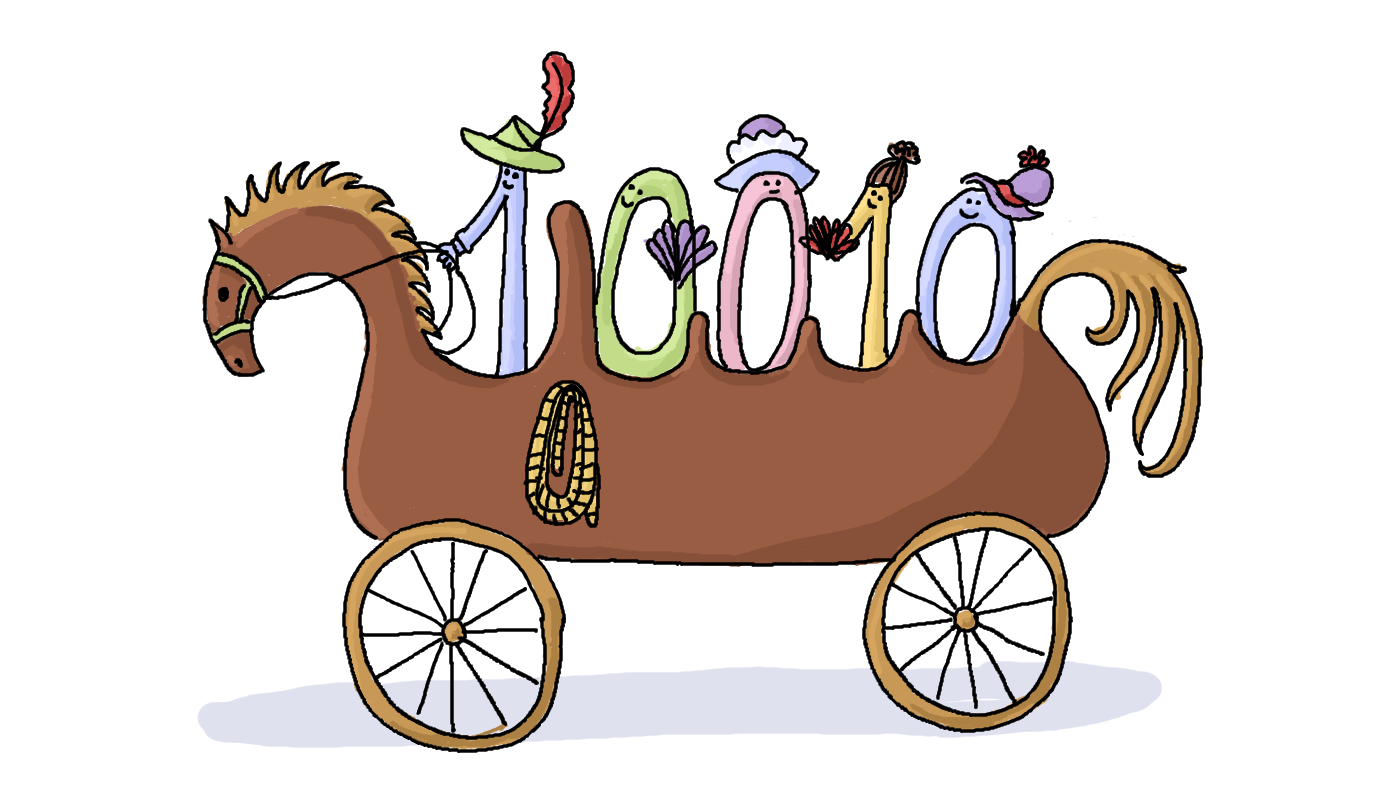
\includegraphics[width=\linewidth]{Pictures/Kutsche.png} 
\end{figure}

\tableofcontents

\section{Einführung}
Wie können Computer so viele unterschiedliche Dinge mit nur Nullen und Einser darstellen? Auf dem Bildschirm sehen wir Texte, Bilder, Videos, die wir noch dazu verändern können.

Vorletzte Woche haben wir gesehen, wie Computer ganze Zahlen speichern und manipulieren. Sie stellen die Zahlen in Basis 2 dar und speichern eine feste Anzahl Bits.

\begin{aufgabe}
Schreibe folgende Zahlen in der 32-Bit Zweierkomplement Darstellung:
\begin{enumerate}[(a)]
\item \(5\)
\item \(-1\)
\item \(25\)
\item \(-25\)
\end{enumerate}
\end{aufgabe}

Letzte Woche haben wir angefangen, uns mit der Darstellung der reellen Zahlen zu beschäftigen, mit den \textbf{Fliesskommazahlen}. Heute machen wir damit weiter.

Die Fliesskommazahlen, wie wir gesehen haben, sind im Grunde genommen nichts anderes, als die \textbf{Exponentialschreibweise}, die wir schon aus Chemie und Physik kennen: Die \textbf{Mantisse} wird mit der Basis hoch einem \textbf{Exponenten} multipliziert.

Zum Beispiel, die Avogadro-Konstante schreiben die Chemiker als \(6.02214076 \cdot 10^{23}\), anstatt alle 24 Stellen anzugeben. In dieser Schreibweise lassen sich Zahlen der unterschiedlichsten Grössenordnungen kompakt und übersichtlich darstellen:
\begin{itemize}
\item Masse von einem Proton: \(1.673 \cdot 10^{-27}\) Kilogramm
\item Grösse eines Coronavirus: \(1,4 \cdot 10^{-7}\) Meter
\item Lichtgeschwindigkeit: \(2.998 \cdot 10^{8}\) Meter pro Sekunde
\item Durchmesser von der Andromedagalaxie: \(1.32 \cdot 10^{21}\) Meter
\end{itemize}

Im Unterschied zu Menschen, arbeitet der Computer meistens in der Basis \(2\) statt \(10\) und \textbf{schränkt} die Anzahl der möglichen signifikanten Stellen und Exponenten \textbf{ein}.

Um diese Einschränkungen sichtbar und anfassbar zu machen, hatten wir das \textbf{''Kasten-Seil''-Modell} eingeführt.

\begin{figure}[H]
\centering
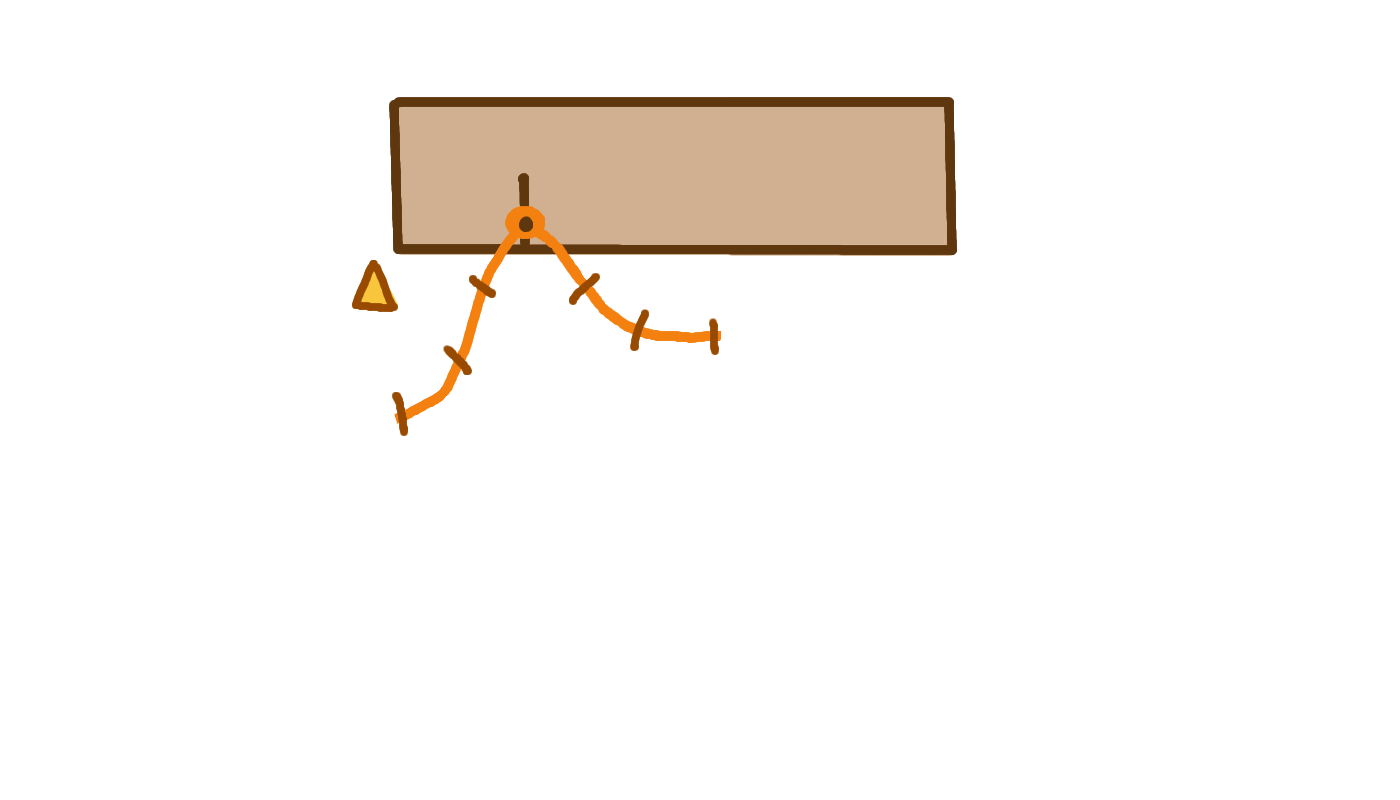
\includegraphics[width=0.75\linewidth]{Pictures/KastenOhneZahlen.png} 
\end{figure}

Das Modell besteht aus einem \textbf{Kasten}, in welchem wir eine fixe Anzahl Ziffern speichern können, und einem \textbf{Seil}, welches die Position vom Kasten bezüglich dem Komma speichert. Die Mitte vom Seil ist genau nach der ersten Stelle im Kasten befestigt und zwei Enden hängen lose: Das \textbf{negative Ende}  und das \textbf{positive Ende}. Auf dem Seil wird \textbf{markiert}, wo sich das Komma befindet.

Was machen wir, wenn wir folgende reelle Zahlen, binär in einer Fixkommadarstellung dargestellt, im ''Kasten-und-Seil''-Modell umschreiben wollen?

\begin{figure}[H]
\centering
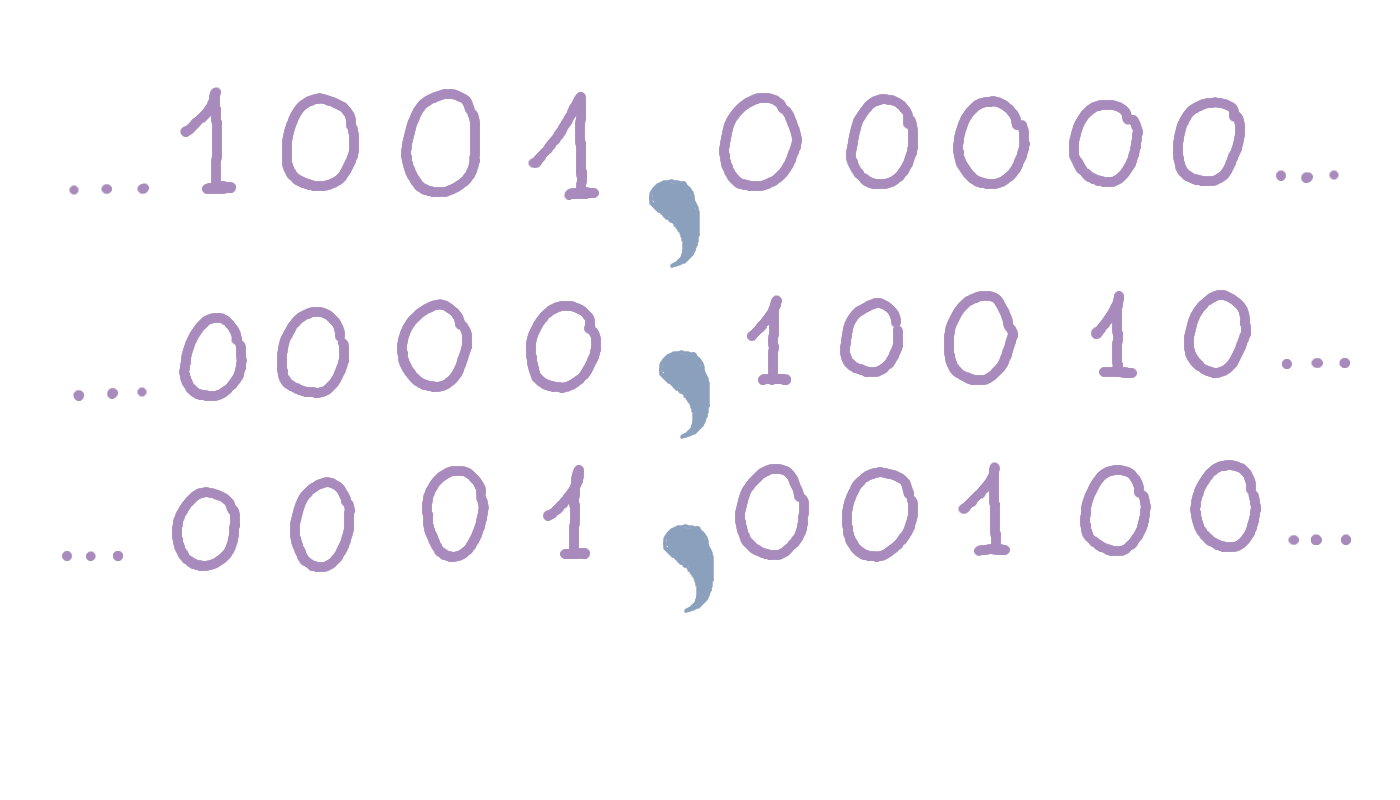
\includegraphics[width=0.65\linewidth]{Pictures/Zahlengerade.png} 
\end{figure}

Erstens, müssen wir bestimmen, wo wir den Kasten hinstellen, d.h. welche Ziffern gespeichert werden. Alle Ziffern, die sich ausserhalb vom Kasten befinden, gehen verloren. Es macht Sinn, die Ziffern mit dem grössten Wert zu nehmen, also mit der linkesten Eins anzufangen. Die Bits im Kasten sind die \textbf{Mantisse}.

\begin{figure}[H]
\centering
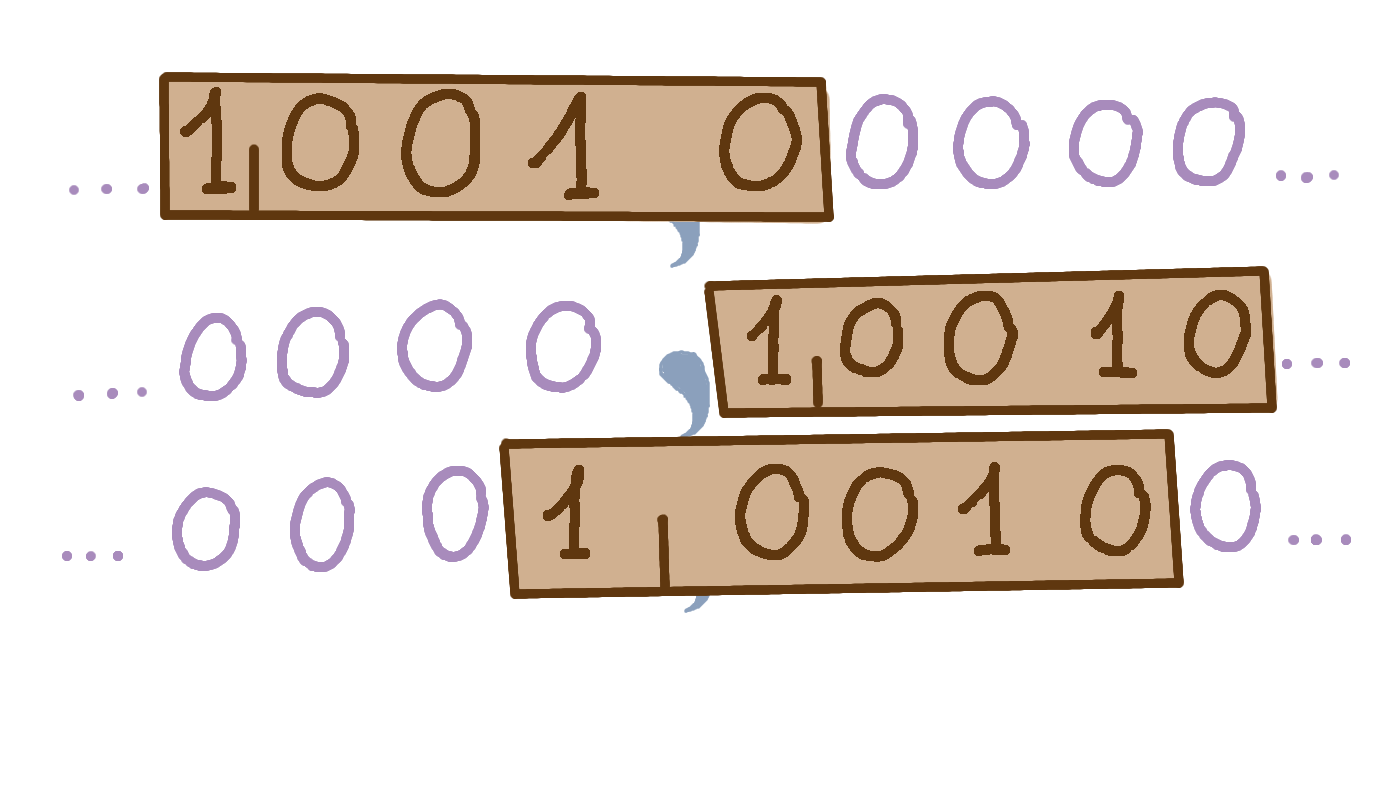
\includegraphics[width=0.65\linewidth]{Pictures/Kasten.png} 
\end{figure}

Nun haben wir 3 Kasten mit genau dem gleichen Inhalt: \texttt{10010}. Um die ursprünglichen Zahlen rekonstruieren zu können, müssen wir uns auch die Position des Kastens bezüglich dem Komma merken. Das machen wir im zweiten Schritt mit dem Seil. Die Mitte vom Seil wird gleich nach der linkesten Ziffer im Kasten befestigt, und die Position vom Komma wird am Seil markiert. Die Markierung auf dem Seil modelliert den \textbf{Exponenten}.

\begin{figure}[H]
\centering
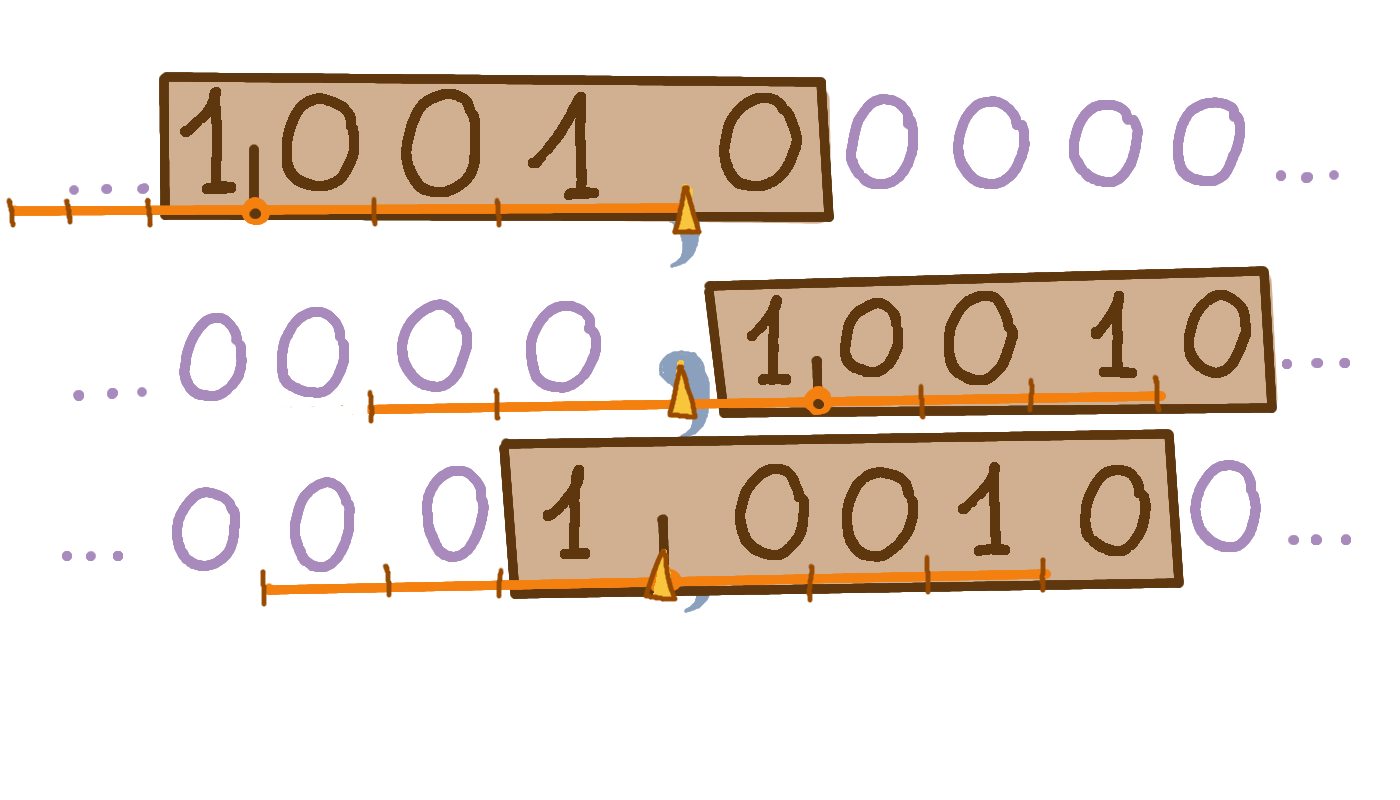
\includegraphics[width=0.65\linewidth]{Pictures/KastenMitSeil.png} 
\end{figure}

Jetzt haben wir alle Informationen gespeichert, die wir brauchen, um die ursprünglichen Zahlen wiederherzustellen. Damit diese Darstellung eindeutig ist, verlangen wir, dass das erste Bit der Mantisse eine Eins ist.

Folgende Elemente charakterisieren ein Fliesskommazahlensystem: Die Grösse vom Kasten, d.h. die \textbf{Mantissenlänge}, und die Länge vom Seil, d.h. der \textbf{Exponentenbereich}. Die Bits im Kasten und die Markierung am Seil stellen eine Zahl dar.

Der Computer hat intern keine Kasten und keine Seile. Er arbeitet mit Bitmuster. Jede Zahl hat eine fixe Anzahl Bits, typischerweise 32 (float) oder 64 (double), und diese Bits werden in \(3\) Bereiche aufgeteilt:
\begin{itemize}
\item Vorzeichen (grün auf dem Bild),
\item Exponent (Orange auf dem Bild),
\item Mantisse (braun auf dem Bild). 
\end{itemize}
Im Vorzeichenteil wird das \textbf{Vorzeichen} kodiert: \texttt{0} für positive Zahlen und \texttt{1} für negative.

Im Exponententeil wird die Markierung am Seil kodiert. Damit positive und negative Exponente in der fixen Anzahl Bits kodiert werden können, ein  \textbf{Biaswert} wird zum Exponenten addiert, so dass die \(0\) mit \texttt{1000...0} kodiert wird.

Im Mantissenteil werden die Bits aus dem Kasten gespeichert. Da das erste Bit immer eine Eins ist, wird es im Computer nicht gespeichert (implizites oder verstecktes Bit). Hier wird deshalb die führende Eins immer in Klammern angeführt.
\begin{figure}[H]
\centering
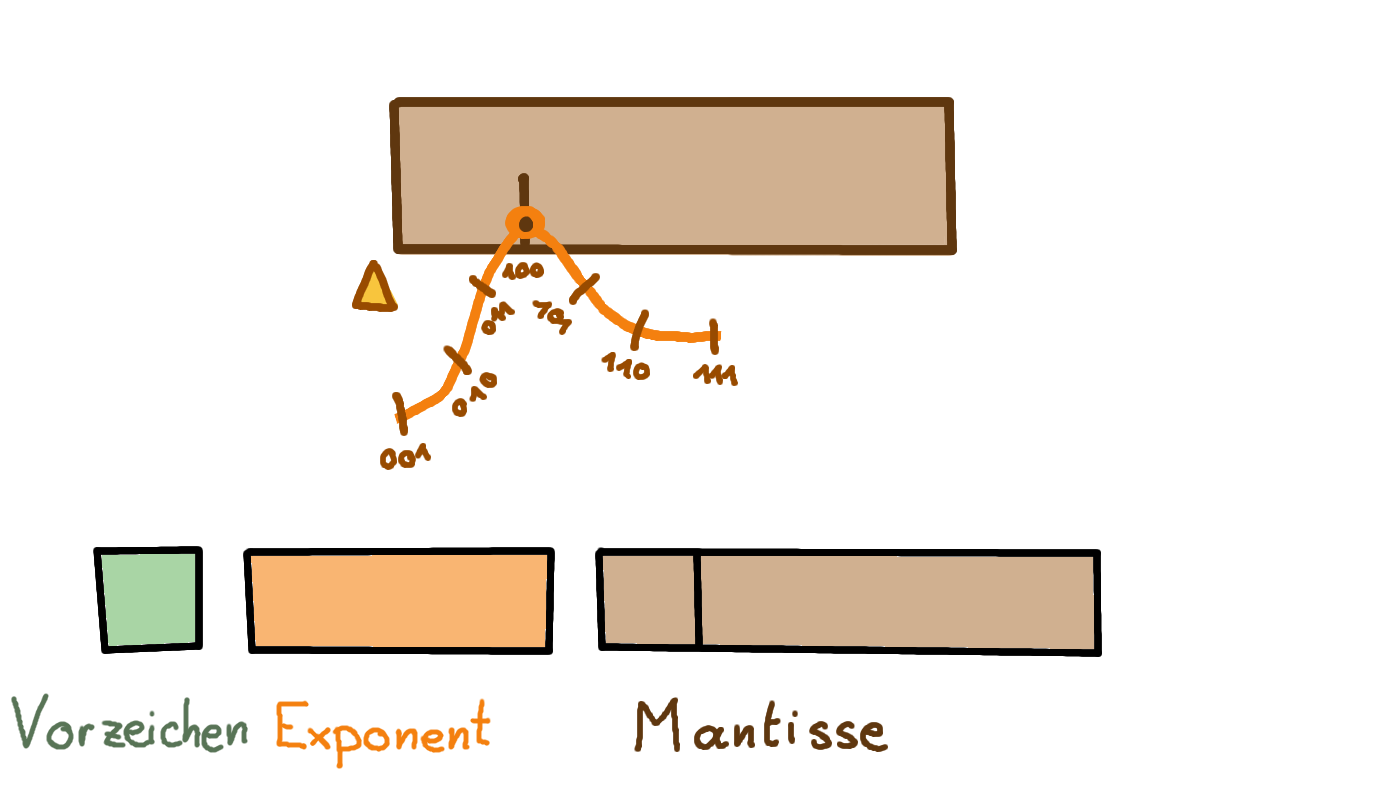
\includegraphics[width=0.75\linewidth]{Pictures/KastenMitSpeicher.png} 
\end{figure}

\begin{beispiel}
Wir werden zusammen die Zahl \(6.5\) im Fliesskommazahlensystem mit Mantissenlänge \(5\) und Exponenten von \(-3\) bis \(3\) darstellen.

Die reelle Zahl in Basis 2 in einer Fixkommadarstellung ist \(110.1\).

Der Kasten hat 5 Plätze. Alle signifikanten Stellen haben dort Platz. Dann verbinden wir das Seil mit dem Komma und setzen eine Markierung. Das lässt sich direkt ins Bitmuster übersetzen: Das Vorzeichen ist positiv, die Kodierung vom Exponenten lässt sich am Seil ablesen, die Mantisse speichert man direkt.
\begin{figure}[H]
\centering
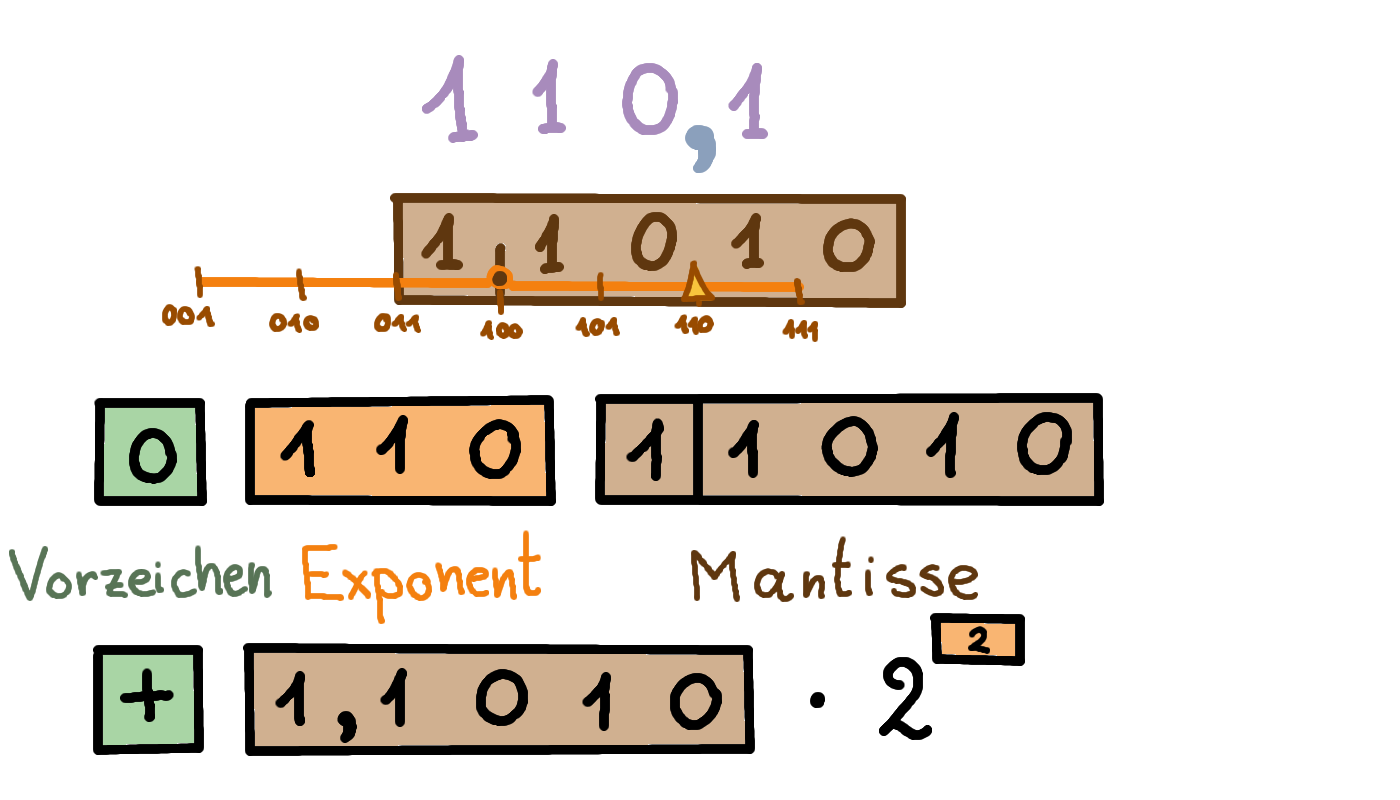
\includegraphics[width=0.75\linewidth]{Pictures/ZahlenDarstellen6-5.png} 
\end{figure}

\end{beispiel}

\begin{aufgabe}\label{einleitung-vom-kasten-nach-zahl}
Welche Zahl ist unten dargestellt? Vervollständige das Bitmuster und die Exponentialschreibweise und schreibe den Dezimalwert auf.

\begin{figure}[H]
\centering
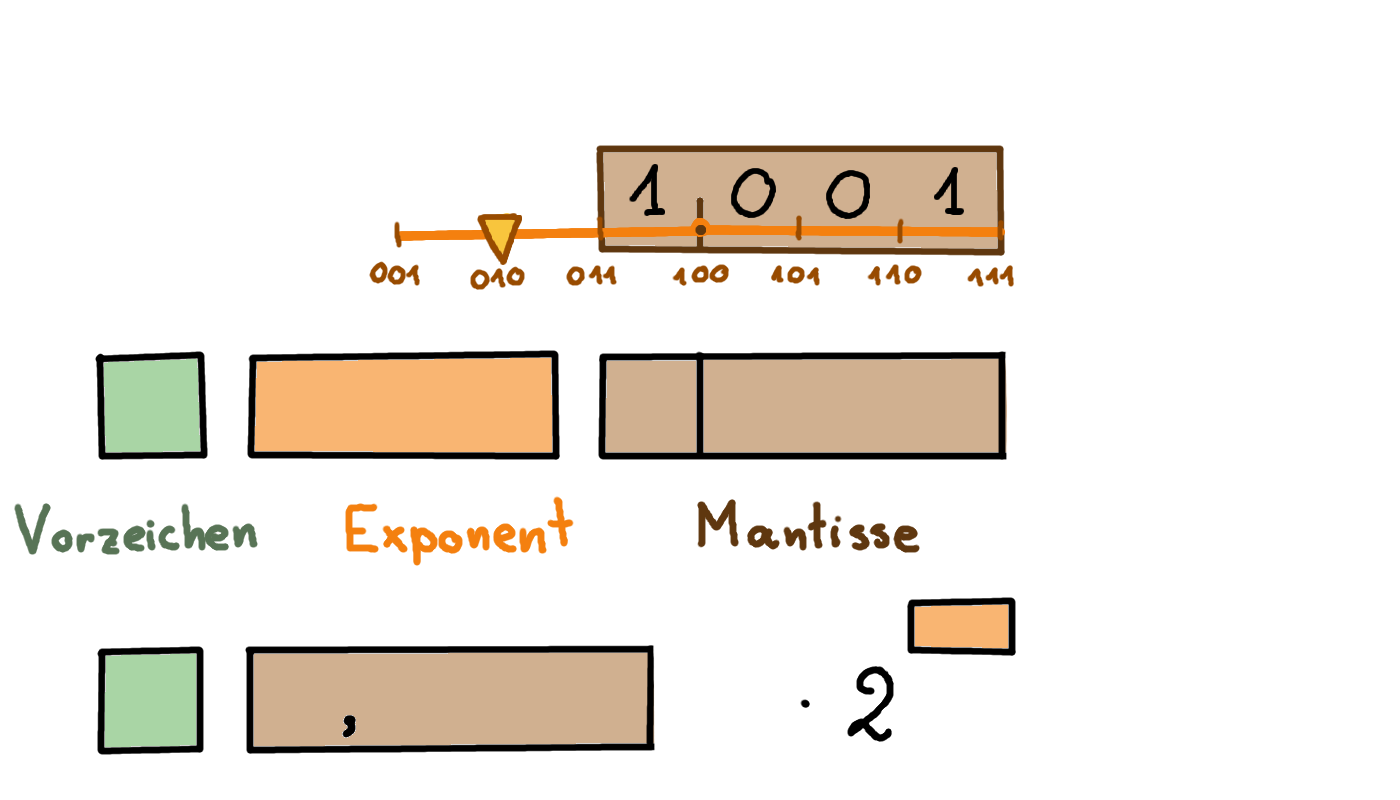
\includegraphics[width=0.8\linewidth]{Pictures/Einleitung_from_Kasten.png} 
\end{figure}
\end{aufgabe}

\begin{beispiel}
Nicht alle Zahlen lassen sich im Fliesskommazahlensystem genau darstellen. Manche müssen gerundet werden.
Zum Beispiel, die Zahl \(10.75\) sieht in Binär in einer Fixkommadarstellung so aus: \(1010.11\). Sie hat \(6\) signifikante Stellen, aber nur \(5\) haben in der Mantisse Platz. Die letzte Eins kann nicht gespeichert werden und geht verloren.
\begin{figure}[H]
\centering
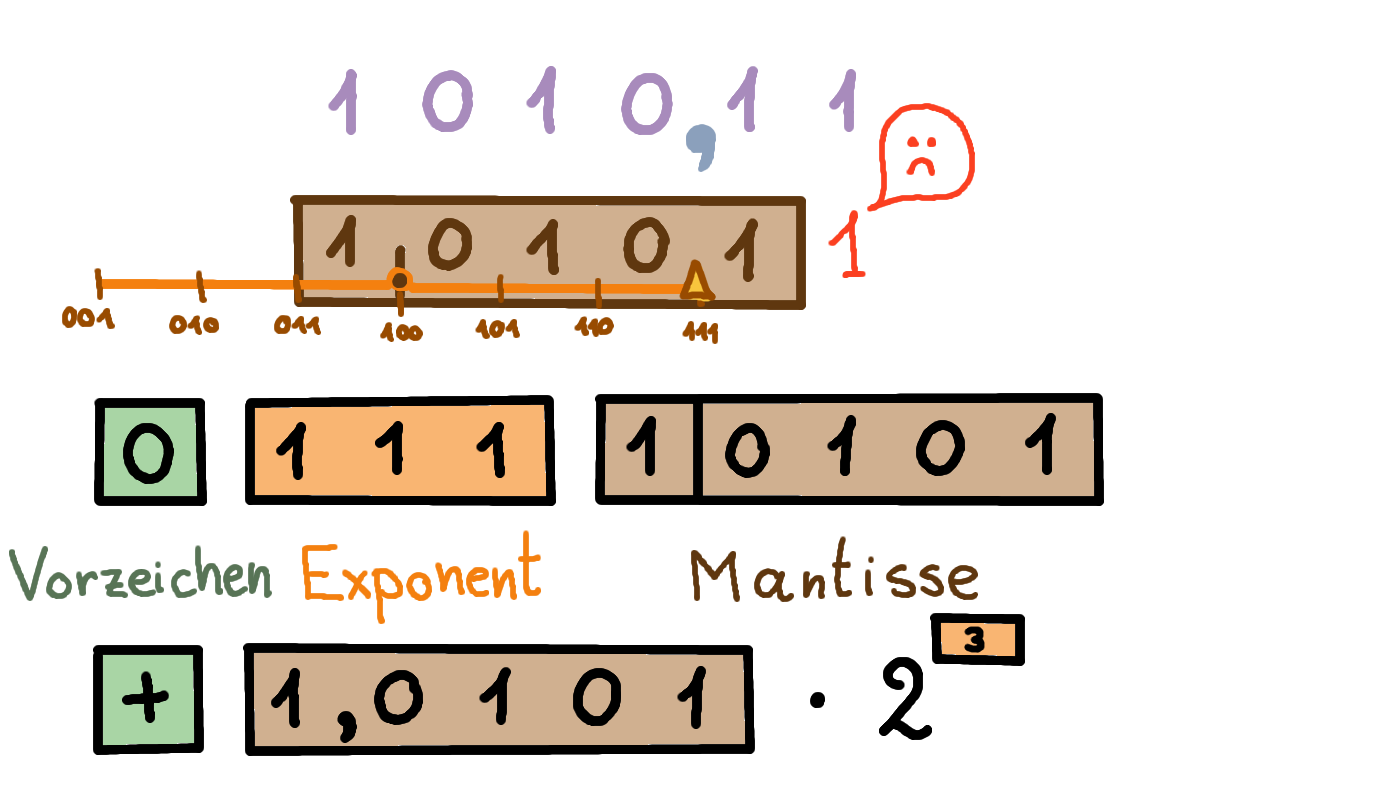
\includegraphics[width=0.75\linewidth]{Pictures/ZahlenDarstellen10-75.png} 
\end{figure}

\end{beispiel}
\newpage

\section{Fliesskommazahlen}
\subsection{Kleinste und grösste positive Zahlen}\label{sec:groesste-kleinste}

Es gibt unendlich viele reelle Zahlen. Wir können aber nur endlich viele davon in einem Fliesskommazahlensystem darstellen. Im Kasten, welcher uns die Mantisse veranschaulicht, finden nur endlich viele Bits Platz. Das Seil, welches den Kasten an den Komma bindet und welches uns den Exponenten veranschaulicht, hat ebenfalls eine endliche Länge.

Weil es endlich viele darstellbare Zahlen gibt, muss es eine kleinste und eine grösste Zahl geben. In diesem Abschnitt werden wir die kleinste und die grösste positive darstellbare Zahlen in Abhängigkeit vom Exponentenbereich und Mantissenlänge finden.


\begin{beispiel}
Wir konstruieren die grösste positive Zahl im Fliesskommazahlensystem mit Mantissenlänge \(5\) und Exponenten von \(-3\) bis \(3\).

In violett wird die reelle Zahl in Basis 2 aufgeschrieben, in der zweiten Zeile kommt die ''Kasten-und-Seil''-Darstellung aus der Einführung, in der dritten Zeile das Bitmuster und als letztes die Exponentialschreibweise. Darstellungsübergreifend ist die Mantisse in braun markiert, der Exponent in Orange und das Vorzeichen in grün.

Als erstes platzieren wir den Kasten. Damit die Zahl so gross wie möglich wird, muss der Kasten links vom Komma stehen, und zwar so weit entfernt wie möglich. Wir haben aber eine Einschränkung: Das Seil muss immer mit dem Komma verbunden bleiben.
\begin{figure}[H]
\centering
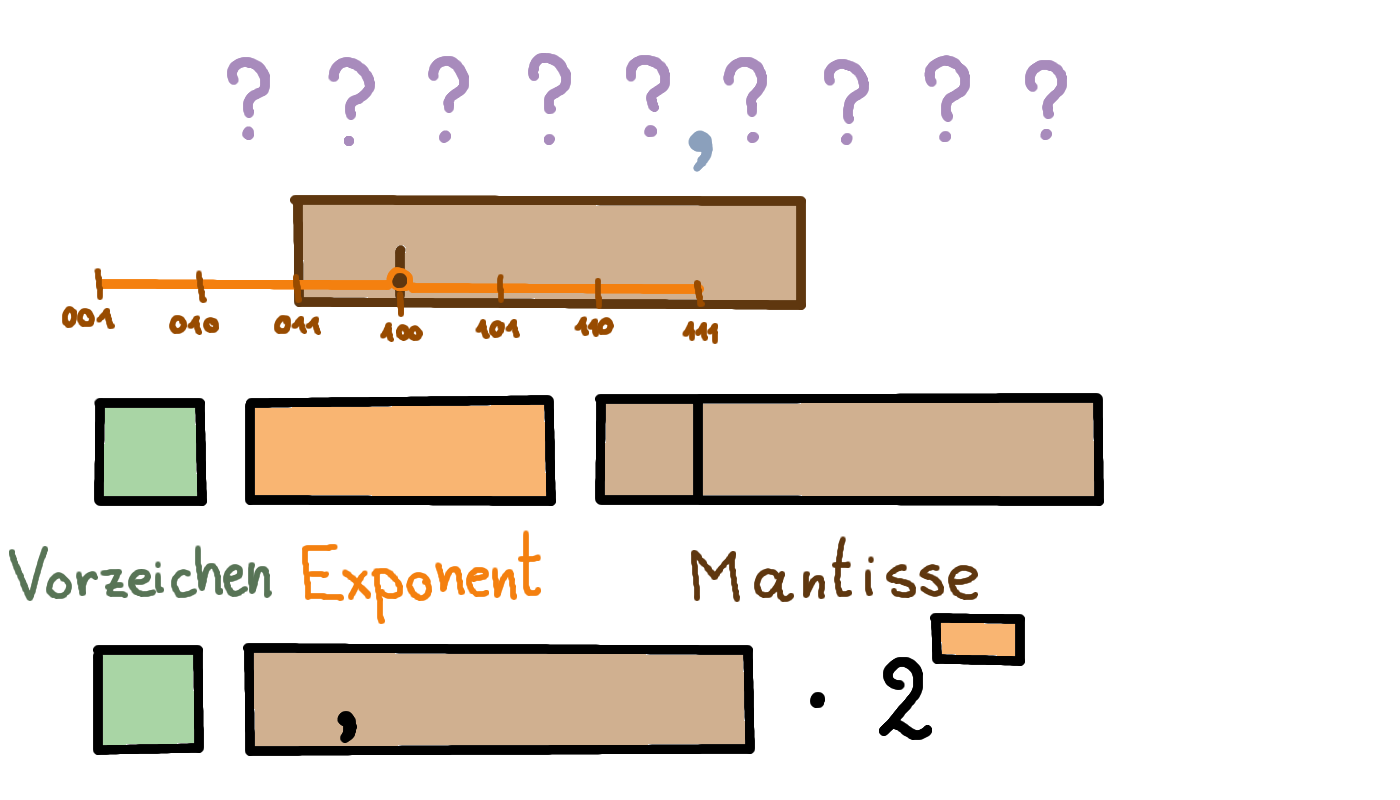
\includegraphics[width=0.85\linewidth]{Pictures/groessteZahl1.png}
\end{figure}
Der Exponent muss also möglichst gross sein.

Was ist mit der Mantisse? Sicher muss eine Eins an der ersten Stelle stehen.
\begin{figure}[H]
\centering
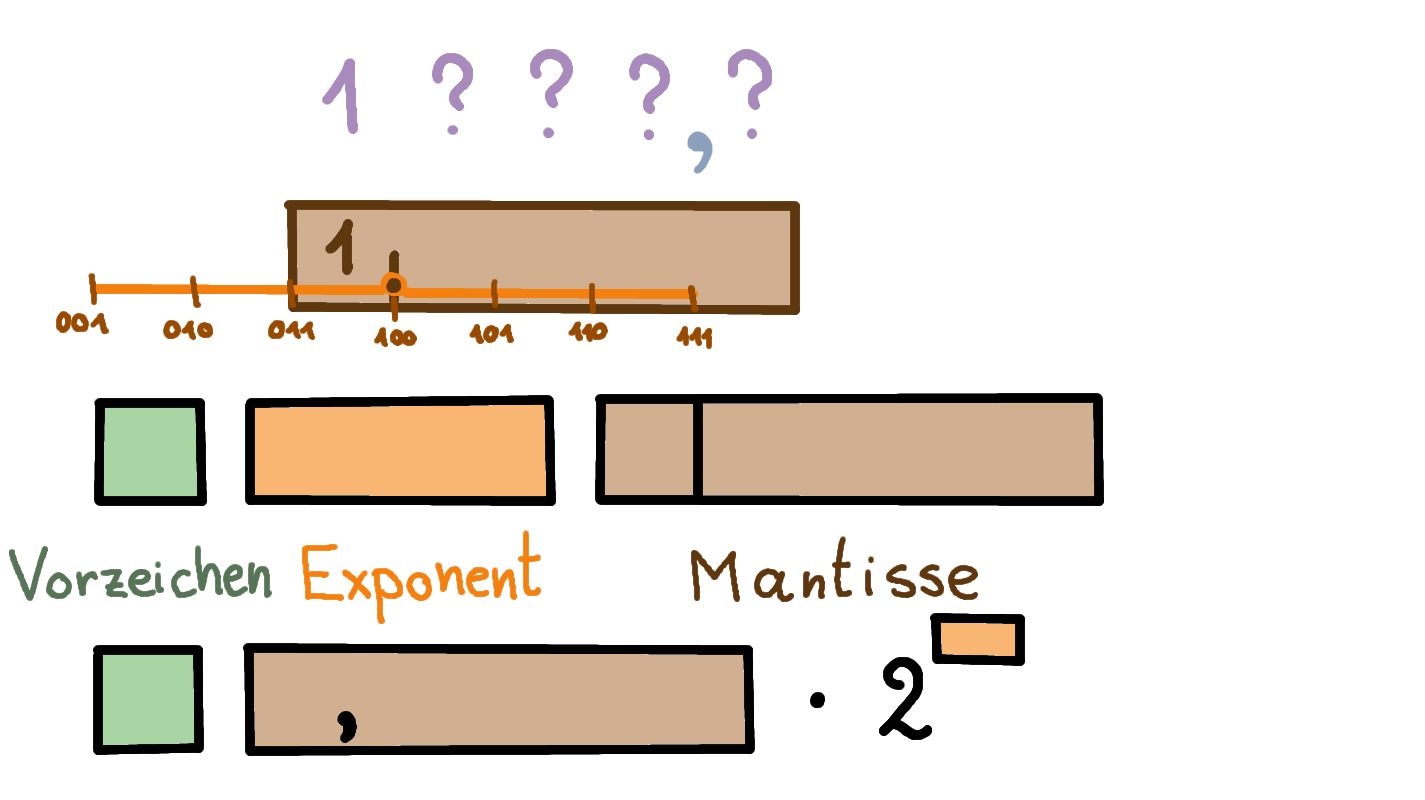
\includegraphics[width=0.85\linewidth]{Pictures/groessteZahl2.png}
\end{figure}

Damit die Mantisse möglichst gross wird, muss sie aus lauter Einser bestehen.
\begin{figure}[H]
\centering
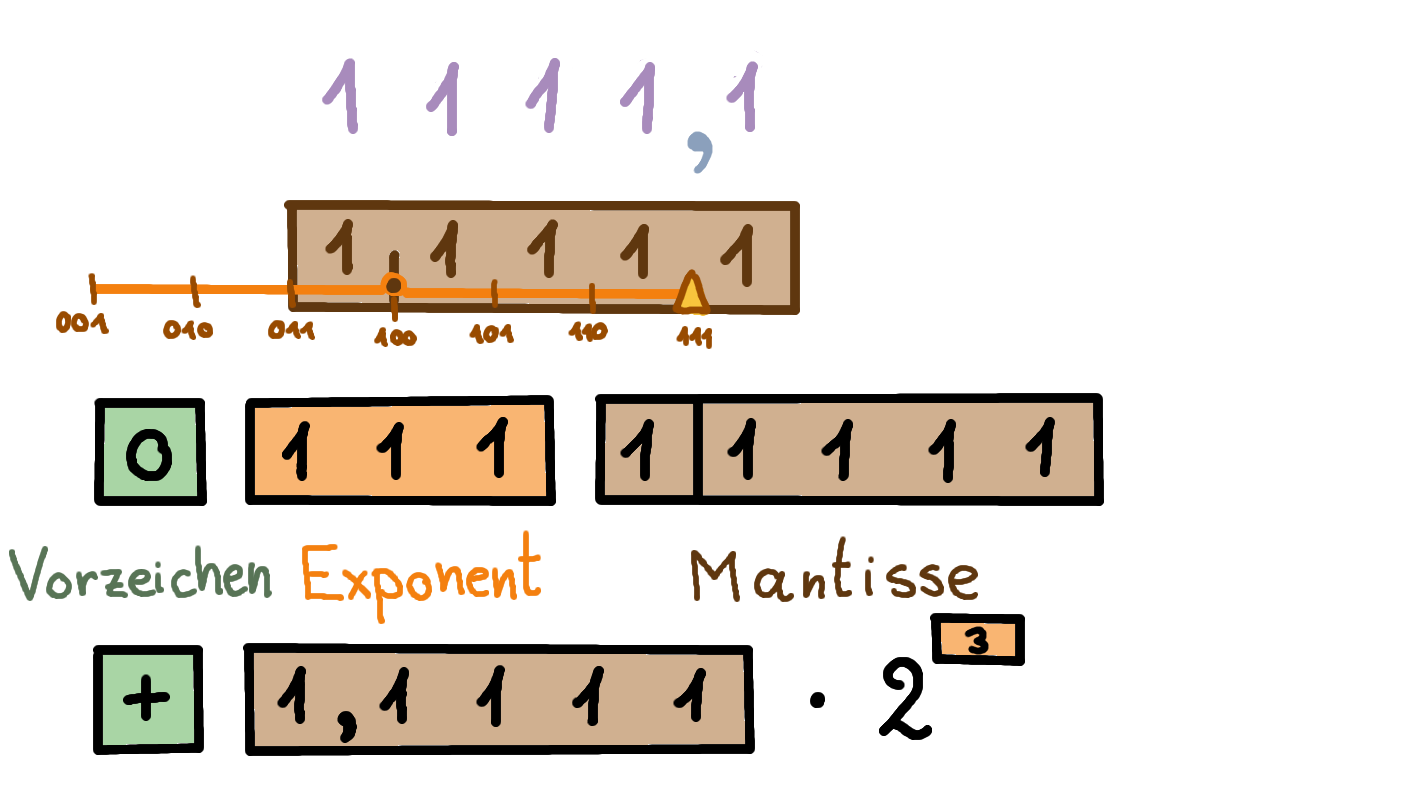
\includegraphics[width=0.85\linewidth]{Pictures/groessteZahl3.png}
\end{figure}

Die grösste darstellbare Zahl in diesem Fliesskommazahlensystem ist also \(15.5\).
\end{beispiel}

\begin{aufgabe}\label{kleinsteZahl-5-3}
Konstruiere die kleinste positive Zahl im Fliesskommazahlensystem mit Mantissenlänge \(5\) und Exponenten von \(-3\) bis \(3\). Schreibe die Zahl im ''Kasten-und-Seil''-Modell, als Bitmuster und in der binären Exponentialschreibweise auf und berechne ihren Dezimalwert.
\end{aufgabe}

Wir haben gesehen, dass die positive Zahlen, welche sich exakt in einem Fliesskommazahlensystem mit Mantissenlänge 5 und 3 Bits für den Exponenten darstellen lassen, zwischen \(1/8\) und \(15.5\) liegen müssen. Wie stark verändern sich diese Werte, wenn wir ein Bit weniger für die Mantisse zur Verfügung stellen?

\begin{aufgabe}\label{groesste-kleinste-4-3}
Betrachte das Fliesskommazahlensystem mit Mantissenlänge \(4\) und Exponenten von \(-3\) bis \(3\). Was erwartest du für die grösste positive darstellabare Zahl? Ist sie kleiner oder grösser als \(15.5\)? Wie stark unterscheidet sie sich davon?

Und was erwartest du für die kleinste positive darstellbare Zahl? Ist sie grösser oder kleiner als \(1/8\)? Wie stark unterscheidet sie sich davon?

Konstruiere die grösste und die kleinste positive darstellbare Zahlen in diesem System.  Schreibe die Zahlen im ''Kasten-und-Seil''-Modell, als Bitmuster und in der binären Exponentialschreibweise auf und berechne den Dezimalwert. 
\end{aufgabe}

In der vorherigen Aufgabe hast du gesehen, welchen Einfluss die Mantissenlänge auf die grösste und kleinste positive darstellbare Zahlen haben. Das Ergebnis könnte überraschend kommen. Da wir ein Bit weniger für die Mantisse und gleich viele Bits für den Exponenten genommen haben, ist unser Bitmuste um ein Bit kürzer geworden und somit können wir höchstens halb so viele Zahlen darstellen als vorher. Trotzdem haben sich die grösste und die kleinste positive darstellbare Zahlen kaum verändert.

Was passiert, wenn wir nun ein Bit weniger für den Exponenten nehmen?

\begin{aufgabe}\label{groesste-kleinste-5-2}
Betrachte das Fliesskommazahlensystem mit Mantissenlänge \(5\) und mit nur \(2\) Bits, um den Exponenten zu kodieren.
\begin{enumerate}[(a)]
\item Welche Exponenten können wir mit \(2\) Bits darstellen? Wie lang wird das Seil? Zeichne das ''Kasten-und-Seil''-Modell für dieses Fliesskommazahlensystem.
\item Was erwartest du für die grösste und die kleinste positive darstellbaren Zahlen? Wie stark unterscheiden sie sich von \(15.5\) und \(1/8\)?
\item Konstruiere die grösste und die kleinste positive darstellbare Zahlen in diesem System.  Schreibe die Zahlen im ''Kasten-und-Seil''-Modell, als Bitmuster und in der binären Exponentialschreibweise auf und berechne den Dezimalwert.
\end{enumerate}
\end{aufgabe}

In der vorherigen Aufgabe hast du gesehen, welchen Einfluss die Länge der Exponentenkodierung auf die grösste und kleinste positive darstellbare Zahlen hat. Wie auch im Fliesskommazahlensystem mit Mantissenlänge \(4\) und \(3\) Bits für den Exponenten, können wir im Fliesskommazahlensystem aus Aufgabe \ref{groesste-kleinste-5-2} höchstens halb so viele Zahlen darstellen wie im Fliesskommazahlensystem mit Mantissenlänge \(5\) und \(3\) Bits für die Exponentenkodierung. Der Bereich der darstellbaren Zahlen hat sich dieses Mal extrem verändert.

\begin{aufgabe}\label{groesste-kleinste-allgemein}
Wie sehen die kleinste und die grösste positive darstellbare Zahlen im allgemeinen Fliesskommazahlensystem aus? Nehme Mantissenlänge \(m\) und Exponent zwischen \(e_{min}\) und \(e_{max}\) an. Schreibe die kleinste und die grösste positive darstellbare Zahl in diesem Fliesskommazahlensystem als Bitmuster und in der binären Exponentialdarstellung auf.
\end{aufgabe}



\subsection{Darstellbare Zahlen}

Wir wissen, dass es eine kleinste und eine grösste positive Zahl gibt, welche sich exakt in einem Fliesskommazahlensystem darstellen lassen. Dass man nicht alle unendlich viele reelle Zahlen zwischen diesen zwei Schranken darstellen kann, können wir uns denken. Die Frage ist nun, welche Zahlen sich darstellen lassen und wie sich der Abstand zwischen darstellbaren Zahlen verhält.

Hier und in den folgenden Kapiteln, falls nicht speziell vermerkt, werden wir mit Mantissenlänge \(5\) und Exponentenbereich von \(-3\) bis \(3\) arbeiten.

\begin{beispiel}
Nehmen wir eine Zahl zwischen 1/8 und 15.5 (die kleinste und grösste positive darstellbare Zahlen in diesem Fliesskommazahlensystem), zum Beispiel \(10.25\). Lässt sich diese Zahl darstellen?

\begin{figure}[H]
\centering
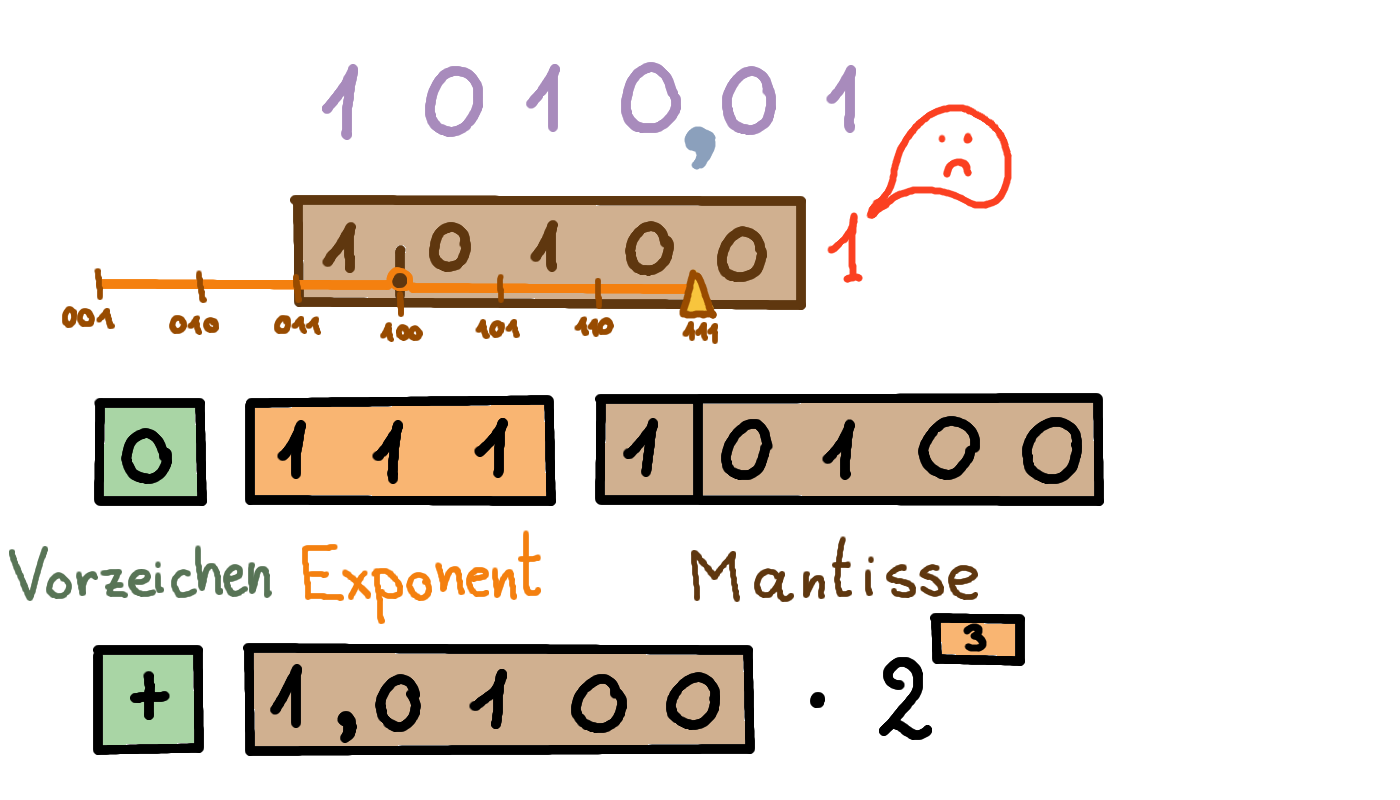
\includegraphics[width=0.75\linewidth]{Pictures/ZahlenDarstellen10-25.png}
\end{figure}

Diese Zahl lässt sich in gegebenem System nicht exakt darstellen. Für die letzte \(1\) gibt es in der Mantisse kein Platz. Deswegen wird \(10.25\) mit \(10.0\) \textbf{approximiert}.
\end{beispiel}

Wir haben gesehen, dass reelle Zahlen sich nur dann exakt darstellen lassen, wenn alle signifikante Stellen in der Mantisse Platz haben.

\begin{beispiel}
Betrachten wir die Zahl \(1\).

In einem Fliesskommazahlensystem lassen sich nur endlich viele Zahlen exakt darstellen. Einige von diesen darstellbaren Zahlen sind grösser als \(1\). Da es nur endlich davon gibt, muss es darunter eine kleinste geben. Diese Zahl bezeichnen wir hier als ''nächste'' oder ''nächstgrösste''. Die ''vorherige'' oder ''nächstkleinste'' darstellbare Zahl ist entsprechend die grösste unter den darstellbaren Zahlen, die kleiner als \(1\) sind.

Wie sieht die nächstgrösste Nachbarzahl von \(1\) aus?

Im ersten Schritt stellen wir die Zahl \(1\) im gegebenem Fliesskommazahlensystem dar.
\begin{figure}[H]
\centering
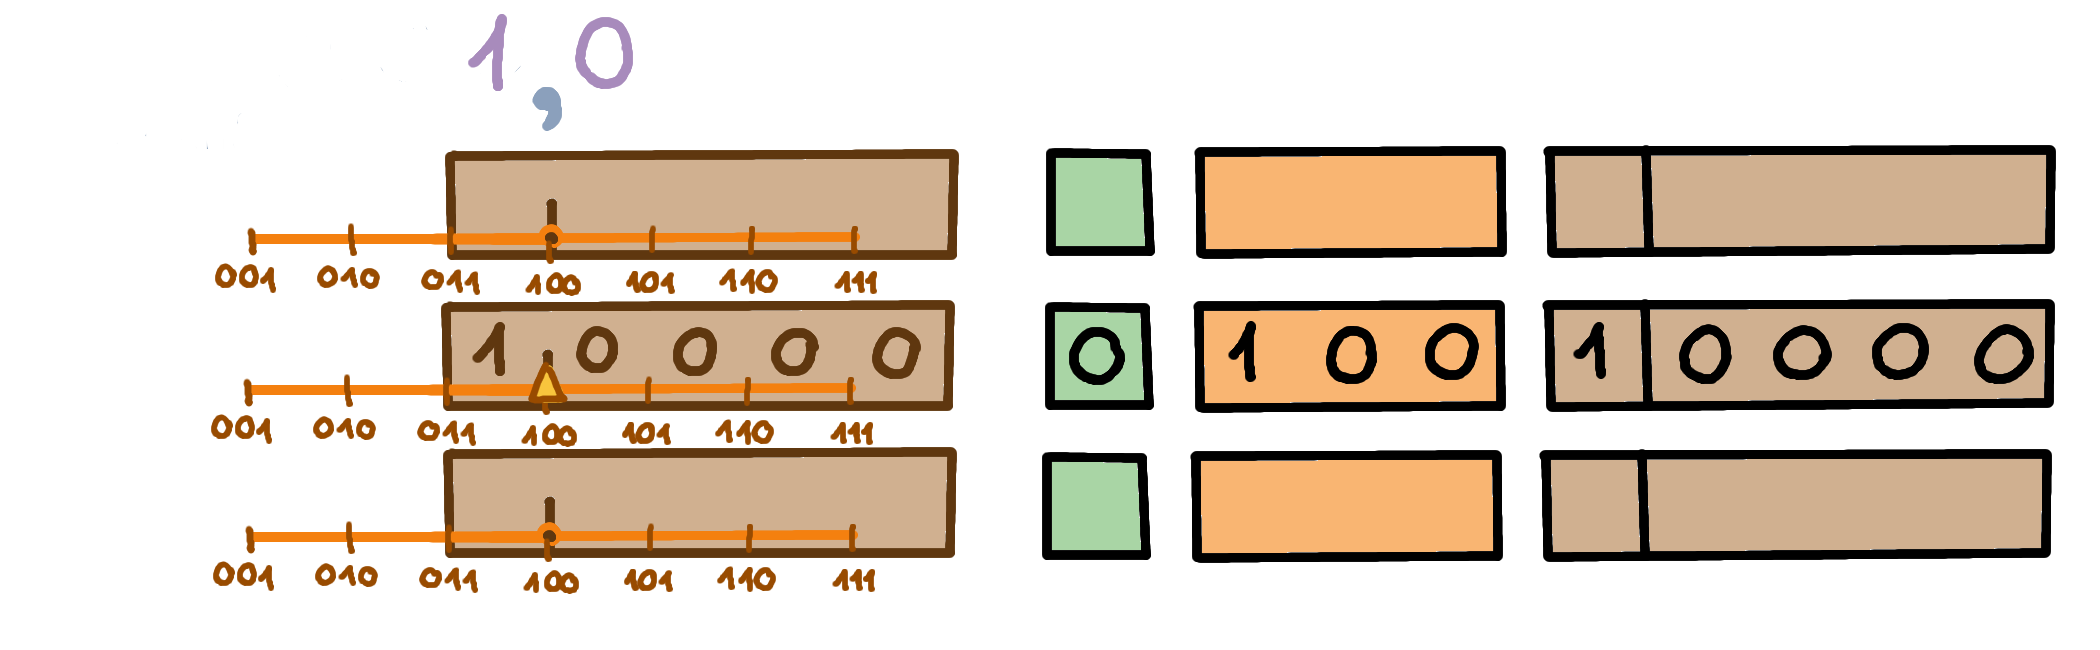
\includegraphics[width=\linewidth]{Pictures/Nachbarn1_1.png} 
\end{figure}

Wir suchen die Zahl, die minimal grösser als \(1\) ist.

Den Exponenten können wir in diesem Fall nicht verändern: Wenn wir den Kasten nach rechts bewegen, dann wird die Zahl kleiner; wenn wir den Kasten nach links bewegen, dann wird die Zahl wegen der obligatorischen führenden Eins zu gross.

Also müssen wir die Mantisse verändern. Da wir eine grössere Zahl suchen, müssen wir eine der Nullen zu einer Eins machen. Welche? Diejenige mit dem kleinsten Wert, d.h. die letzte Eins rechts.

\begin{figure}[H]
\centering
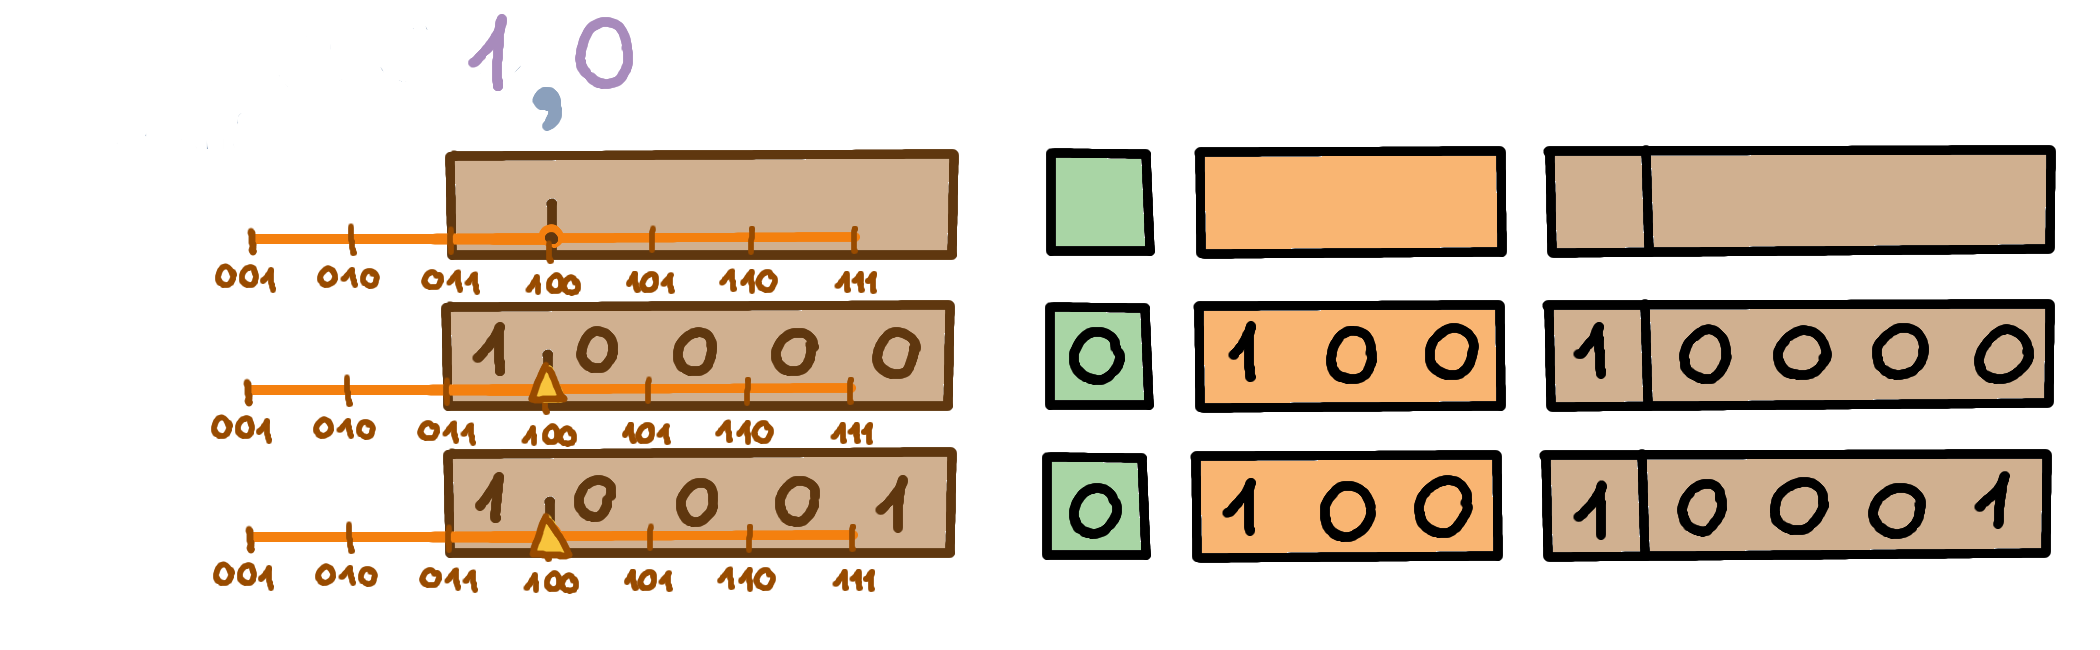
\includegraphics[width=\linewidth]{Pictures/Nachbarn1_N.png} 
\end{figure}
Die nächste darstellbare Zahl ist also \(1 + 1/16 = 17/16\).
\end{beispiel}

\begin{aufgabe}\label{nachbarn-vorherige}
Betrachte die Zahl \(1\). Finde die nächstkleinste darstellbare Zahl. Ist der Abstand zwischen der nächstkleinsten Zahl und \(1\) gleich dem Abstand zwischen \(1\) und der nächstgrössten Zahl?
\end{aufgabe}

\begin{aufgabe}\label{nachbarn}
Finde die nächste und die vorherige darstellbare Zahlen von folgenden Zahlen. Schreibe die Werte in der Dezimaldarstellung auf und stelle alle Zahlen als Bitmuster und in der Exponentialschreibweise dar. Bilde alle Zahlen, die in der Aufgabe und in deiner Lösung vorkommen, auf einem Zahlenstrahl ab. Was beobachtest du? Sind alle Nachbarn gleich entfernt?
\begin{enumerate}[(a)]
\item 2
\item 3
\item 4
\end{enumerate}
\end{aufgabe}

Im Abschnitt \ref{sec:groesste-kleinste} haben wir gesehen, dass die Länge der Exponentenkodierung deutlich mehr Einfluss auf dem darstellbaren Zahlenbereich hat als die Mantissenlänge. Ist das so auch für den Abstand zwischen Nachbarzahlen?

\begin{aufgabe}\label{nachbarn-laenge}
Betrachte die Zahl \(1\).

\begin{enumerate}[(a)]
\item Fülle die vorherige und die nächste darstellbare Zahlen im Fliesskommazahlensystem mit Mantissenlänge \(4\) und Exponent zwischen \(-3\) und \(3\) aus.
\begin{figure}[H]
\centering
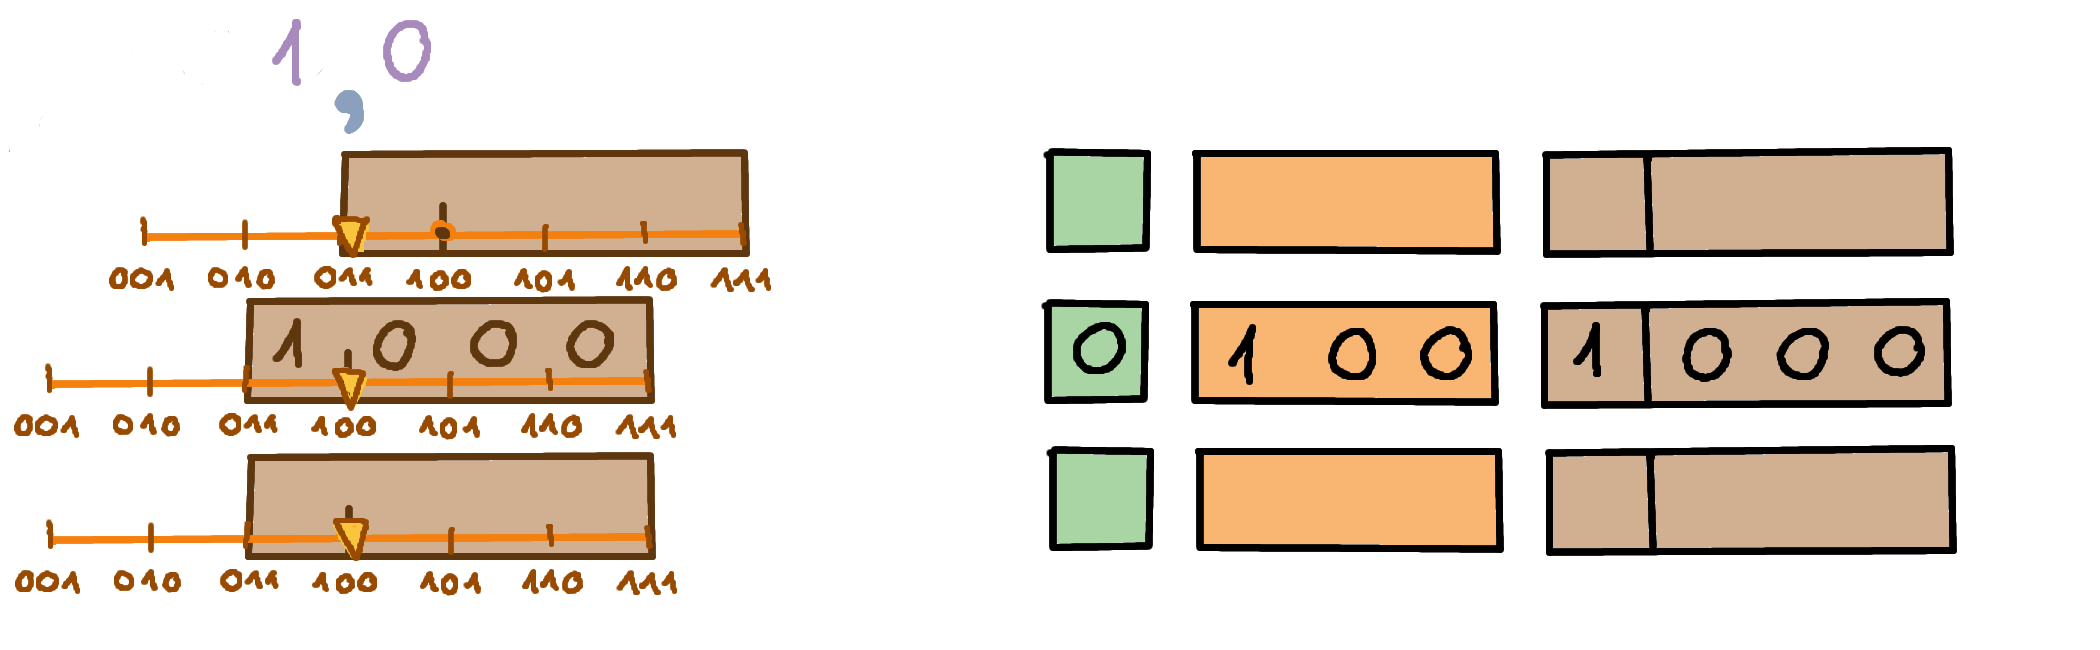
\includegraphics[width=\linewidth]{Pictures/Nachbarn1-4-3.png}
\end{figure}

\item Fülle die vorherige und die nächste darstellbare Zahlen im Fliesskommazahlensystem mit Mantissenlänge \(5\) und Exponent zwischen \(-1\) und \(1\) aus.
\begin{figure}[H]
\centering
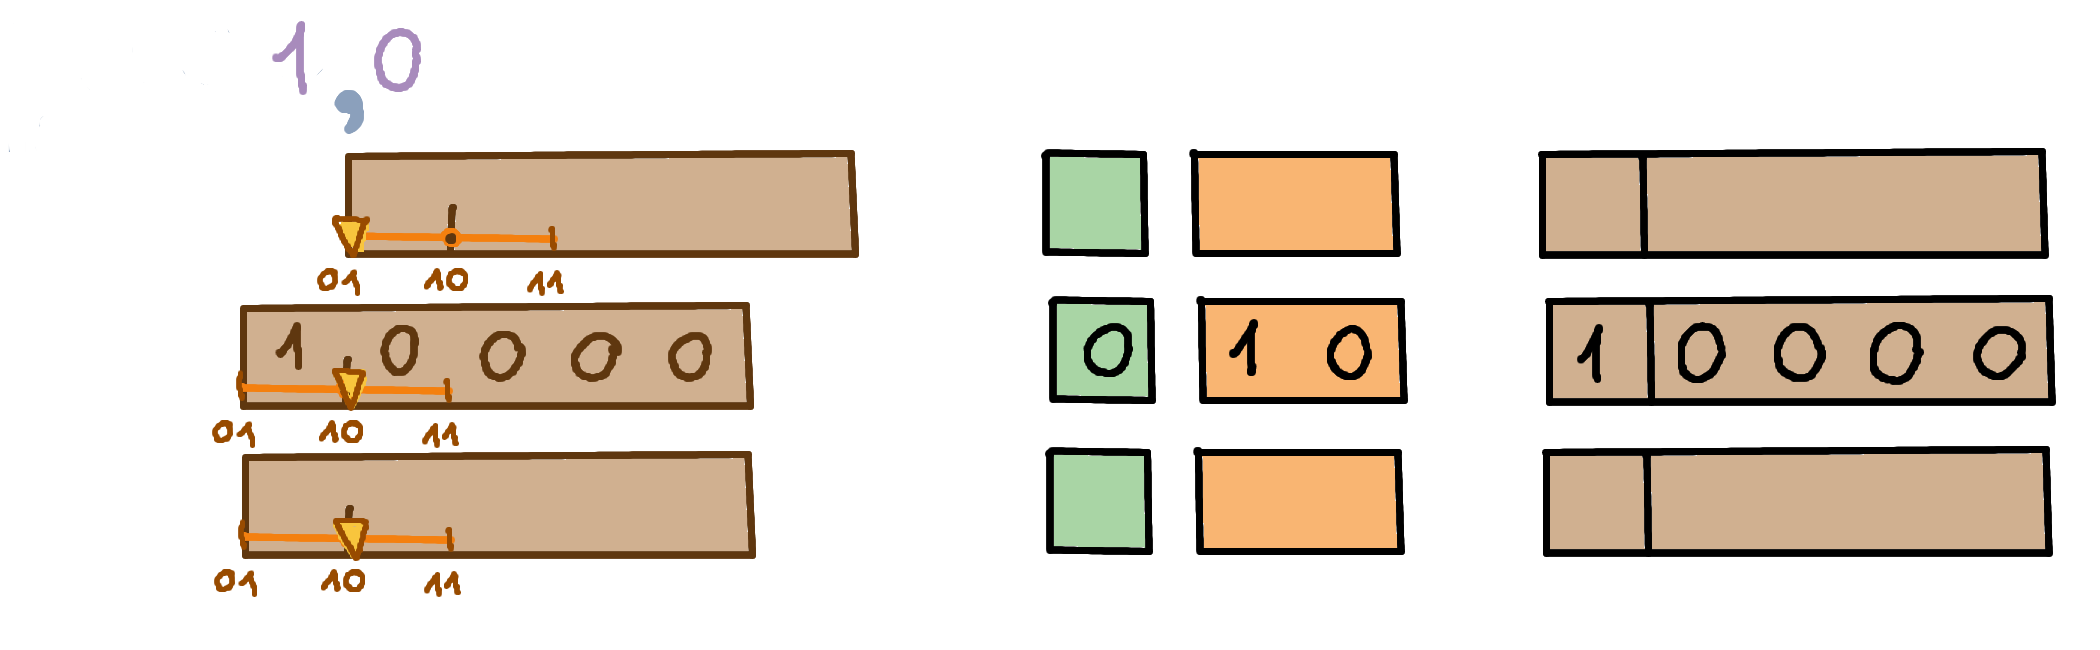
\includegraphics[width=\linewidth]{Pictures/Nachbarn1-5-2.png}
\end{figure}

\item Bei welchem Fliesskommazahlensystem ist der Abstand zwischen benachbarten Zahlen änhlich zu dem im Fliesskommazahlensystem mit Mantissenlänge \(5\) und Exponent zwischen \(-3\) und \(3\)?
\end{enumerate}

\end{aufgabe}

\subsubsection*{\textcolor{blue-violet}{Teste dich selber}}

\begin{aufgabe}\label{fliesskommazahlen_kontrollfragen}
Beantworte folgende Fragen:
\begin{enumerate}[(a)]
\item Kann man im Fliesskommazahlensystem alle reelle Zahlen darstellen? Wieso?
\item Gibt es eine grösste Zahl im Fliesskommazahlensystem? Falls nein, warum? Falls ja, wie findet man sie?
\item Gibt es eine kleinste Zahl im Fliesskommazahlensystem? Falls nein, warum? Falls ja, wie findet man sie?
\item Was beeinflusst stärker den Bereich der positiven darstellbaren Zahlen in einem Fliesskommasystem? Die Mantissenlänge oder die Länge der Exponentenkodierung?
\item Gib eine Zahl zwischen \(1/2\) und \(3.5\) an, die im Fliesskommazahlensystem mit Mantissenlänge \(3\) und Exponenten von \(-1\) bis \(1\) nicht darstellbar ist.
\item Sind alle Zahlen im Fliesskommazahlensystem gleichverteilt? Falls nicht, welche Zahlen stehen dichter beieinander, die kleineren oder die grösseren?
\item Was beeinflusst stärker den Abstand zwischen den positiven darstellbaren Zahlen in einem Fliesskommazahlensystem? Die Mantissenlänge oder die Länge der Exponentenkodierung?
\end{enumerate}
\end{aufgabe}

\newpage

\section{Addition}
Im vorherigen Kapitel haben wir gesehen, welche Zahlen in einem Fliesskommazahlensystem dargestellt werden können, das heisst welche Zahlen  exakt in einem Computer gespeichert werden können. Computer werden aber nicht nur zum Speichern von Zahlen verwendet, sondern auch für Berechnungen.  Auch bei Berechnungen verhalten sich Fliesskommazahlen nicht ganz wie reelle Zahlen. In diesem Kapitel werden wir dies am Beispiel der Addition erfahren. 

\begin{beispiel}
Wir möchten \(1/4 + 1/8\) ausrechnen. Der erste Schritt ist beide Zahlen aufzuschreiben. Wie in den vorherigen Kapiteln, sind in violett die reelle Zahlen in Basis 2 aufgeschrieben und braune ''Kasten'' mit orangenem ''Seil'' verwendet, um Mantisse und Exponent zu veranschaulichen. Rechts wird das Bitmuster in der gewöhnlichen Form angegeben.
\begin{figure}[H]
\centering
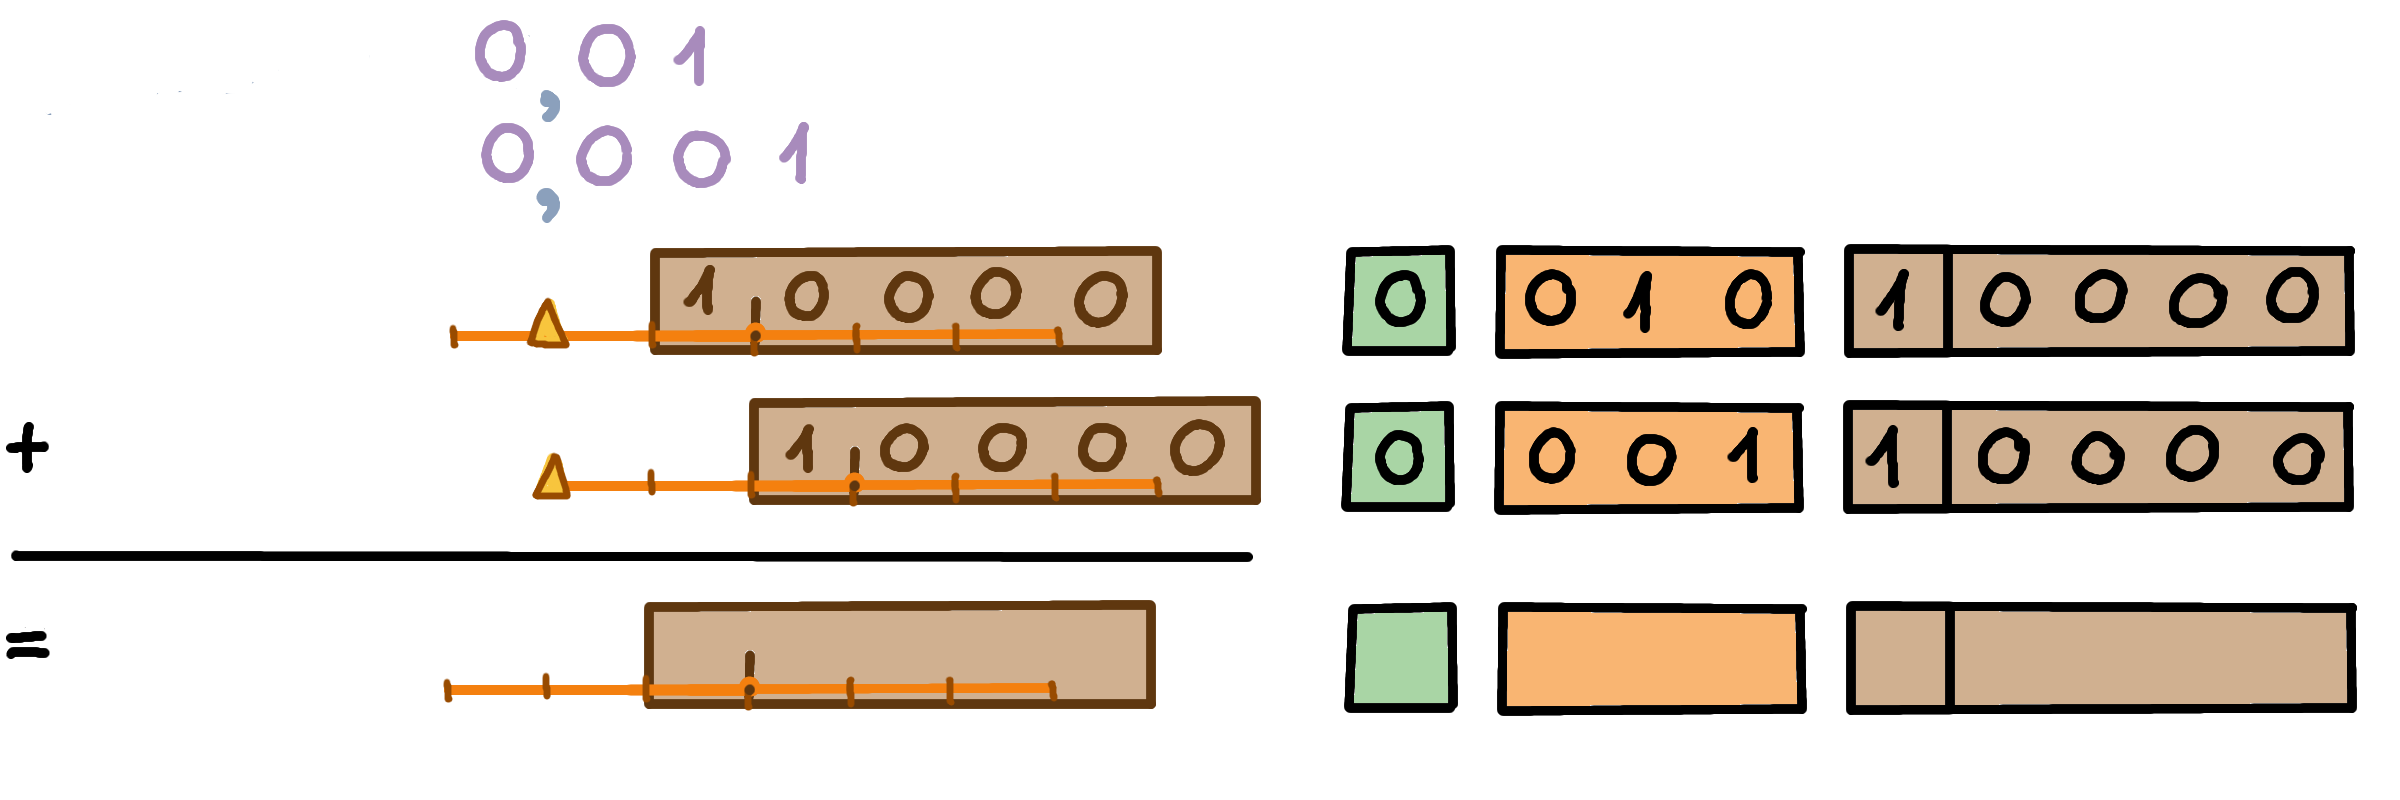
\includegraphics[width=\linewidth]{Pictures/Addition1-4and1-8_1.png}
\end{figure}

Damit wir die Bits der Mantisse stellenweise addieren können, wie wir das von den ganzen Zahlen kennen, müssen wir die zwei ''Kasten'' so verschieben, dass sie sich untereinander befinden. Da alles, was ausserhalb vom ''Kasten'' landet, verloren geht, werden wir den Kasten von der kleineren Zahl unter den Kasten von der grösseren Zahl schieben. So werden wir die Stellen mit dem niedrigsten Wert verlieren. In diesem Fall verlieren wir eine Null, der Wert der Zahl verändert sich also nicht.

Beachte, dass wenn der Kasten verschoben wird, verschiebt sich auch die Markierung bezüglich des ''Seils'', das heisst der Exponent verändert sich. Die Markierung am ''Seil'' bleibt immer unter dem Komma.
\begin{figure}[H]
\centering
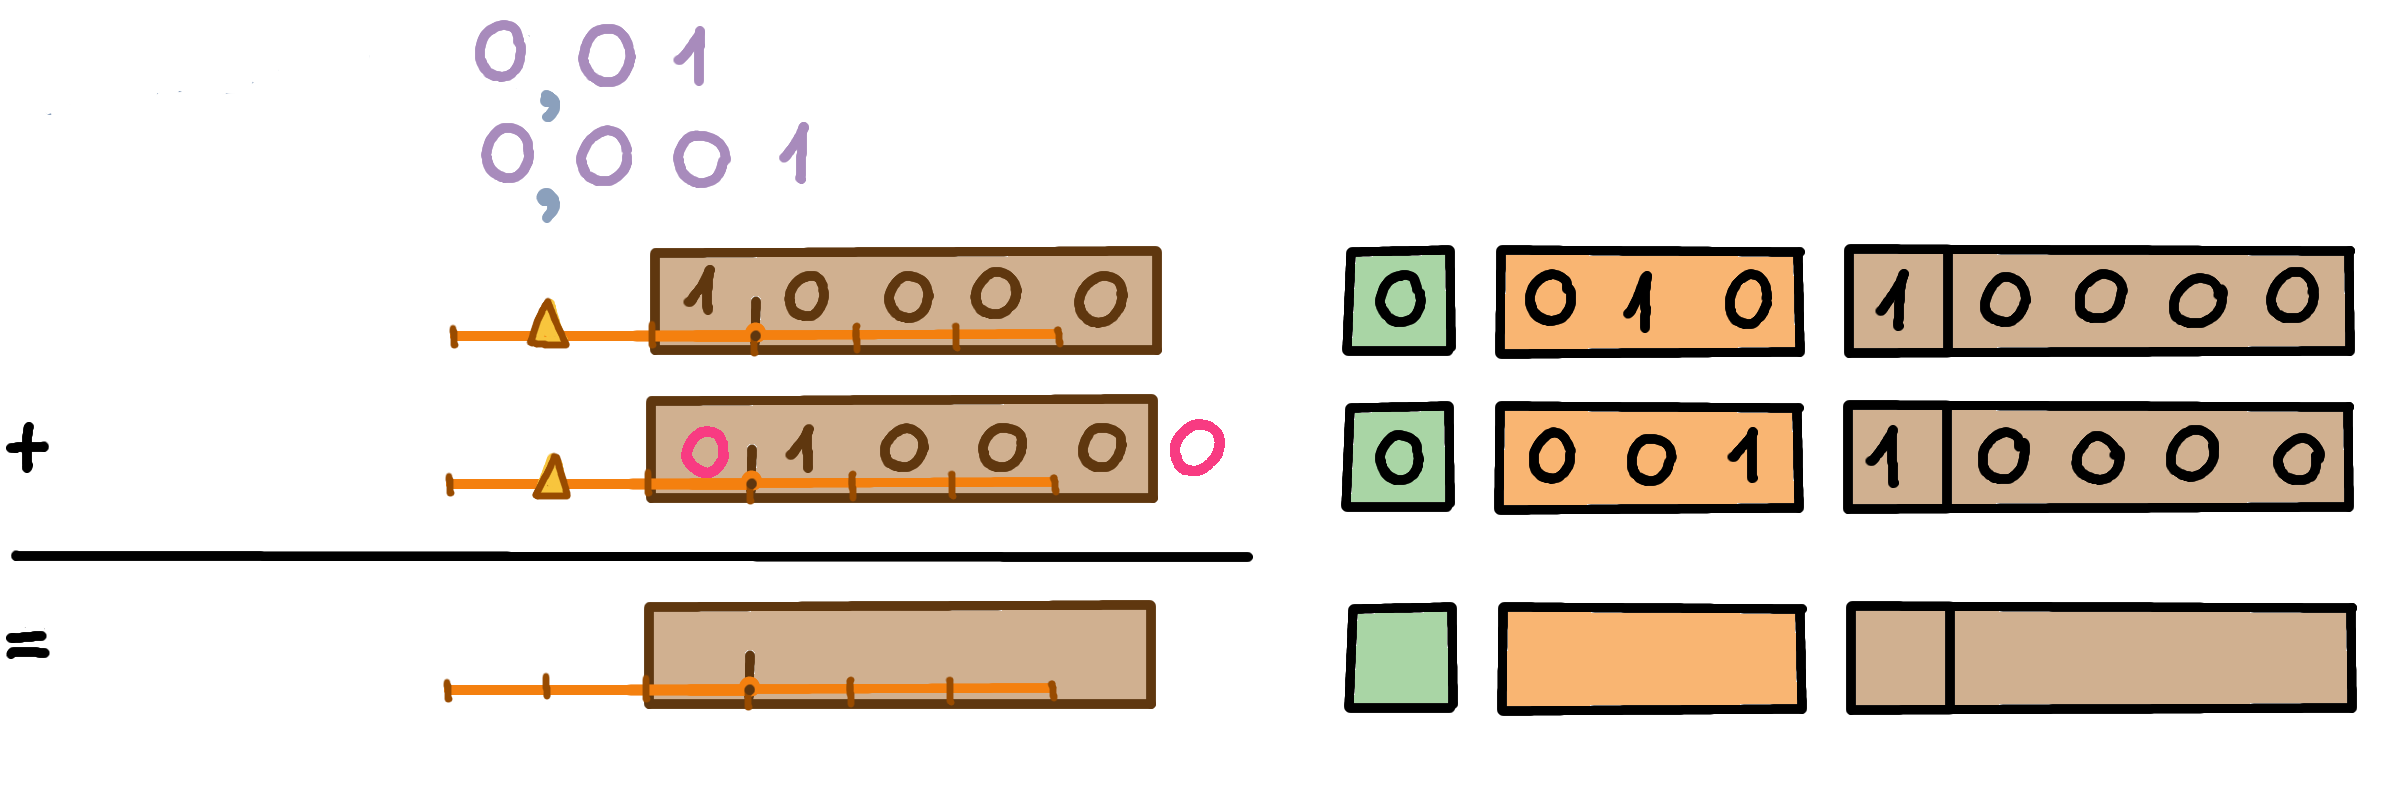
\includegraphics[width=\linewidth]{Pictures/Addition1-4and1-8_2.png}
\end{figure}

Wenn die Kasten untereinander sind, können wir die Bits in den Kasten wie gewöhnlich addieren, wie bei den Integers.
\begin{figure}[H]
\centering
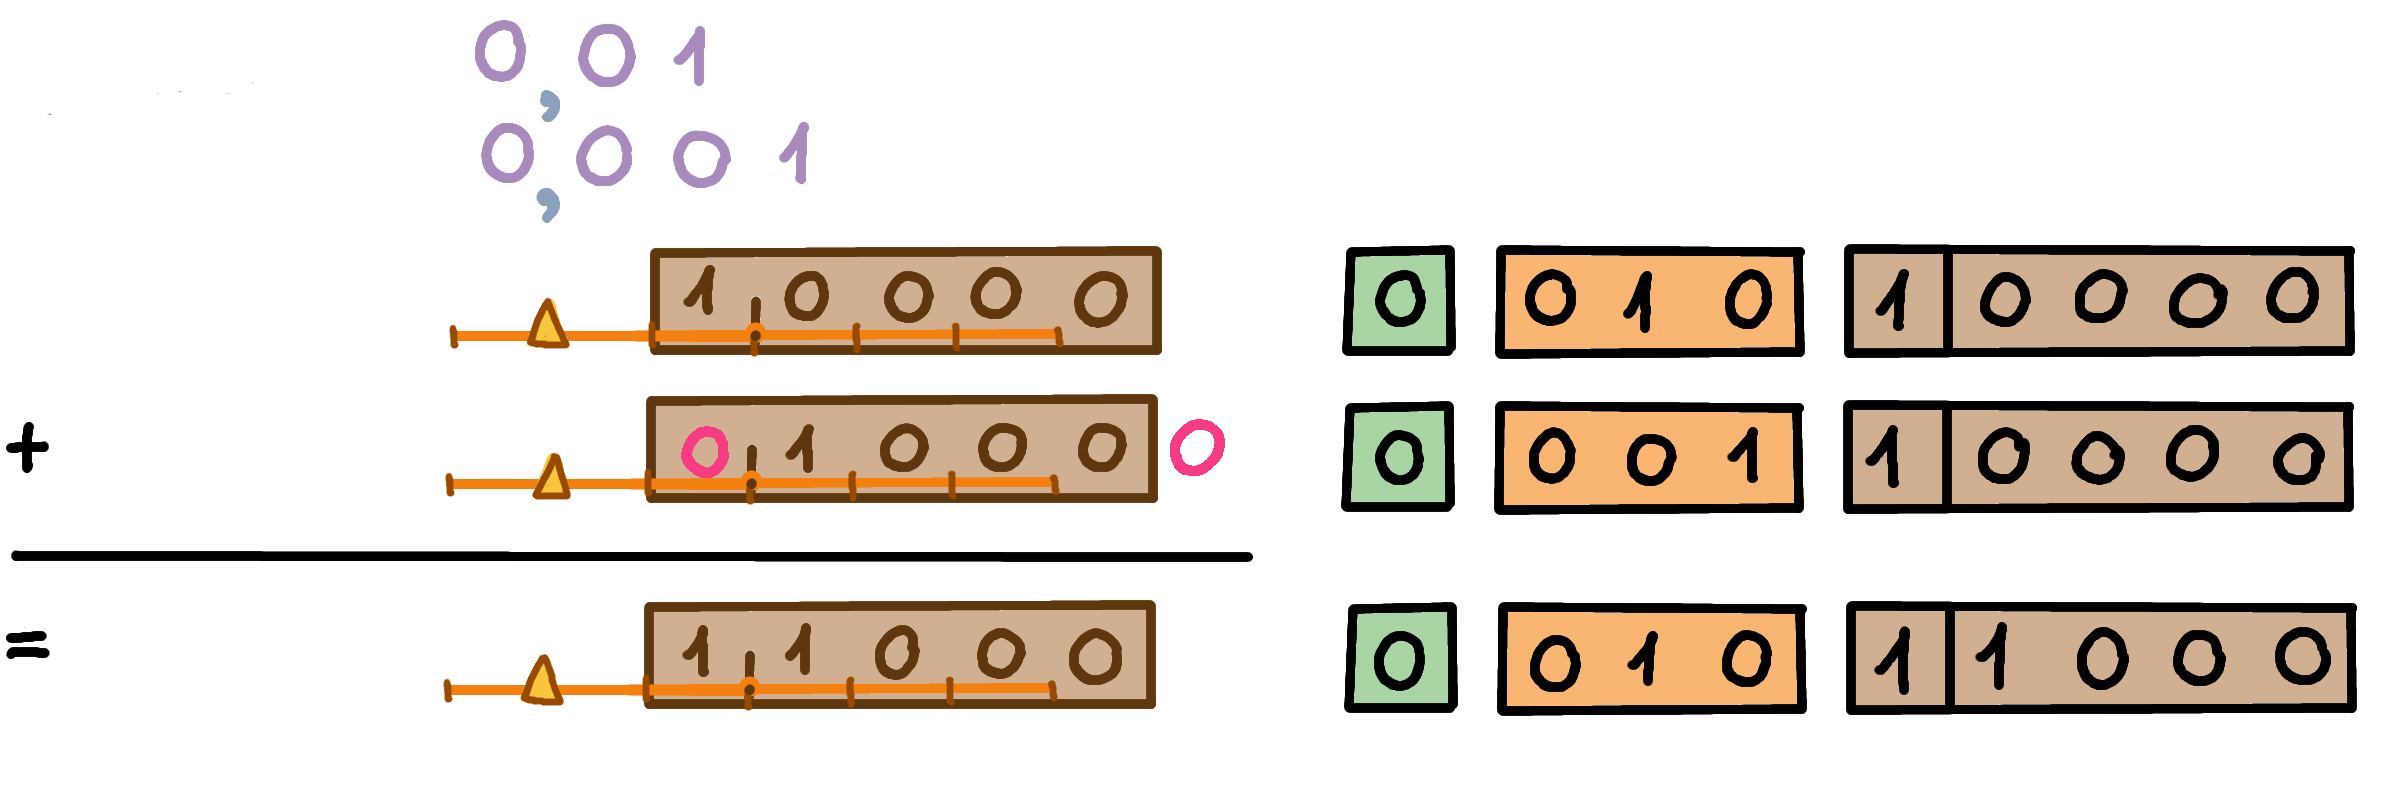
\includegraphics[width=\linewidth]{Pictures/Addition1-4and1-8_3.png}
\end{figure}
Wir haben ausgerechnet, dass \(1/4 + 1/8 = 3/8\), in der Exponentialschreibweise \(1.1000 \cdot 2^{-2}\).
\end{beispiel}

\begin{beispiel}
Wir möchten \(2+3\) ausrechnen. Im ersten Schritt schreiben wir beide Zahlen auf.
\begin{figure}[H]
\centering
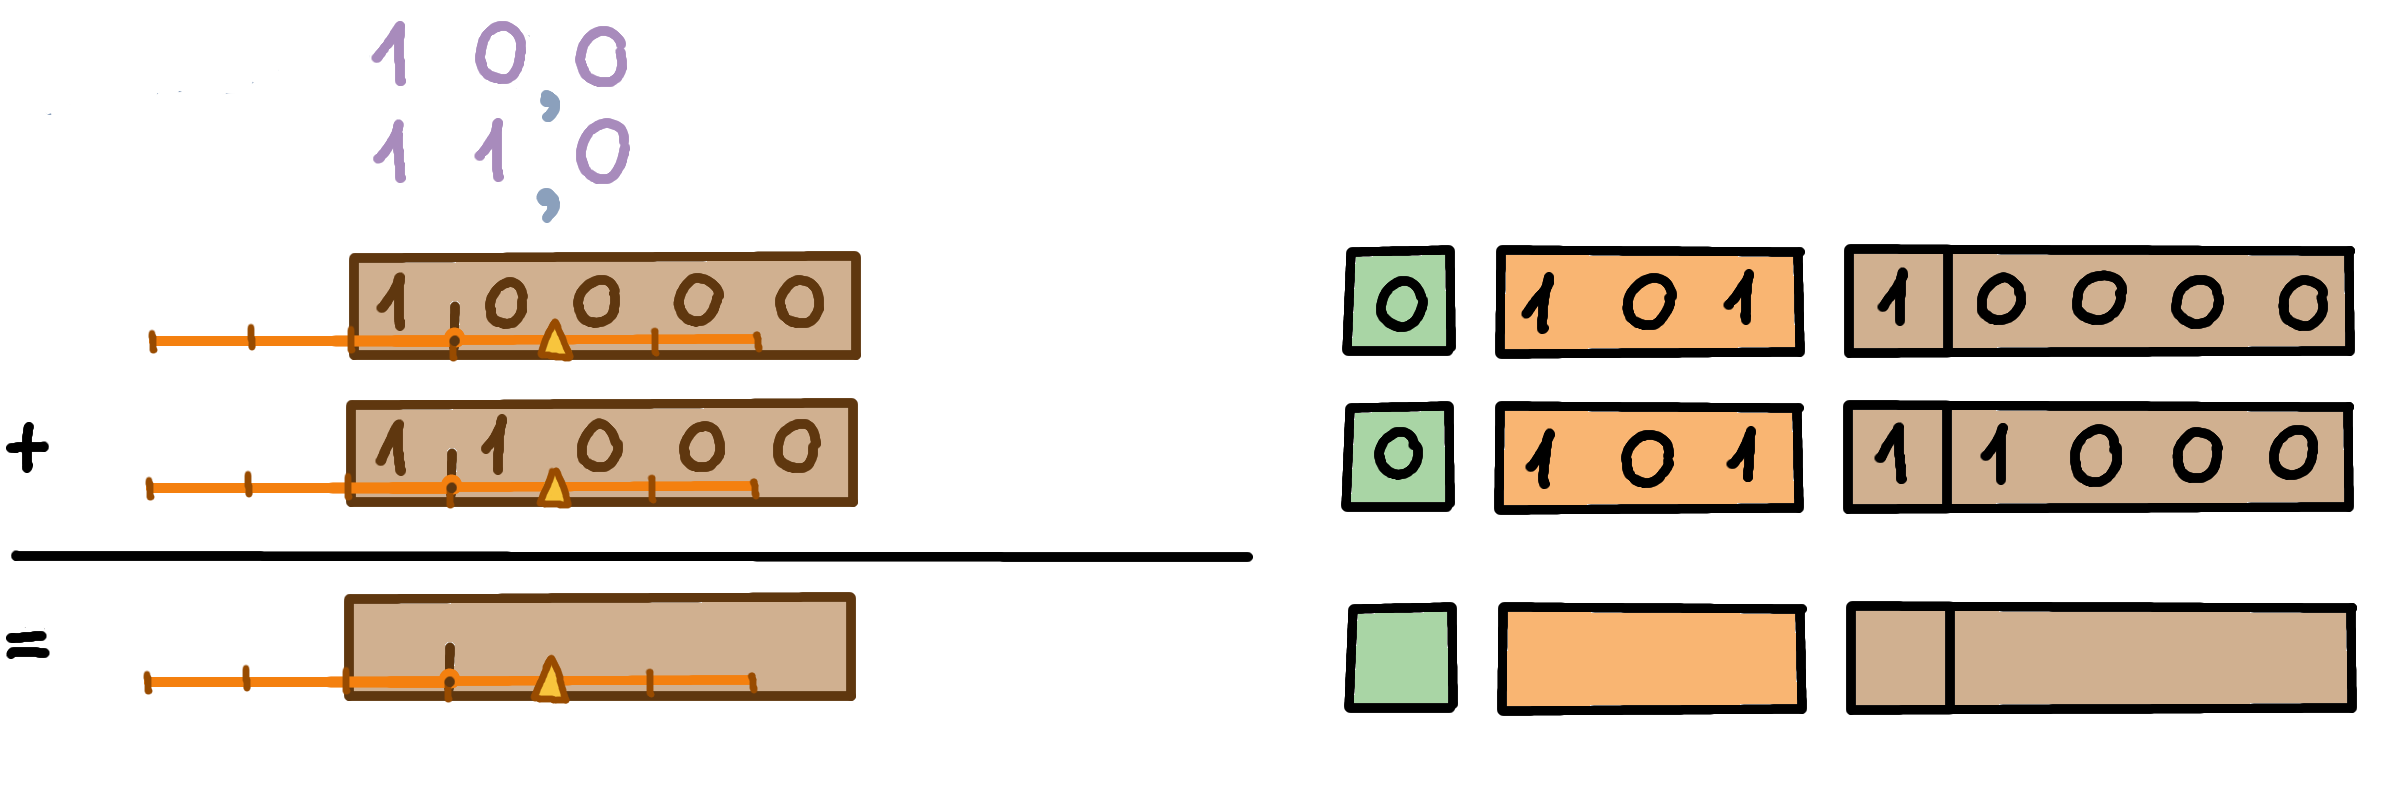
\includegraphics[width=\linewidth]{Pictures/Addition2and3_1.png}
\end{figure}
Die Kasten befinden sich schon untereinander. Wir müssen also nichts verschieben und können sofort losrechnen.
\begin{figure}[H]
\centering
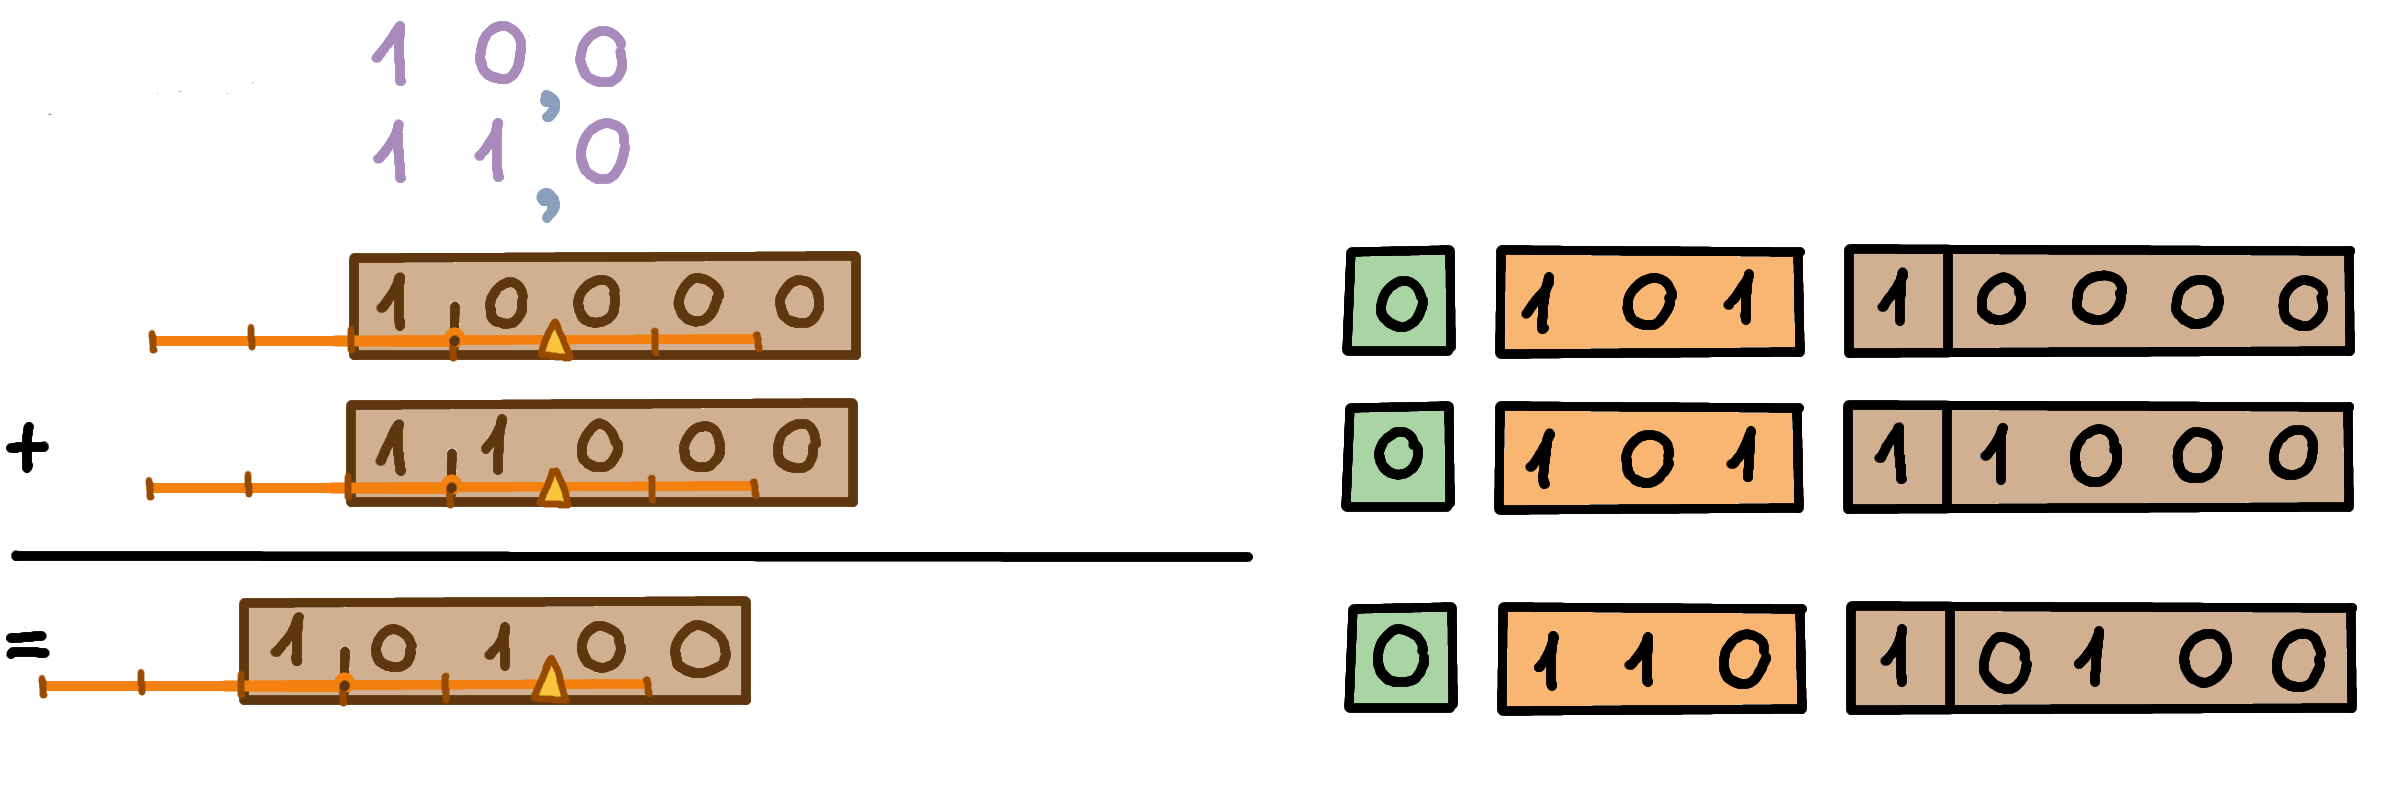
\includegraphics[width=\linewidth]{Pictures/Addition2and3_2.png}
\end{figure}
Beachte, dass der Kasten vom Ergebnis bezüglich den Kasten der Summanden verschoben ist, um die neue signifikante Stelle zu enthalten.

Wir haben ausgerechnet, dass \(2 + 3 = 5\), in der Exponentialschreibweise \(1.0100 \cdot 2^2\).
\end{beispiel}

\begin{aufgabe}\label{addition}
Rechne folgende Summen aus. Die Mantissenlänge beträgt \(5\) Bits, der Exponent geht von \(-3\) bis \(3\). Gebe bitte das Bitmuster und die Exponentialdarstellung des Resultats an.
\begin{enumerate}[(a)]
\item \(5/8 + 3/4\)
\item \(10 + 2.25\)
\item \(17/16 + 2\)
\end{enumerate}
\end{aufgabe}

Die Addition im Fliesskommazahlensystem ist wie gewöhnlich kommutativ, weil wir immer die kleinste Zahl so verschieben, dass ihr Kasten unter dem Kasten der grösseren Zahl steht und dann die Bits in beiden Kasten stellenweise zusammen addieren. In der folgenden Aufgabe werden wir prüfen, ob sie auch assoziativ ist.

\begin{lernaufgabe*}\label{lernaufgabe_assoziativ}
Du wirst jetzt herausfinden, ob die Addition bei den Fliesskommazahlen assoziativ ist. Berechne dazu zwei Mal die gleiche Summe in einem Fliesskommazahlensystem mit Mantissenlänge \(5\) und Exponenten von \(-3\) bis \(3\):
Das erste Mal als \(1/8 + 2/8 + 3/8 + 4/8 + 5/8 + 6/8 + 7/8 + 8/8\) und das zweite Mal als \(8/8 + 7/8 + 6/8 + 5/8 + 4/8 + 3/8 + 2/8 + 1/8\).

Welchen Resultat erwartest du? Sind die zwei Summen gleich oder unterschiedlich? Kannst du daraus folgern, ob Addition assoziativ ist?
Nimm dir Zeit und rechne die zwei Summen tatsächlich aus.
\end{lernaufgabe*}

Die zwei Summen, die du ausgerechnet hast, liefern unterschiedliche Ergebnisse. Die erste liefert den exakten Wert \(4.5\), während bei der zweiten Summe kriegen wir im Fliesskommazahlensystem nur \(4.25\), und das obwohl der exakte Wert dargestellt werden kann. Das passiert, weil man bei den Fliesskommazahlen nur Zahlen der ähnlichen Grössenordnung exakt addieren kann. In der ersten Summe addieren wir die kleineren Summanden am Anfang, wenn die kumulative Summe noch nicht zu gross ist. In der zweiten Summe wächst die kumulative Summe sehr schnell, und irgendwann sind die Summanden zu klein bezüglich der kumulativen Summe, um einen Unterschied zu machen.

Daraus können wir folgern, dass die Addition bei den Fliesskommazahlen nicht assoziativ ist.


\begin{aufgabe}\label{ein_achtel}
Betrachten wir die Summe \(1/8 + 1/8 + 1/8 + \dotsb + 1/8\).
Bei den reellen Zahlen können wir mit solchen Summen auf beliebig grossen Zahlen kommen. Bei den Fliesskommazahlen kann das nicht gehen, weil, wie wir im vorherigen Kapitel gesehen haben, es eine grösste Fliesskommazahl gibt. Aber können wir diese Zahl auch tatsächlich erreichen?

In einem Fliesskommazahlensystem mit Mantissenlänge \(5\) und Exponentenbereich von \(-3\) bis \(3\), was ist die grösste Zahl, die wir erreichen können, wenn wir beliebig viele \(1/8\) zusammen rechnen? Wie viele Summanden brauchen wir, um diese Zahl zu erreichen?
\end{aufgabe}


\subsubsection*{\textcolor{blue-violet}{Teste dich selber}}
\begin{aufgabe}\label{addition_kontrollfragen}
Beantworte folgende Fragen:
\begin{enumerate}[(a)]
\item Warum kann man im Allgemeinen zwei Mantissen nicht stellenweise zusammen addieren?
\item Gregory behauptet, dass der Kasten vom Ergebnis sich immer genau unter dem Kasten der grössten Zahl befindet. Hat er recht? Argumentiere.
\item Hannah behauptet, dass die Addition bei den Fliesskommazahlen nicht kommutativ und nicht assoziativ ist. Hat sie recht? Argumentiere.
\end{enumerate}
\end{aufgabe}

\begin{aufgabe}\label{ameisenkönigin}
Die Ameisenkönigin möchte ausrechnen, wie viele Ameisen braucht sie, um \(10\) Reiskörnchen zu transportieren. Sie weiss, dass eine Ameise allein \(1/4\) Reiskorn transportiert. Die Ameisenkönigin hat dazu folgendes Programm geschrieben.
\begin{lstlisting}[language=Python, caption={Programm von der Ameisenkönigin}]
def nof_ameisen():
    sum = 0.0
    i = 0
    while node != 10.0:
    	i += 1
       sum += 0.25
    return i
\end{lstlisting}
Die Ameisencomputer arbeiten mit Fliesskommazahlen mit Mantissenlänge \(5\) und Exponenten zwischen \(-3\) und \(3\).
Kann die Ameisenkönigin mit diesem Programm die gewünschte Anzahl Ameisen herausfinden? Falls ja, wie viele Ameisen braucht sie, um 10 Reiskörnchen zu transportieren laut diesem Programm? Falls nein, was ist die maximale Summe, die das Programm erreichen kann?
\end{aufgabe}
\newpage

\section{Zusammenfassung}
Wir haben gesehen, wie man im Computer reelle Zahlen approximiert. Da wir eine endliche Darstellung verwenden, gibt es eine endliche Anzahl Zahlen, die wir darstellen können. Es gibt eine grösste und eine kleinste positive Zahl.

Die grösste positive Zahl kriegen wir, wenn wir in der Mantisse nur Einser schreiben und den Exponent so weit wie möglich hochdrehen. Die kleinste positive Zahl kriegen wir, wenn wir in der Mantisse eine führende Eins schreiben und sonst nur Nullen und den kleinstmöglichen Exponenten wählen.

Wir haben gesehen, dass der kleinste Abstand zwischen zwei darstellbaren Zahlen wächst, wenn die Zahlen wachsen.

Wir haben gelernt, wie man zwei Zahlen zusammen addiert. Wir haben gesehen, dass zwei darstellbare Zahlen sich nicht immer exakt addieren lassen. Wir haben auch gesehen, dass es einen Unterschied macht, in welcher Reihenfolge man Berechnungen ausführt. Die Addition ist bei Fliesskommazahlen kommutativ aber nicht assoziativ.

Die Fliesskommazahlen sind eine mächtige Darstellung, die mit wenig Bits sehr unterschiedliche Zahlen speichern kann. Das hat aber auch seine Grenzen. Wir müssen in Kauf nehmen, dass die Resultate der Berechnungen nicht immer 100\% genau sind.

\newpage

\nocite{*}
\bibliographystyle{plain}
\bibliography{refs}
\newpage

\section{Beispiellösungen}
\subsection{Einführung}
\paragraph{Aufgabe \ref{einleitung-vom-kasten-nach-zahl}}
Das Vorzeichen ist positiv. Die Mantisse übernehmen wir aus dem Kasten. Die Kodierung vom Exponenten können wir am Seil ablesen. Den Exponenten bestimmen wir, indem wir die \texttt{100} auf dem Seil als \(0\) interpretieren und die Stellen zwischen der Null und der Markierung zählen. In diesem Fall sind es \(-2\) Stellen.
\begin{figure}[H]
\centering
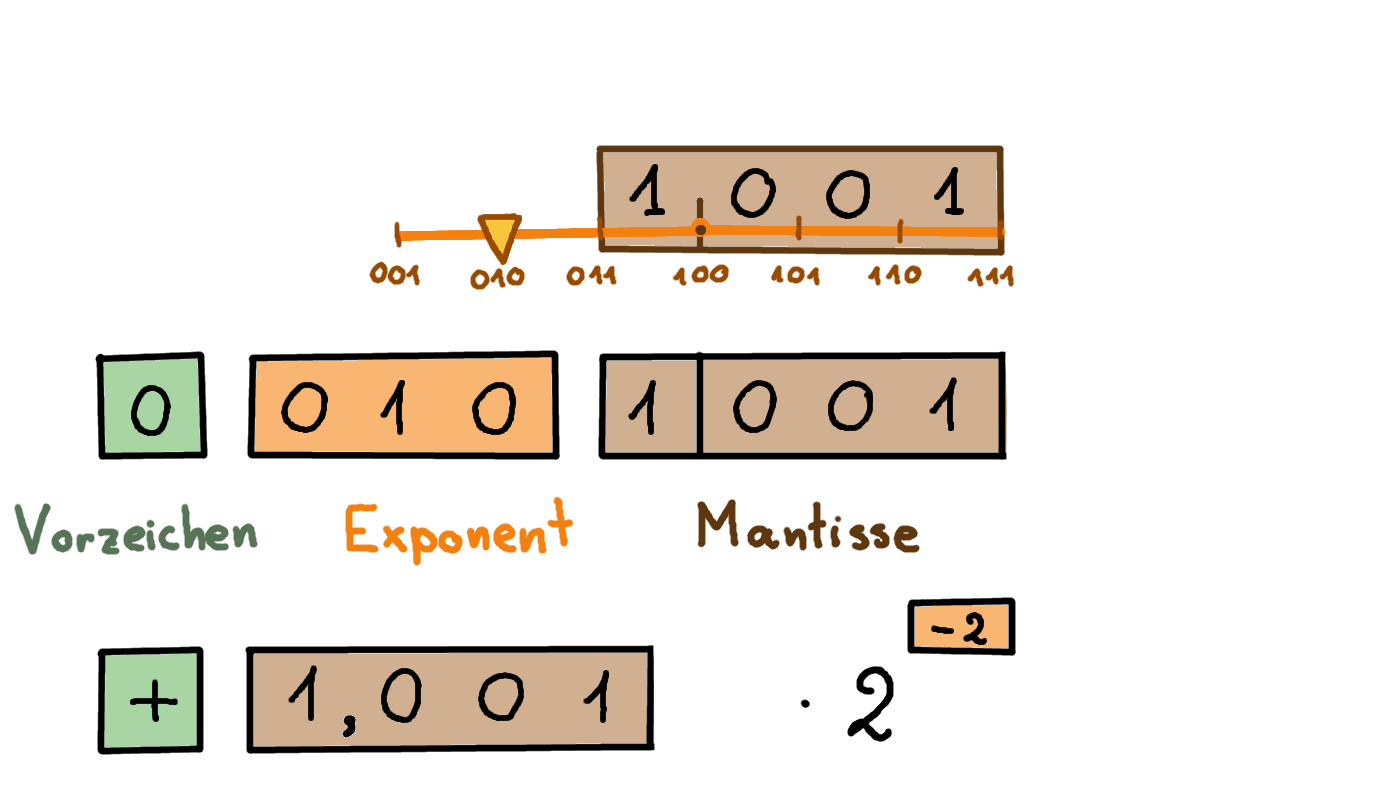
\includegraphics[width=0.8\linewidth]{Pictures/Einleitung_from_Kasten_Loesung.png} 
Den Dezimalwert berechenen wir, indem wir \((-1)^0 \cdot 1.001 \cdot 2^{-2} = 0.01001\) nach Dezimal konvertieren. In diesem Fall erhalten wir \(1/4 + 1/32 = 9/32\).
\end{figure}

\subsection{Fliesskommazahlen}

\paragraph{Aufgabe \ref{kleinsteZahl-5-3}}
Wir konstruieren die kleinste positive Zahl im Fliesskommazahlensystem mit Mantissenlänge \(5\) und Exponenten von \(-3\) bis \(3\).

Als erstes platzieren wir den Kasten. Damit die Zahl möglichst klein wird, muss der Kasten nach rechts möglichst weit weg vom Komma stehen. Wir haben aber eine Einschränkung: Das Seil muss immer mit dem Komma verbunden bleiben.
\begin{figure}[H]
\centering
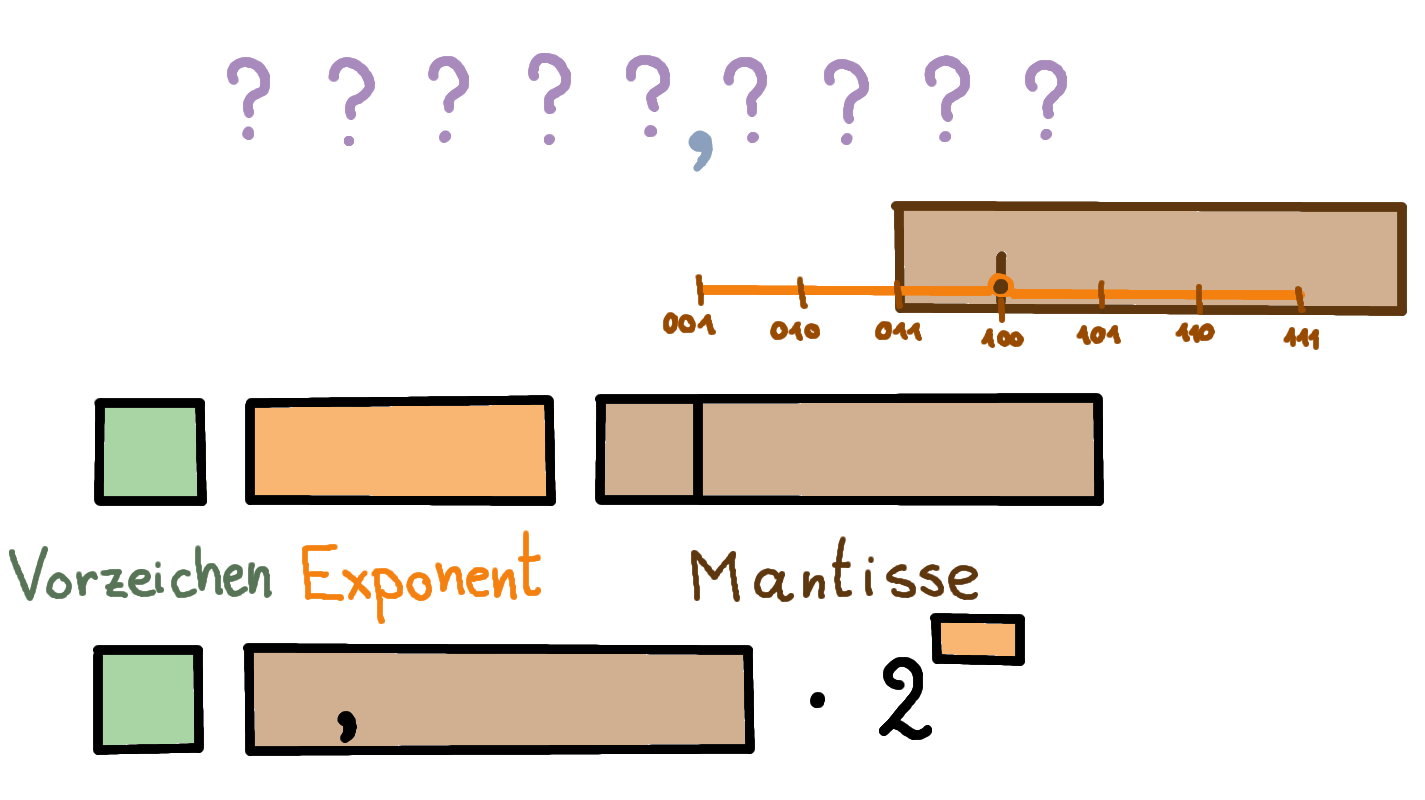
\includegraphics[width=0.85\linewidth]{Pictures/kleinsteZahl1.png}
\end{figure}
Der Exponent muss also möglichst klein sein.

Was ist mit der Mantisse? Sicher muss eine Eins an der ersten Stelle stehen.
\begin{figure}[H]
\centering
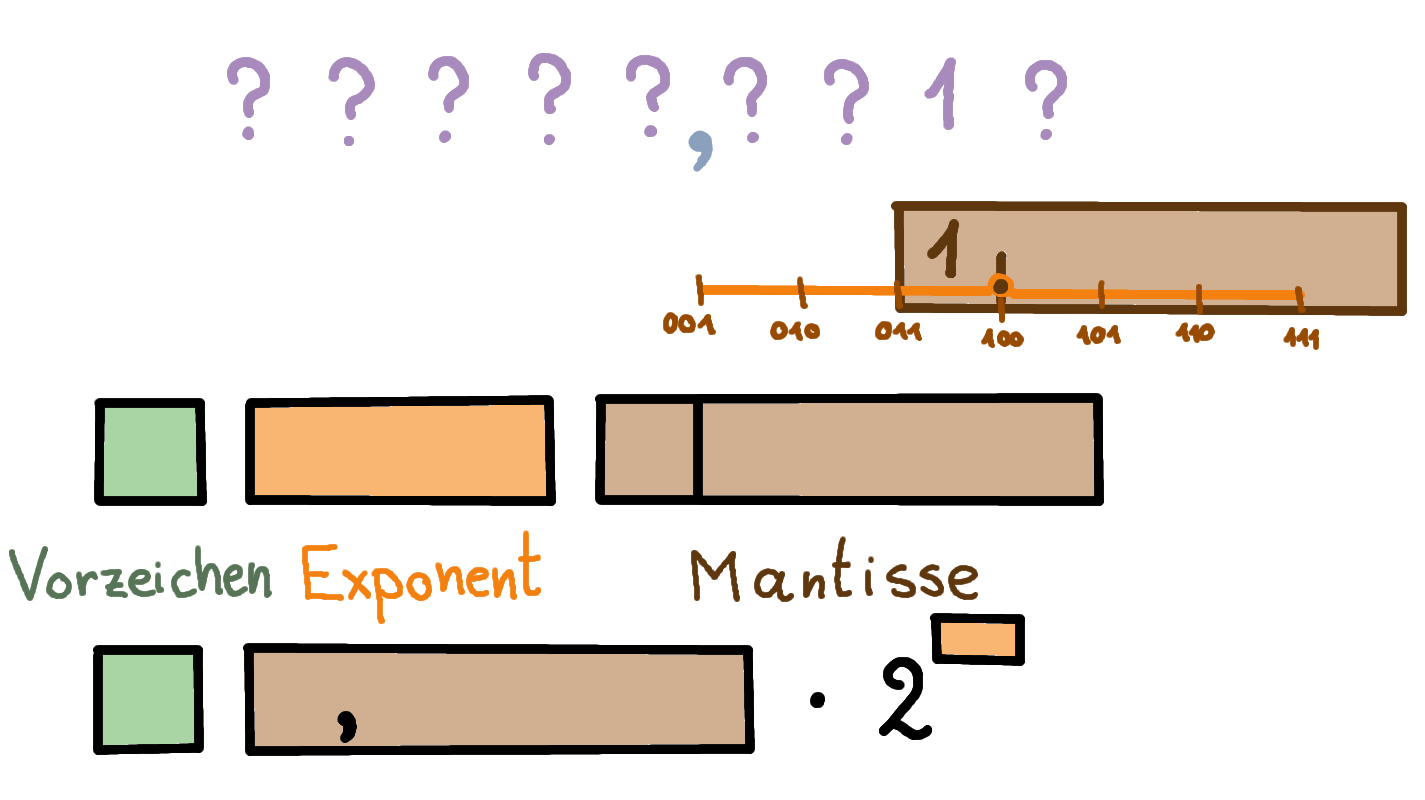
\includegraphics[width=0.85\linewidth]{Pictures/kleinsteZahl2.png}
\end{figure}

Damit die Mantisse möglichst klein wird, müssen wir so viele Stellen wie möglich auf Null setzen.
\begin{figure}[H]
\centering
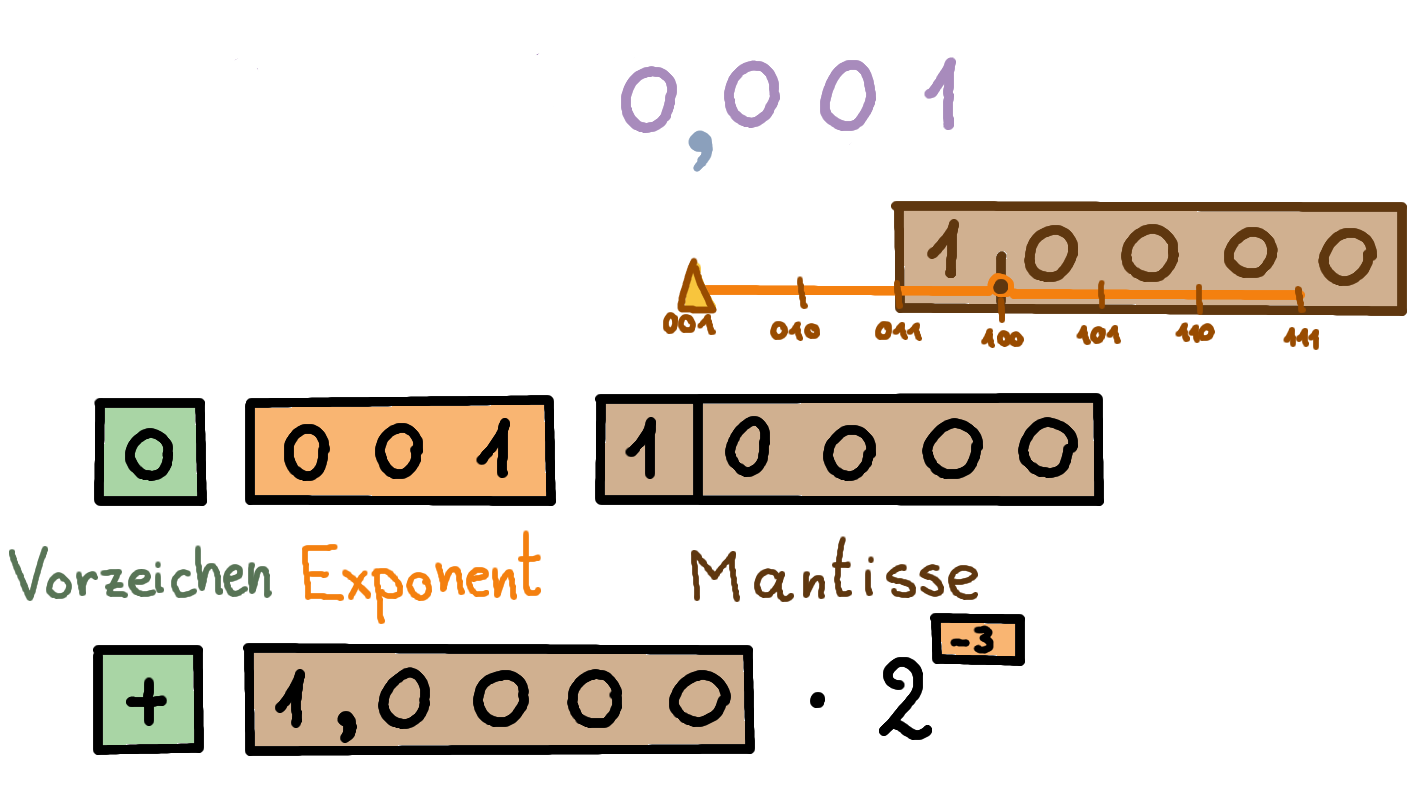
\includegraphics[width=0.85\linewidth]{Pictures/kleinsteZahl3.png}
\end{figure}

Die kleinste darstellbare Zahl in diesem Fliesskommazahlensystem ist also \(1/8\).

\paragraph{Aufgabe \ref{groesste-kleinste-4-3}}
Die grösste positive darstellbare Zahl in einem Fliesskommazahlensystem mit Mantissenlänge \(4\) und Exponent zwischen \(-3\) und \(3\) ist \(15\). Das ist nicht viel kleiner als \(15.5\), die grösste positive darstellbare Zahl in einem Fliesskommazahlensystem mit einem Bit mehr für die Mantisse.
\begin{figure}[H]
\centering
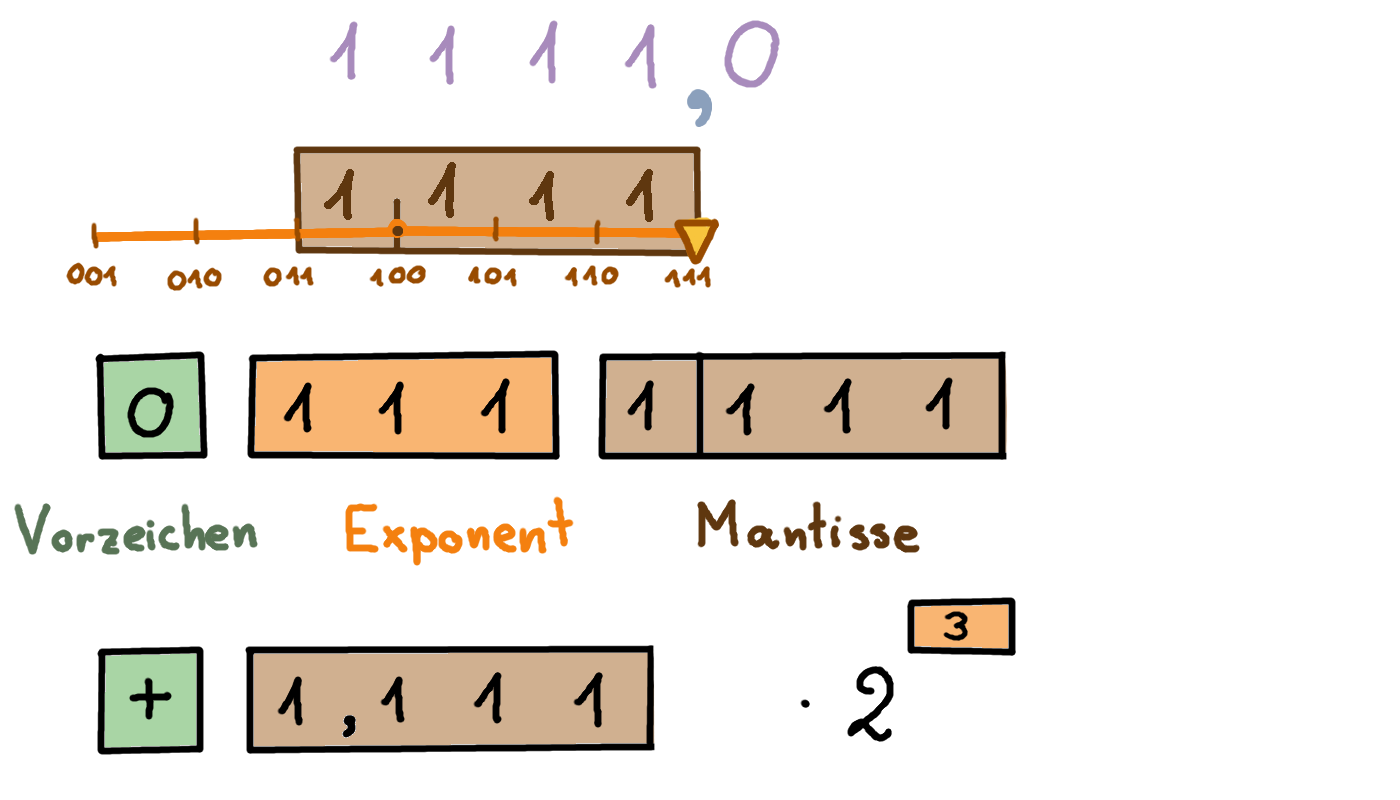
\includegraphics[width=0.85\linewidth]{Pictures/groessteZahl-4-3.png}
\end{figure}

Die kleinste positive darstellbare Zahl in einem Fliesskommazahlensystem mit Mantissenlänge \(4\) und Exponent zwischen \(-3\) und \(3\) ist auch \(1/8\), genau wie die kleinste positive darstellbare Zahl in einem Fliesskommazahlensystem mit einem Bit mehr für die Mantisse.
\begin{figure}[H]
\centering
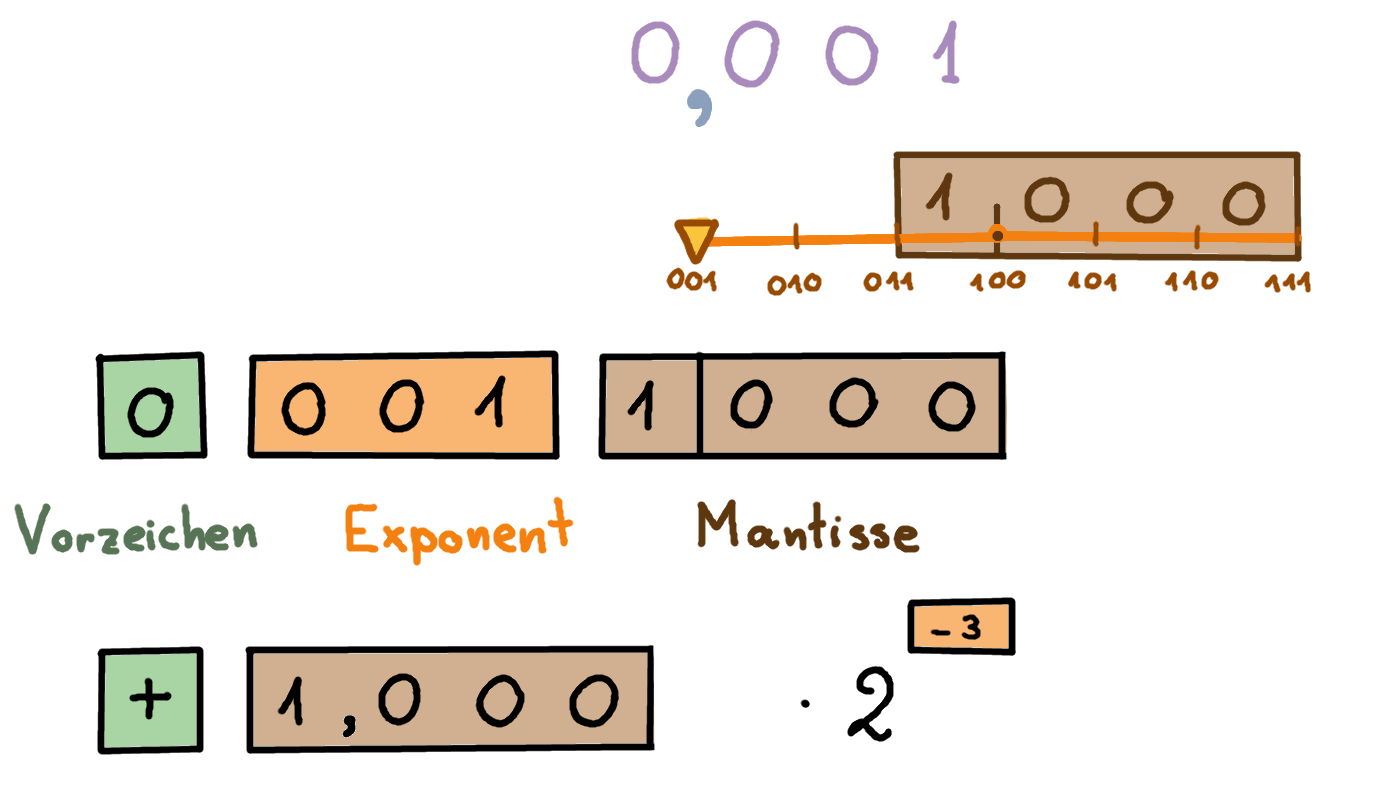
\includegraphics[width=0.85\linewidth]{Pictures/kleinsteZahl-4-3.png}
\end{figure}

Wie wir sehen, die Länge der Mantisse scheint wenig Einfluss auf die grösste und kleinste positive darstellbare Zahlen zu haben.

\paragraph{Aufgabe \ref{groesste-kleinste-5-2}}
\begin{enumerate}[(a)]
\item Der Exponent liegt zwischen \(-1\) und \(1\) und die mögliche Kodierungen sind \texttt{01, 10, 11}.
\item Die Erwartung ist, dass die grösste positive darstellbare Zahl deutlich kleiner wird, weil das Seil viel kürzer ist, und wir den Kasten nicht mehr so weit nach links ziehen können, wie im Fliesskommazahlensystem mit \(3\) Bits für den Exponenten. Analog, die kleinste positive darstellbare Zahl wird deutlich grösser.
\item Die grösste positive darstellbare Zahl in diesem System ist \(3+7/8 = 31/8\). Wie erwartet, das ist viel grösser als in einem Fliesskommazahlensystem mit einem Bit mehr für den Exponenten.
\begin{figure}[H]
\centering
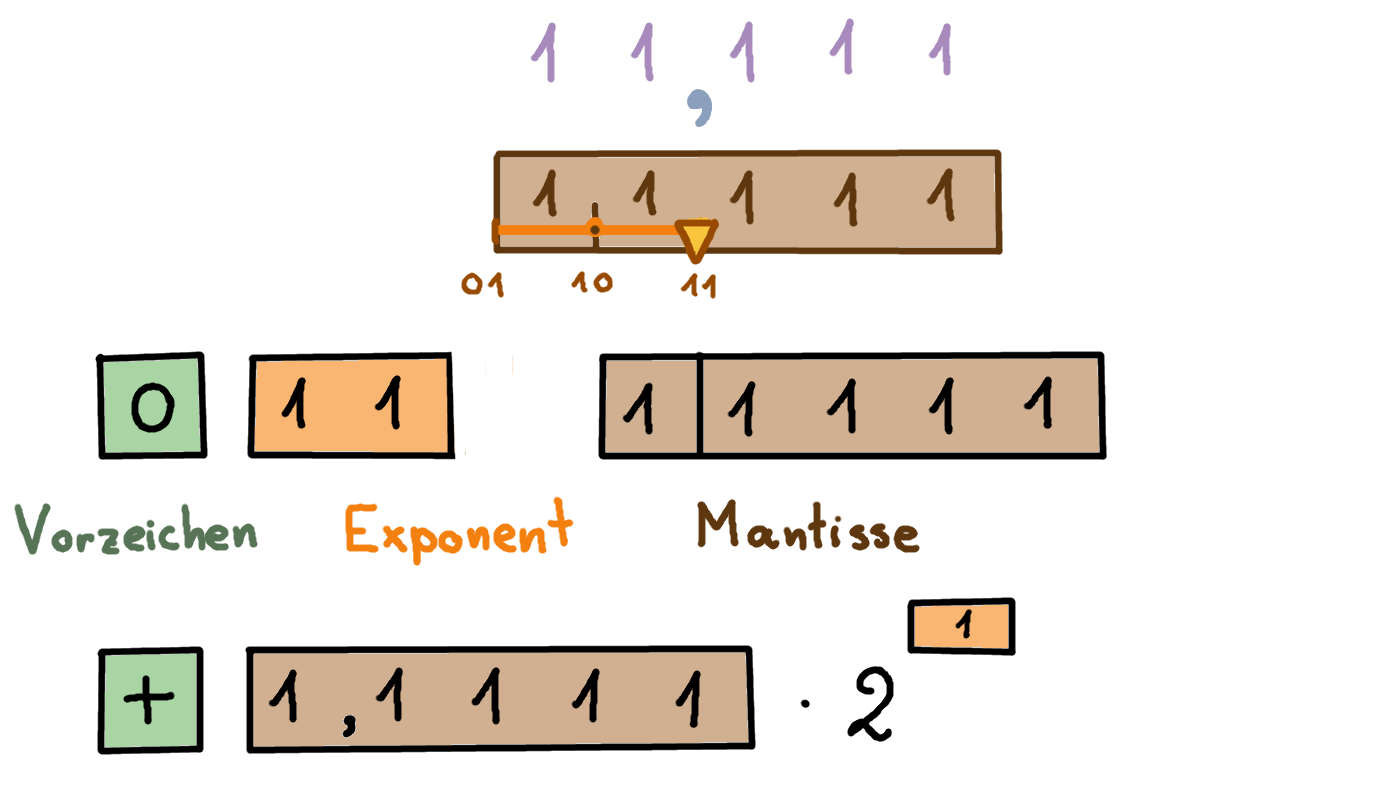
\includegraphics[width=0.85\linewidth]{Pictures/groessteZahl-5-2.png}
\end{figure}

Die kleinste positive darstellbare Zahl in diesem System ist \(0.5\). Das ist viel grösser als in einem Fliesskommazahlensystem mit einem Bit mehr für den Exponenten.
\begin{figure}[H]
\centering
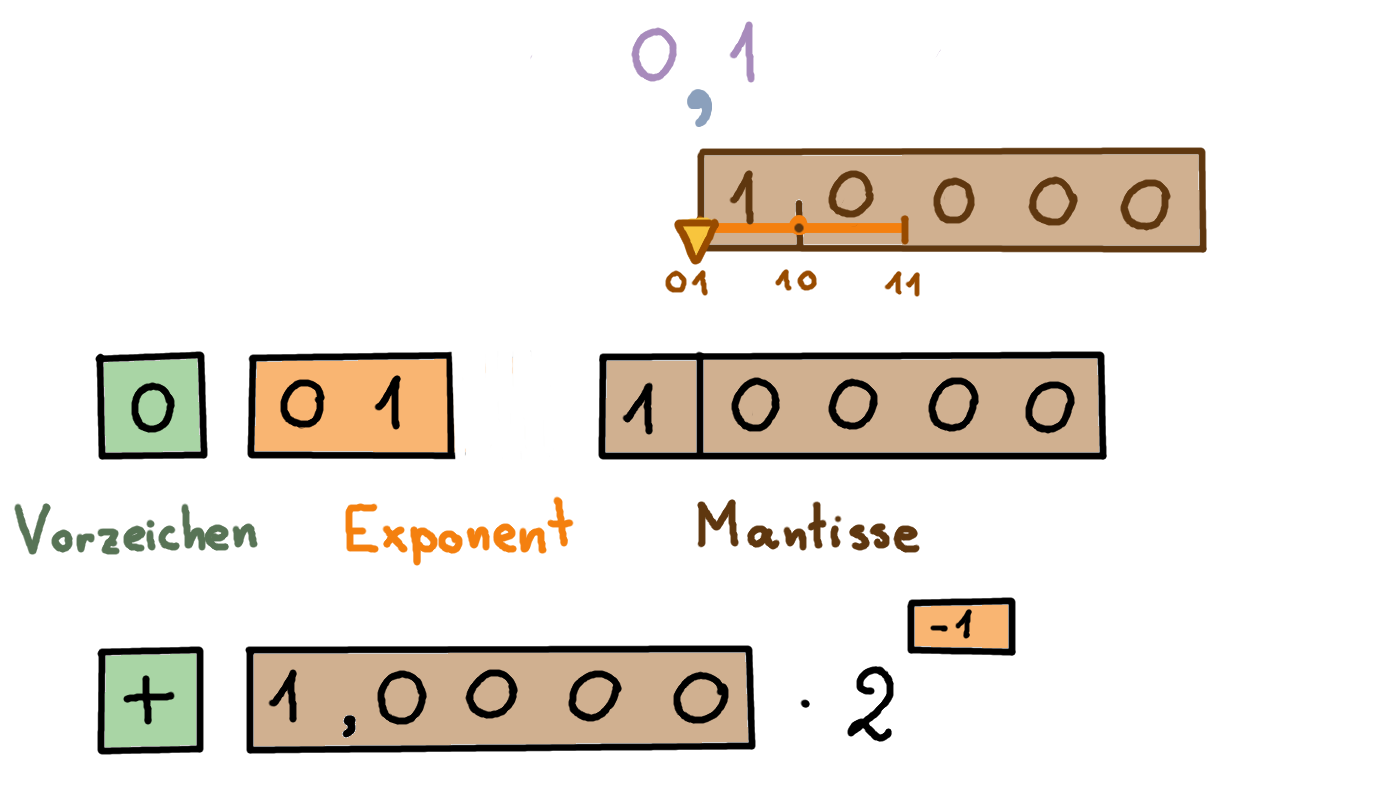
\includegraphics[width=0.85\linewidth]{Pictures/kleinsteZahl-5-2.png}
\end{figure}

\end{enumerate}


\paragraph{Aufgabe \ref{groesste-kleinste-allgemein}}

Im Allgemeinen für einen Fliesskommazahlensystem mit Mantissenlänge \(m\) und Exponenten zwischen \(e_{min}\) und \(e_{max}\) findet man die grösste und kleinste positive Zahlen wie folgt.

Für die grösste positive Zahl wählt man den grösstmöglichen Exponenten \(e_{max}\) und die grösstmögliche Mantisse \(1.111 \ldots 111\). In der Exponentialschreibweise ist die grösste Zahl also 
\[1.1111111 \ldots 111 \cdot 2^{e_{max}}\]
und hat das Bitmuster \texttt{0 1111...111 (1)111111...111}.

Für die kleinste positive Zahl wählt man den kleinsten möglichen Exponenten \(e_{min}\) und die kleinste mögliche Mantisse. Beachte, dass die Mantisse immer mit einer Eins starten muss. Die kleinste mögliche Mantisse ist deswegen \(1.0000 \ldots 000\). In der Exonentialschreibweise ist die kleinste Zahl also
\[1.0000000 \ldots 000 \cdot 2^{e_{min}}\]
und hat das Bitmuster \texttt{0 0000...001 (1)00000000...000}.
%--------------------------------

\paragraph{Aufgabe \ref{nachbarn-vorherige}}
Die nächstkleinste, oder vorherige, darstellbare Zahl finden wir, indem wir die Mantisse kleiner zu machen versuchen. Da die Mantisse von \(1\) die kleinste mögliche Mantisse ist, müssen wir den Exponenten um Eins zurücksetzen und die grösstmögliche Mantisse wählen.

\begin{figure}[H]
\centering
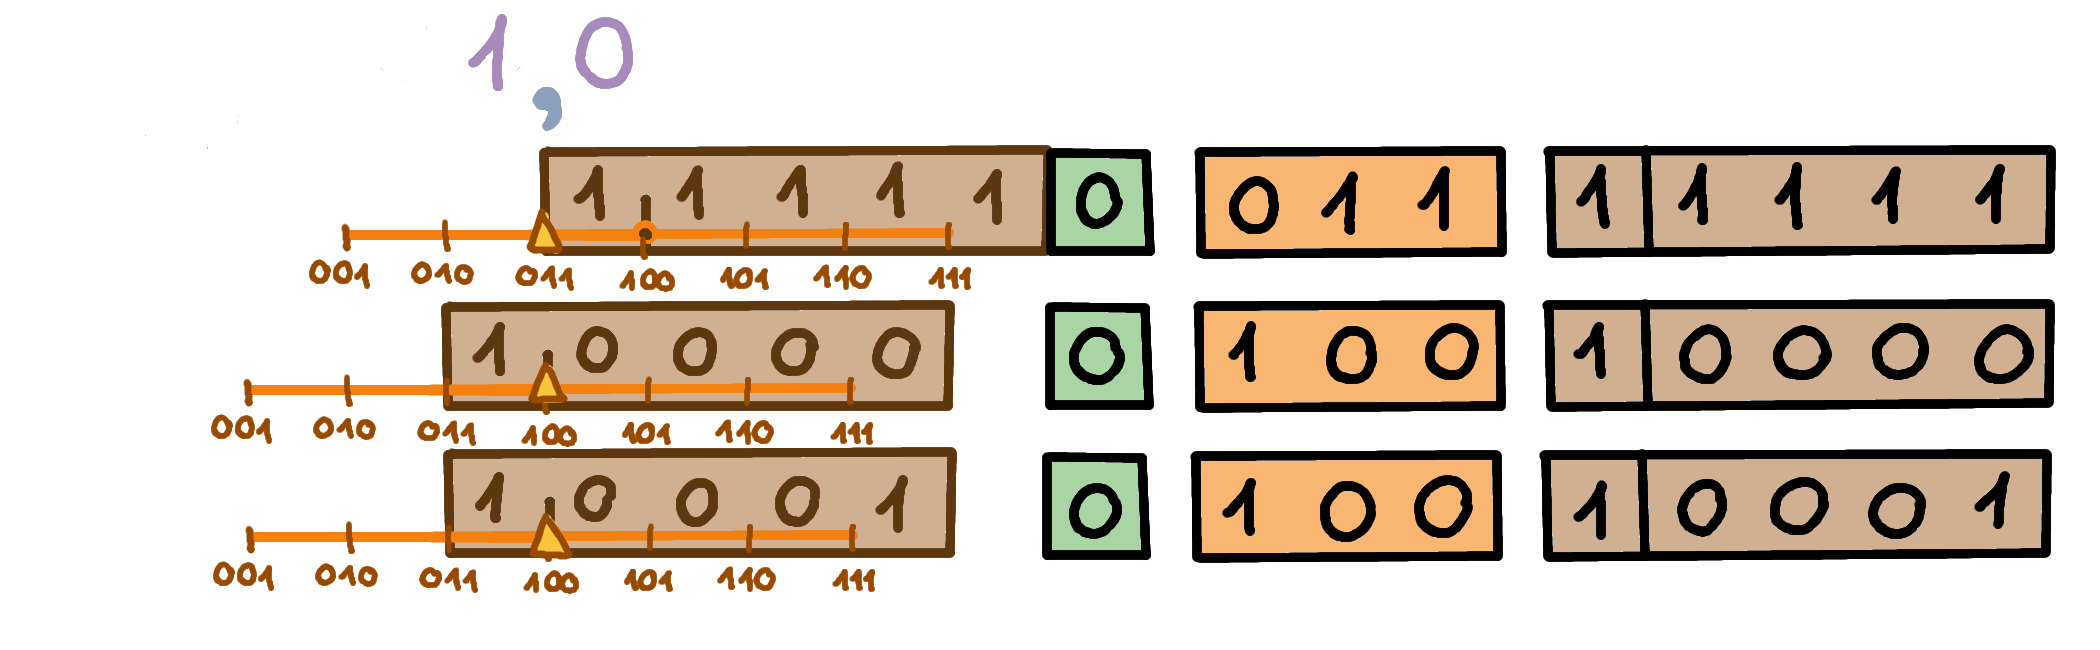
\includegraphics[width=\linewidth]{Pictures/Nachbarn1_P.png} 
\end{figure}
Die vorherige Zahl ist also \(31/32\).

Beachte, dass der Abstand zur nächsten und vorherigen darstellbaren Zahlen in diesem Fall nicht symmetrisch ist: die nächste Zahl ist \(1/16\) entfernt, während die vorherige nur \(1/32\).

\paragraph{Aufgabe \ref{nachbarn}}

\begin{enumerate}[(a)]
\item Die Nachbarn von \(2\) sind \(31/16\) und \(17/8\).
\begin{figure}[H]
\centering
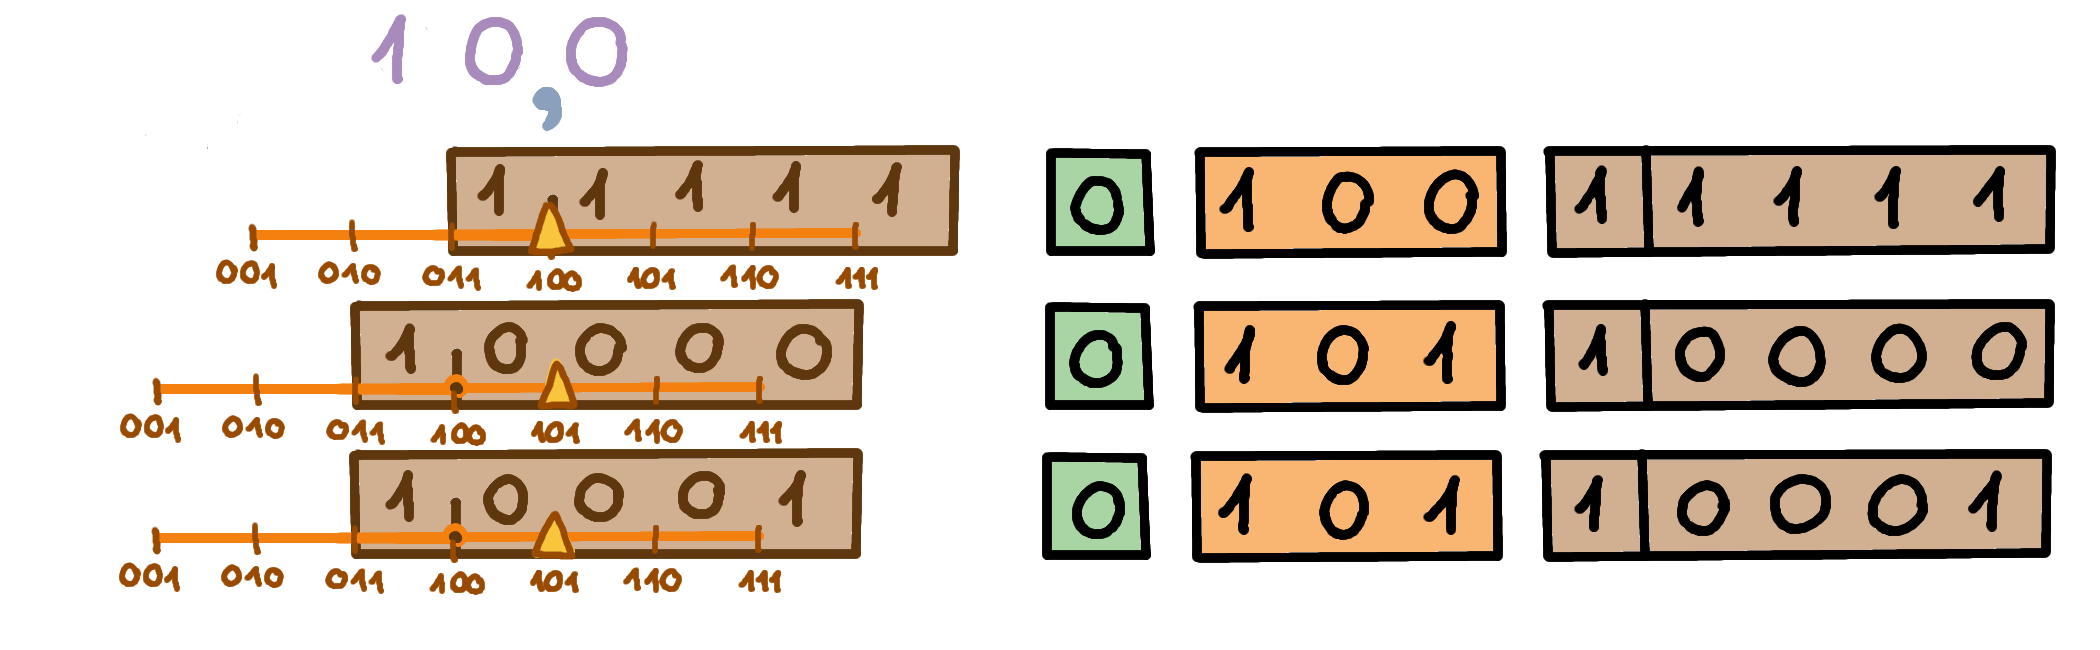
\includegraphics[width=\linewidth]{Pictures/Nachbarn2.png}
\end{figure}

\item Die Nachbarn von \(3\) sind \(23/8\) und \(25/8\).
\begin{figure}[H]
\centering
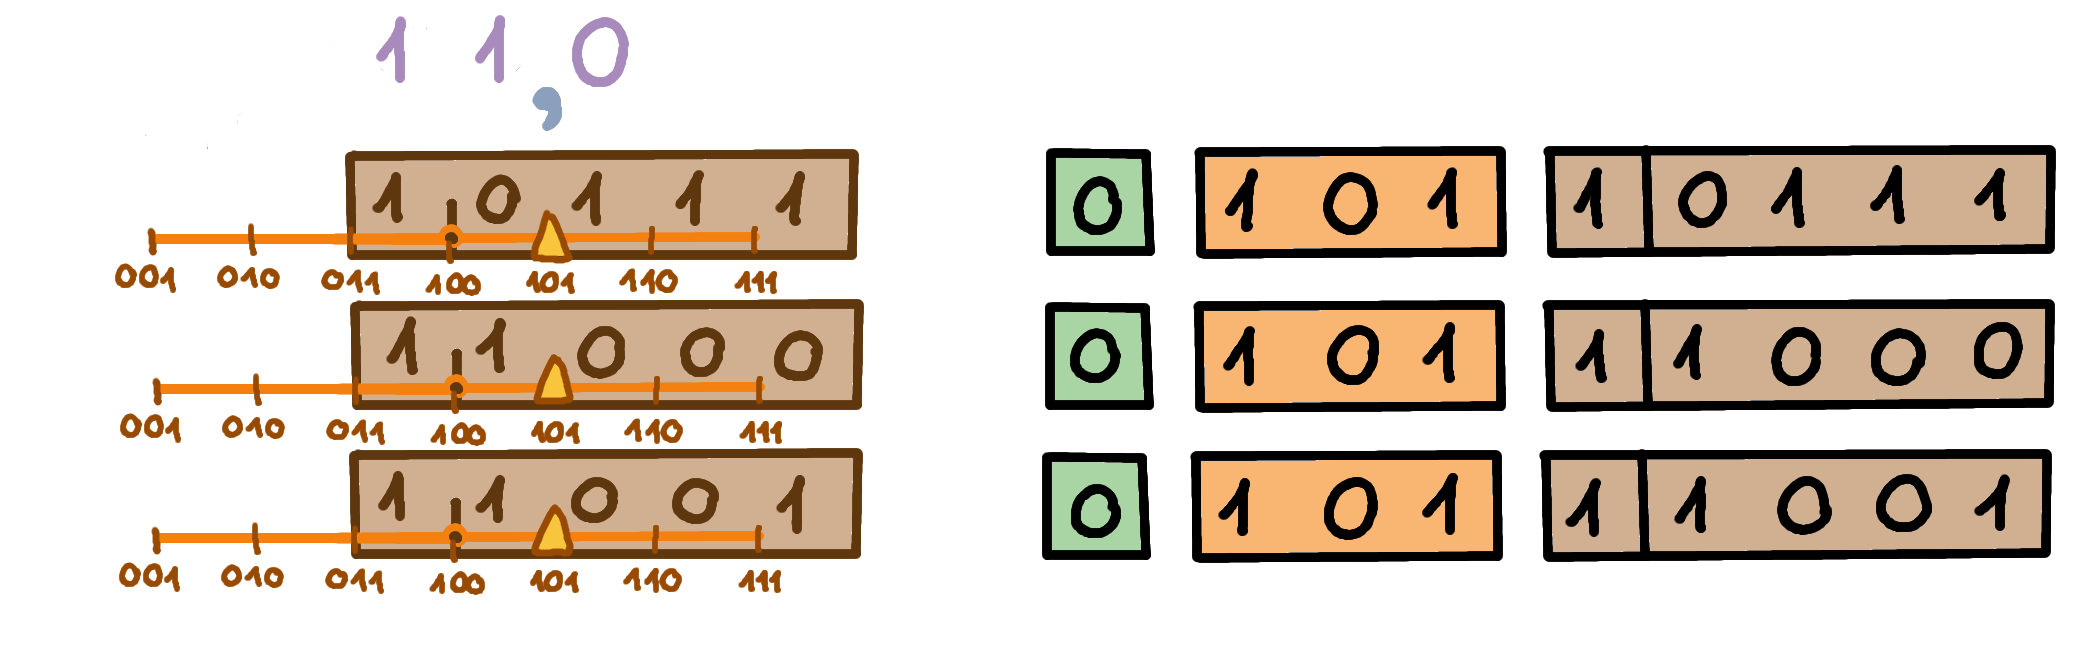
\includegraphics[width=\linewidth]{Pictures/Nachbarn3.png}
\end{figure}

\item Die Nachbarn von \(4\) sind \(31/8\) und \(17/4\).
\begin{figure}[H]
\centering
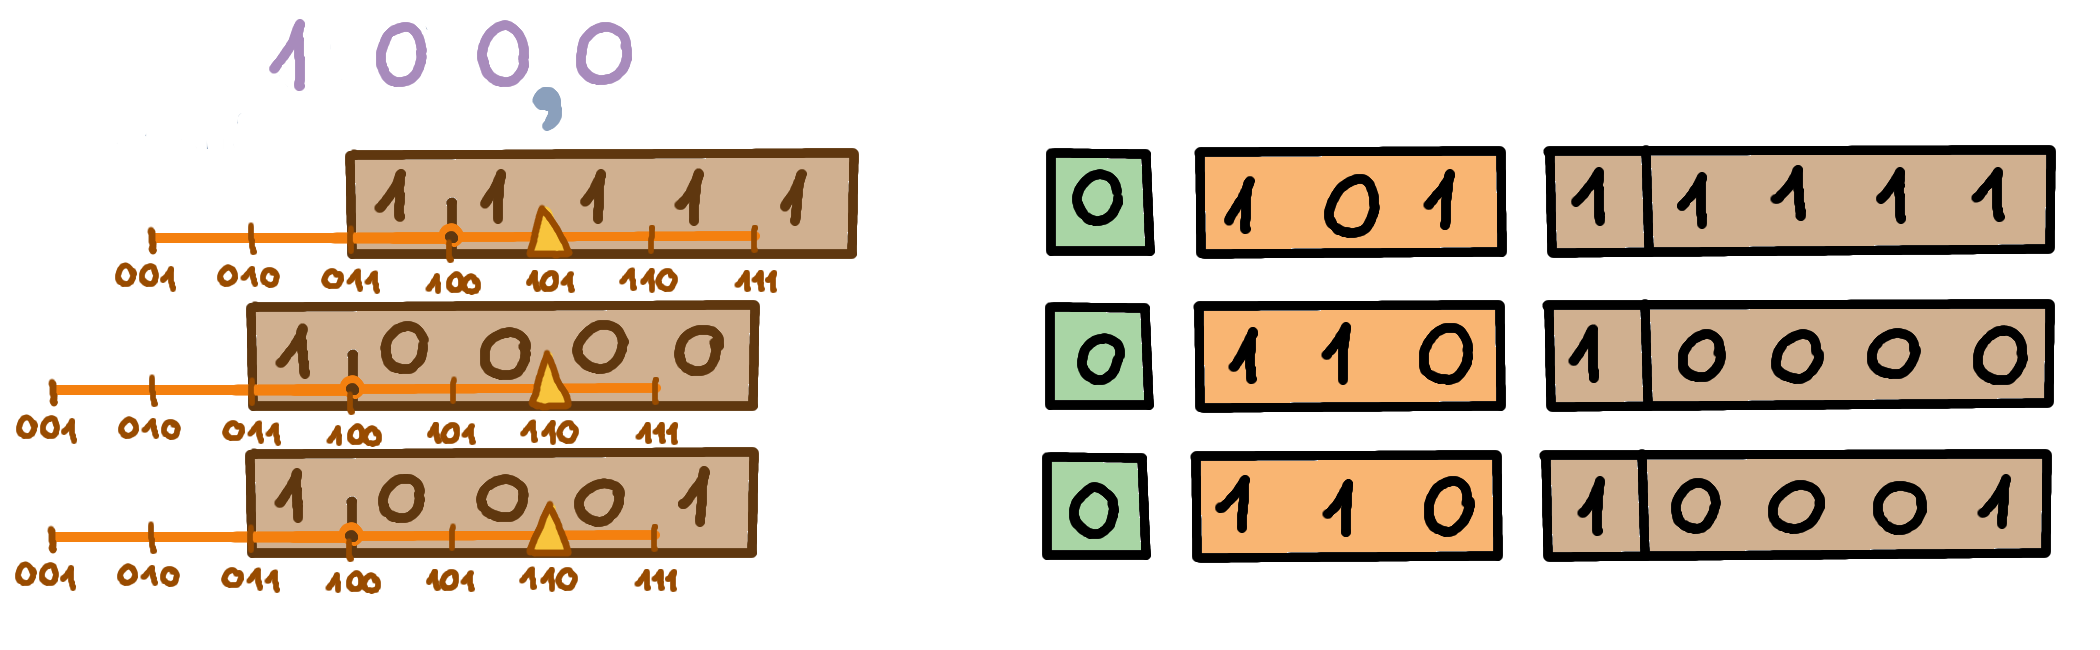
\includegraphics[width=\linewidth]{Pictures/Nachbarn4.png}

Die positive darstellbare Zahlen sind auf dem Zahlenstrahl nicht gleichverteilt.
\end{figure}

\end{enumerate}

\paragraph{Aufgabe \ref{nachbarn-laenge}}
\begin{enumerate}[(a)]
\item Im Fliesskommazahlensystem mit Mantissenlänge \(4\) und Exponent zwischen \(-3\) und \(3\) sind die Nachbarn von \(1\): \(15/16\) und \(9/8\).
\begin{figure}[H]
\centering
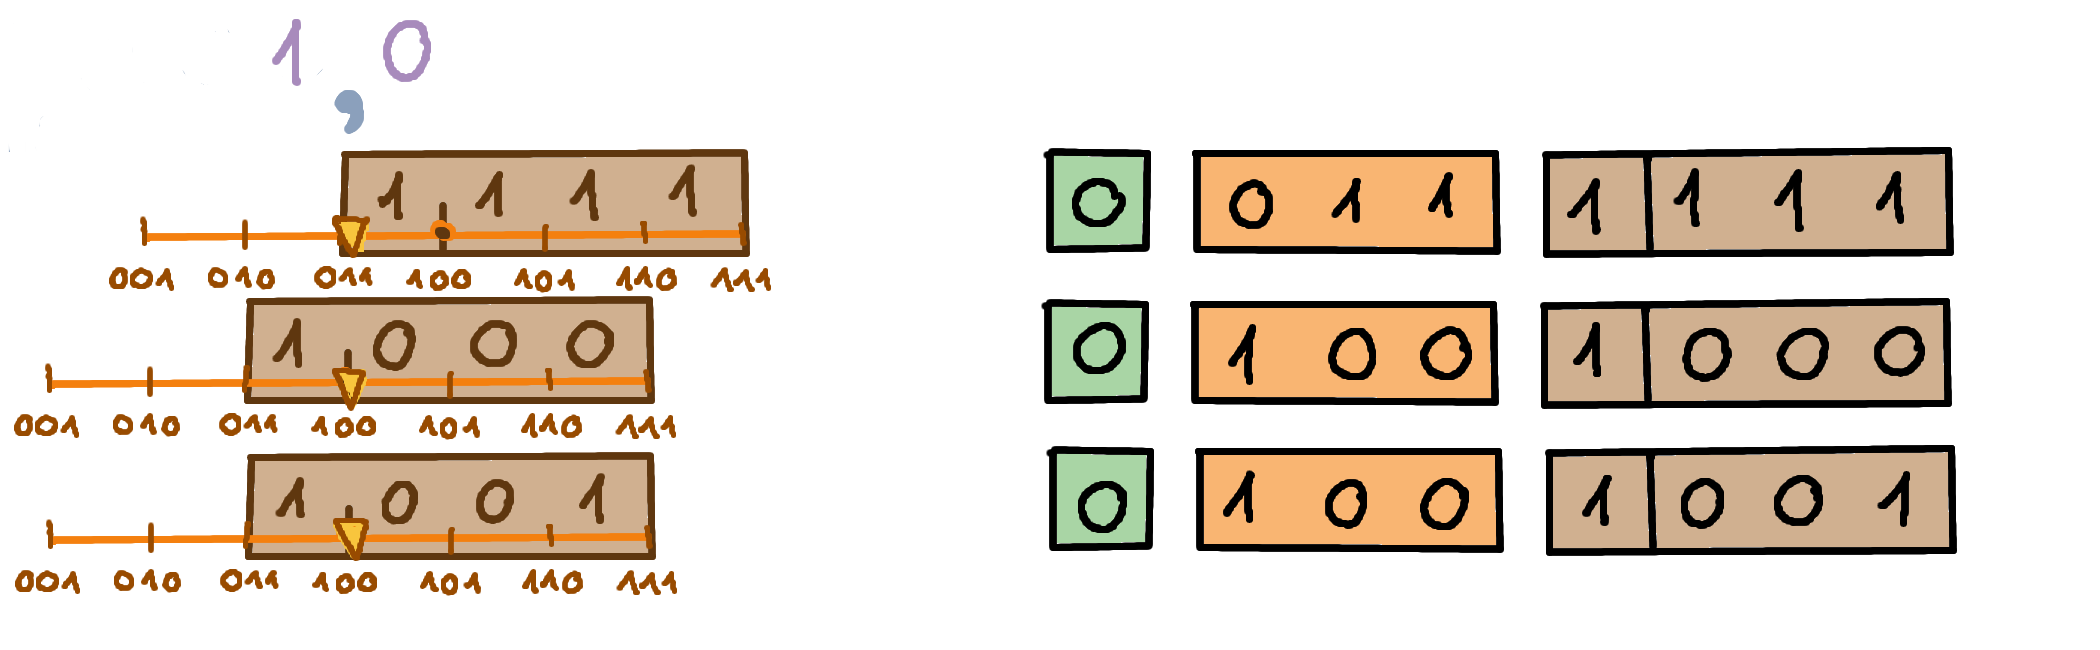
\includegraphics[width=\linewidth]{Pictures/Nachbarn1-4-3-Loesung.png}
\end{figure}

\item Im Fliesskommazahlensystem mit Mantissenlänge \(5\) und Exponent zwischen \(-1\) und \(1\) sind die Nachbarn von \(1\): \(31/32\) und \(17/16\).
\begin{figure}[H]
\centering
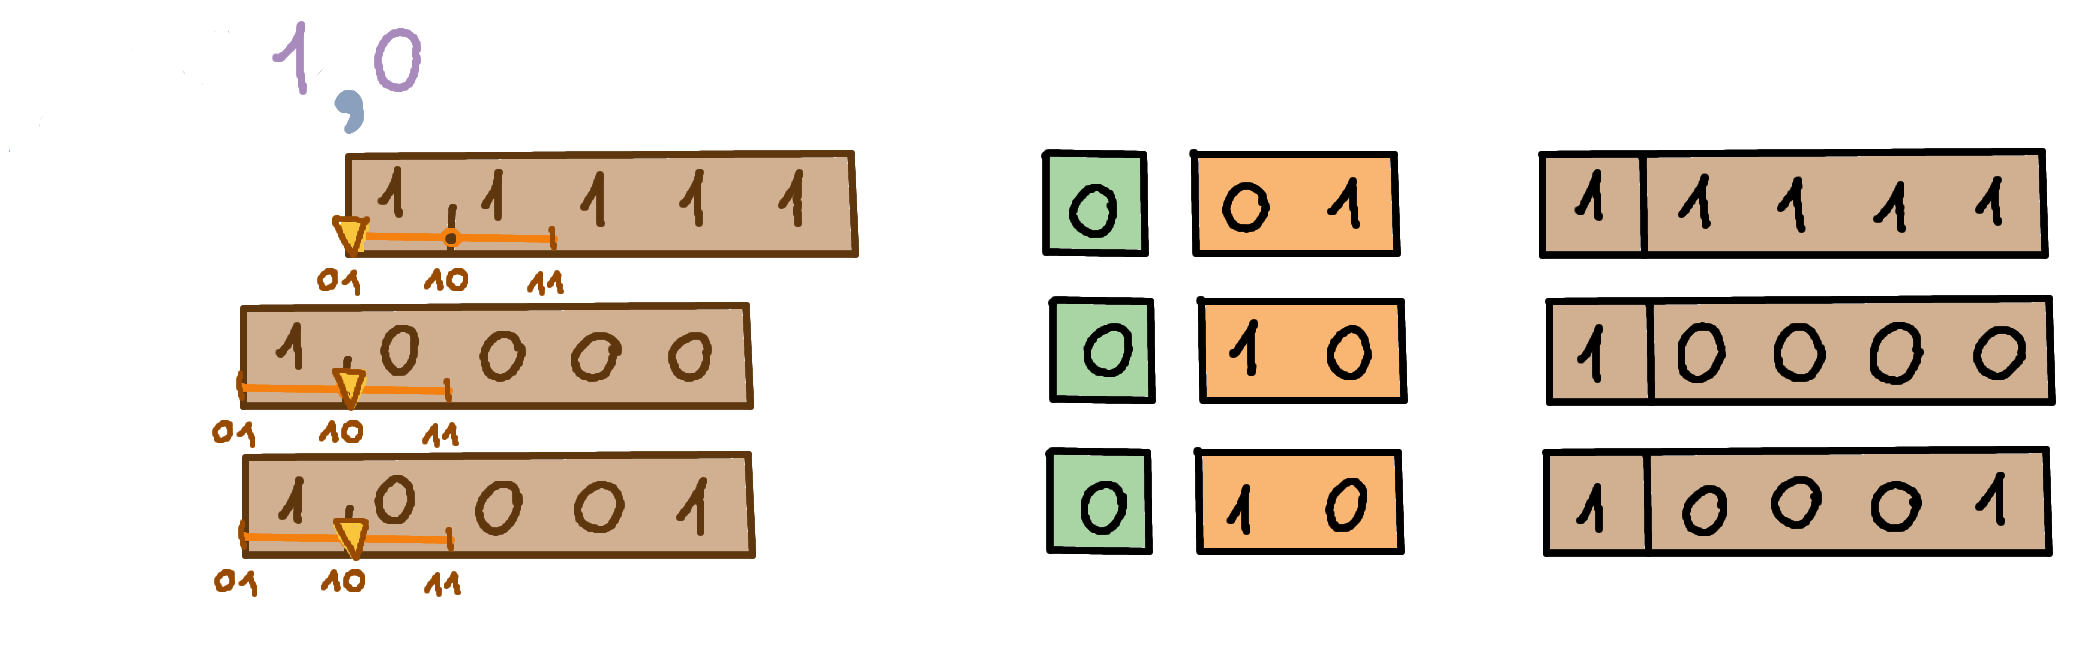
\includegraphics[width=\linewidth]{Pictures/Nachbarn1-5-2-Loesung.png}
\end{figure}

\item Die Länge der Mantisse beeinflusst den Abstand zwischen darstellbaren Zahlen stärker als die Länge der Exponentenkodierung. Wenn der Kasten grösser ist, gibt es mehr Platz für signifikante Stellen und Zahlen können genauer approximiert werden. Das führt dazu, dass der Abstand zwischen darstellbaren Zahlen kleiner wird.
\end{enumerate}

%--------------------------------

\paragraph{Aufgabe \ref{fliesskommazahlen_kontrollfragen}}
\begin{enumerate}[(a)]
\item Nein, es gibt unendlich viele reelle Zahlen und endlich viele Fliesskommazahlen.
\item Ja, die grösste Zahl ist \(1.1111 \ldots 111 \cdot 2^{e_{max}}\).
\item Ja, die kleinste Zahl ist \(1.0000 \ldots 000 \cdot 2^{e_{min}}\).
\item Die Länge der Exponentenkodierung beeinflusst den Bereich stärker als die Mantissenlänge. Wenn das Seil länger ist, kann man den Kasten weiter weg vom Komma platzieren und viel grössere oder kleinere Zahlen darstellen.
\item Zum Beispiel, die Zahl \(2.25\) lässt sich in diesem System nicht exakt darstellen. In der Exponentialschreibweise diese Zahl ist \(1.001 \cdot 2^{1}\). Um diese Zahl exakt zu speichern bräuchten wir \(4\) Bits für die Mantisse, wir haben aber nur \(3\).
\item Nein, die darstellbare Fliesskommazahlen sind nicht gleichverteilt. Die kleineren stehen dichter beieinander, weil bei kleineren Zahlen die letzte Stelle der Mantisse weniger Wert ist.
\item Die Mantissenlänge beeinflusst stärker den Abstand zwischen positiven darstellbaren Zahlen in einem Fliesskommazahlensystem. Wenn der Kasten mehr Plätze hat, kann man mehr Stellen speichern und somit Zahlen genauer darstellen.
\end{enumerate}

%--------------------------------

\subsection{Addition}
\paragraph{Aufgabe \ref{addition}}
\begin{enumerate}[(a)]
\item \(5/8 + 3/4 = 11/8\), in der Exponentialschreibweise \(1.0110 \cdot 2^{0}\)

Im ersten Schritt schreiben wir die Zahlen auf.
\begin{figure}[H]
\centering
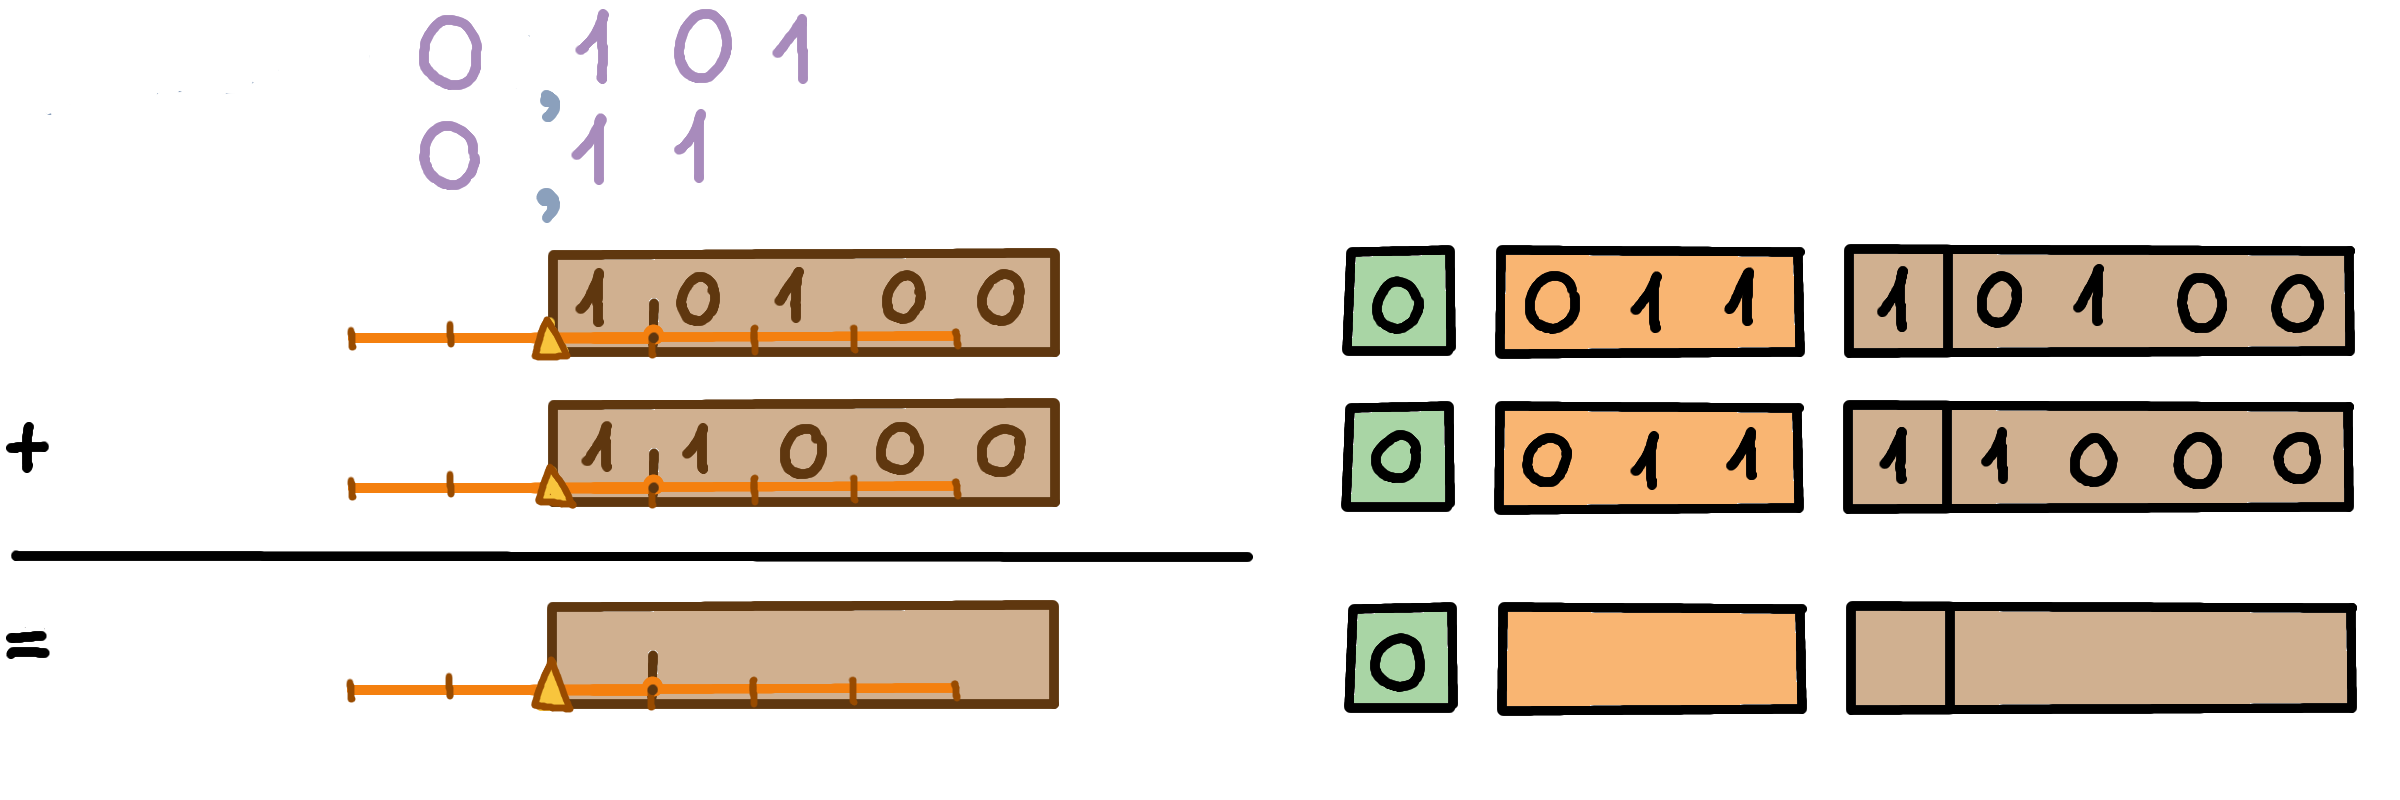
\includegraphics[width=\linewidth]{Pictures/Addition5-8and3-4_1.png}
\end{figure}
Da die zwei Kasten schon übereinander liegen, müssen wir sie nicht verschieben und können die Bits stellenweise zusammen addieren.
\begin{figure}[H]
\centering
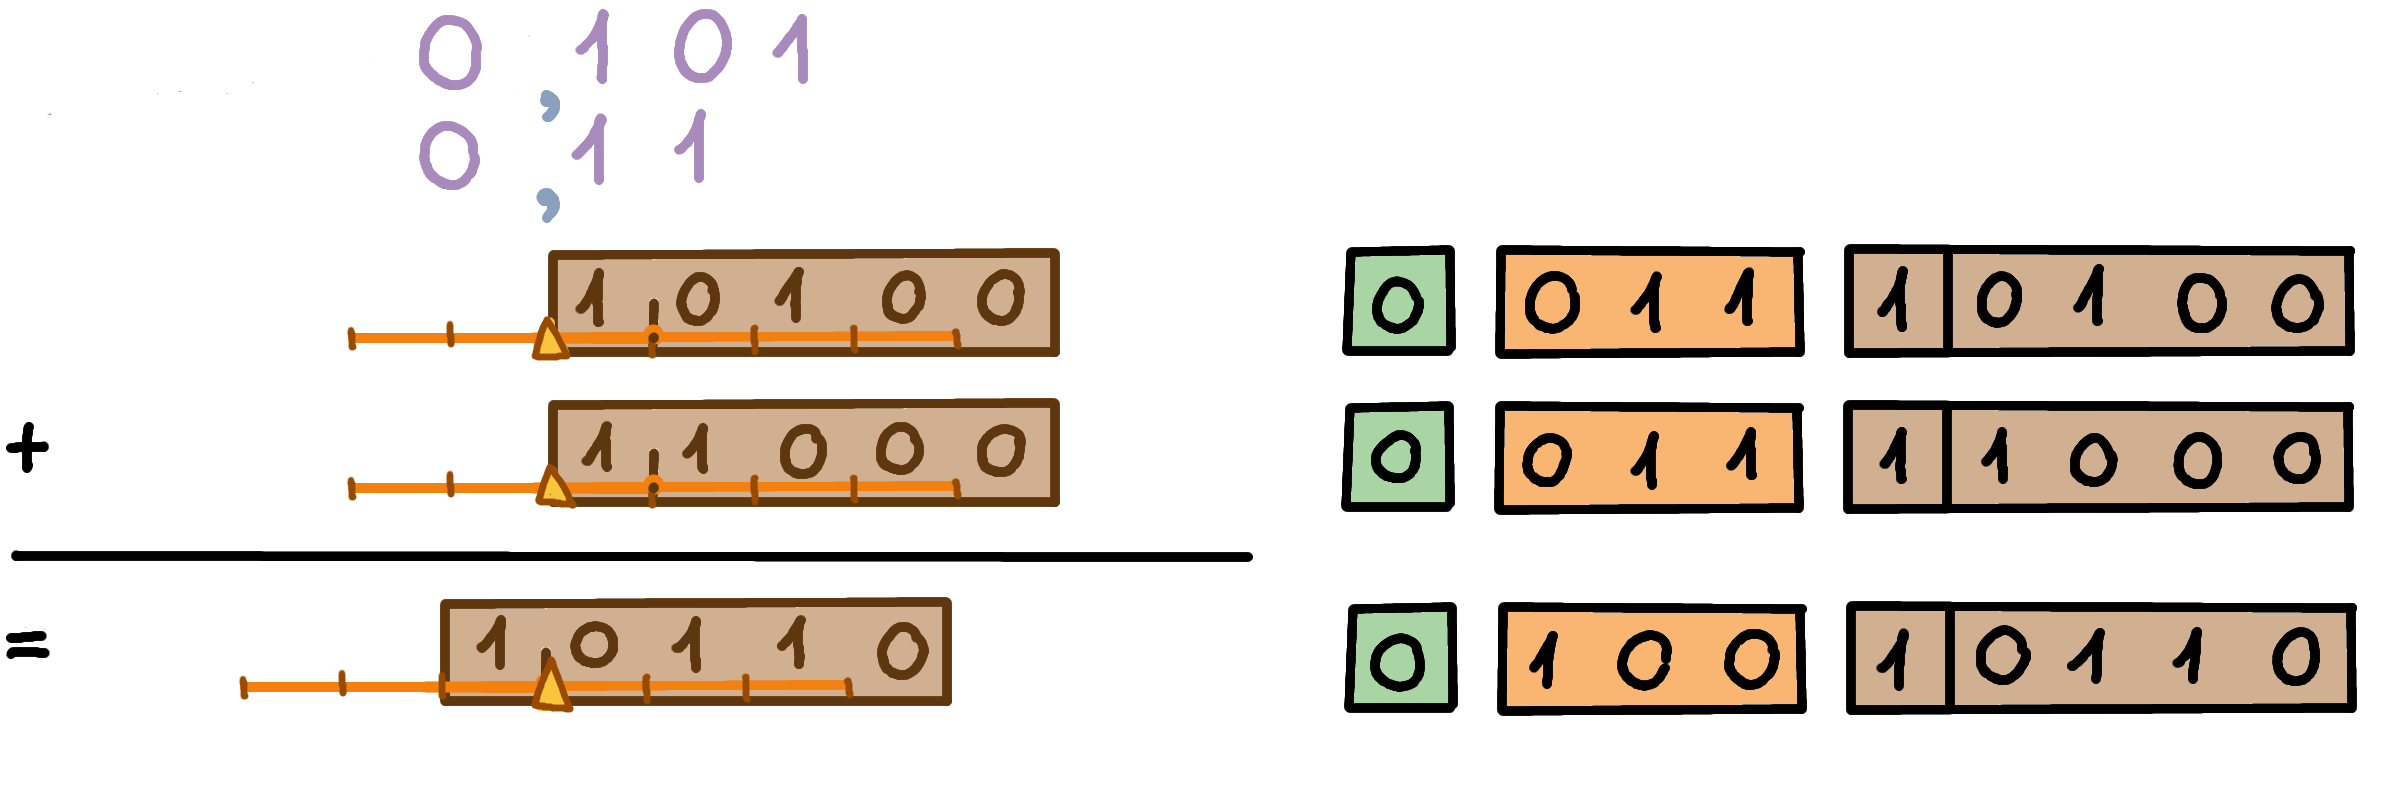
\includegraphics[width=\linewidth]{Pictures/Addition5-8and3-4_2.png}
\end{figure}
Der Kasten vom Ergebnis ist verschoben bezüglich den Kasten der Summanden.

\item \(10 + 2.25 = 12\), in der Exponentialschreibweise \(1.1000 \cdot 2^3\)

Im ersten Schritt schreiben wir die Zahlen auf.
\begin{figure}[H]
\centering
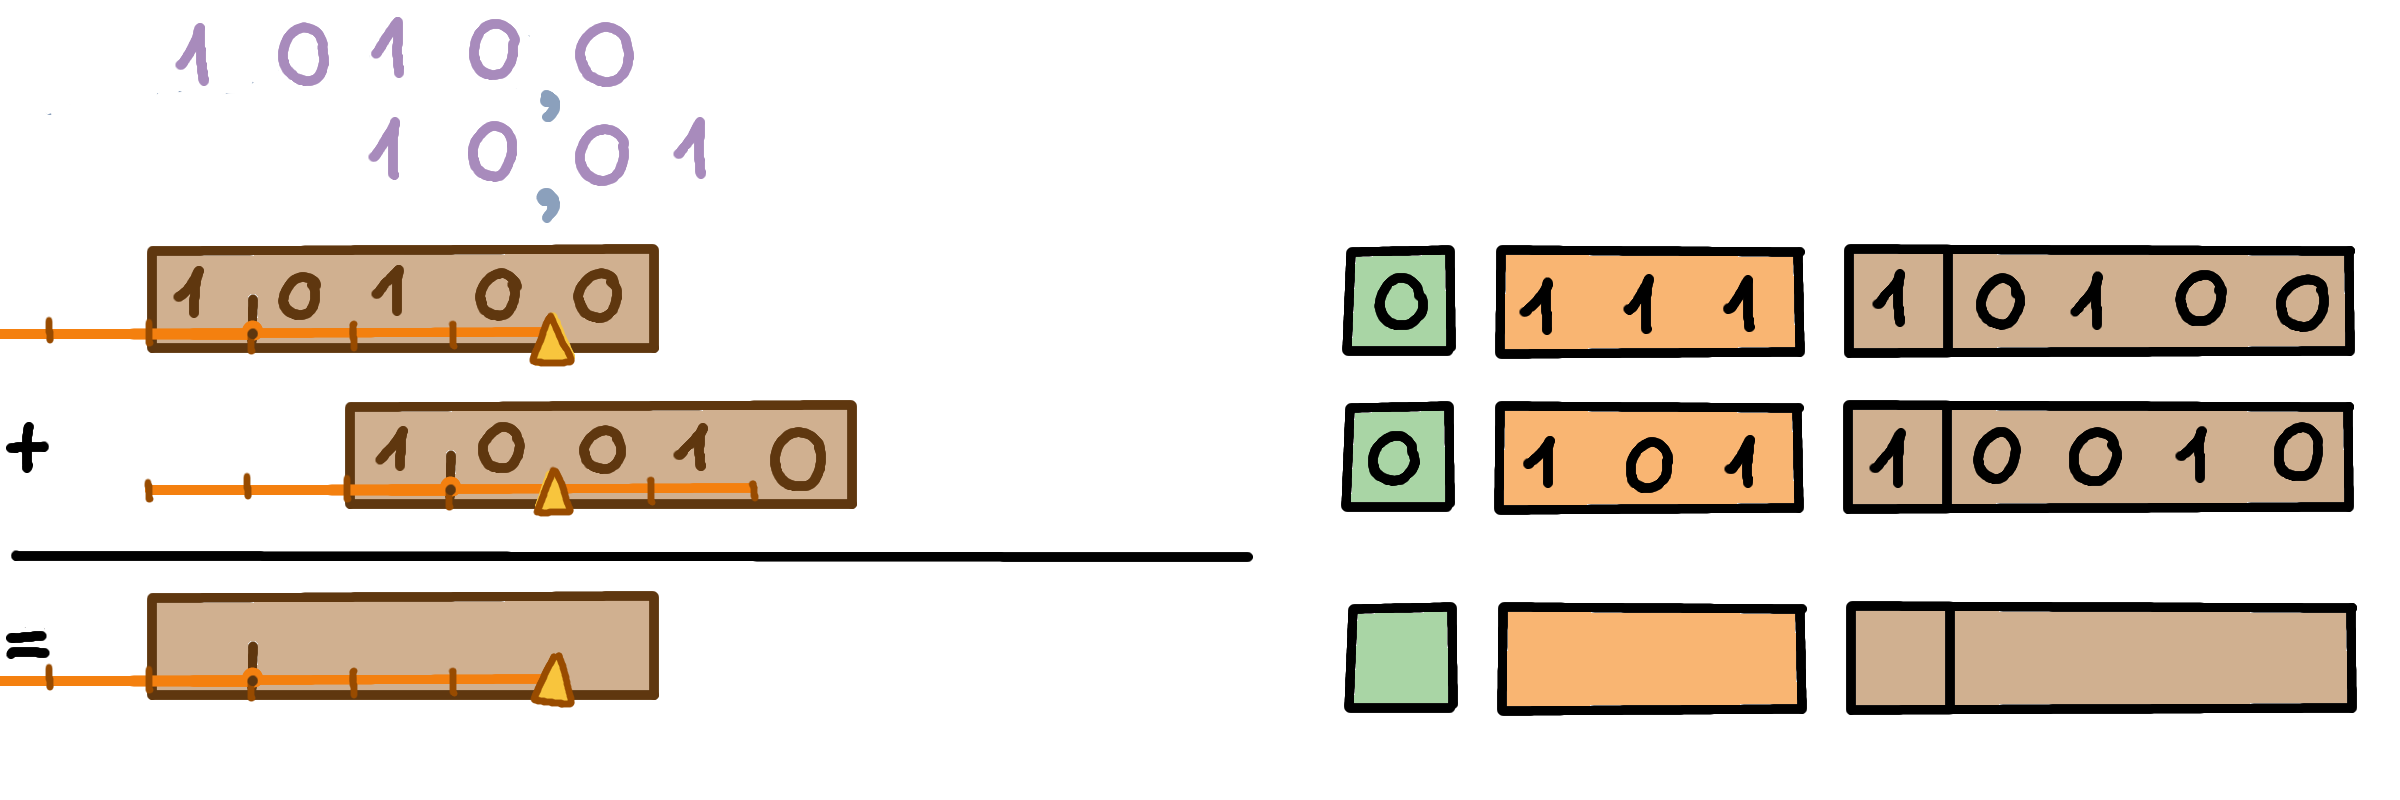
\includegraphics[width=\linewidth]{Pictures/Addition10and2-25_1.png}
\end{figure}

Im zweiten Schritt schiben wir den Kasten von der kleinsten Zahl unter den Kasten der grössten Zahl. Dabei gehen zwei Stellen verloren, eine davon ist eine Eins.
\begin{figure}[H]
\centering
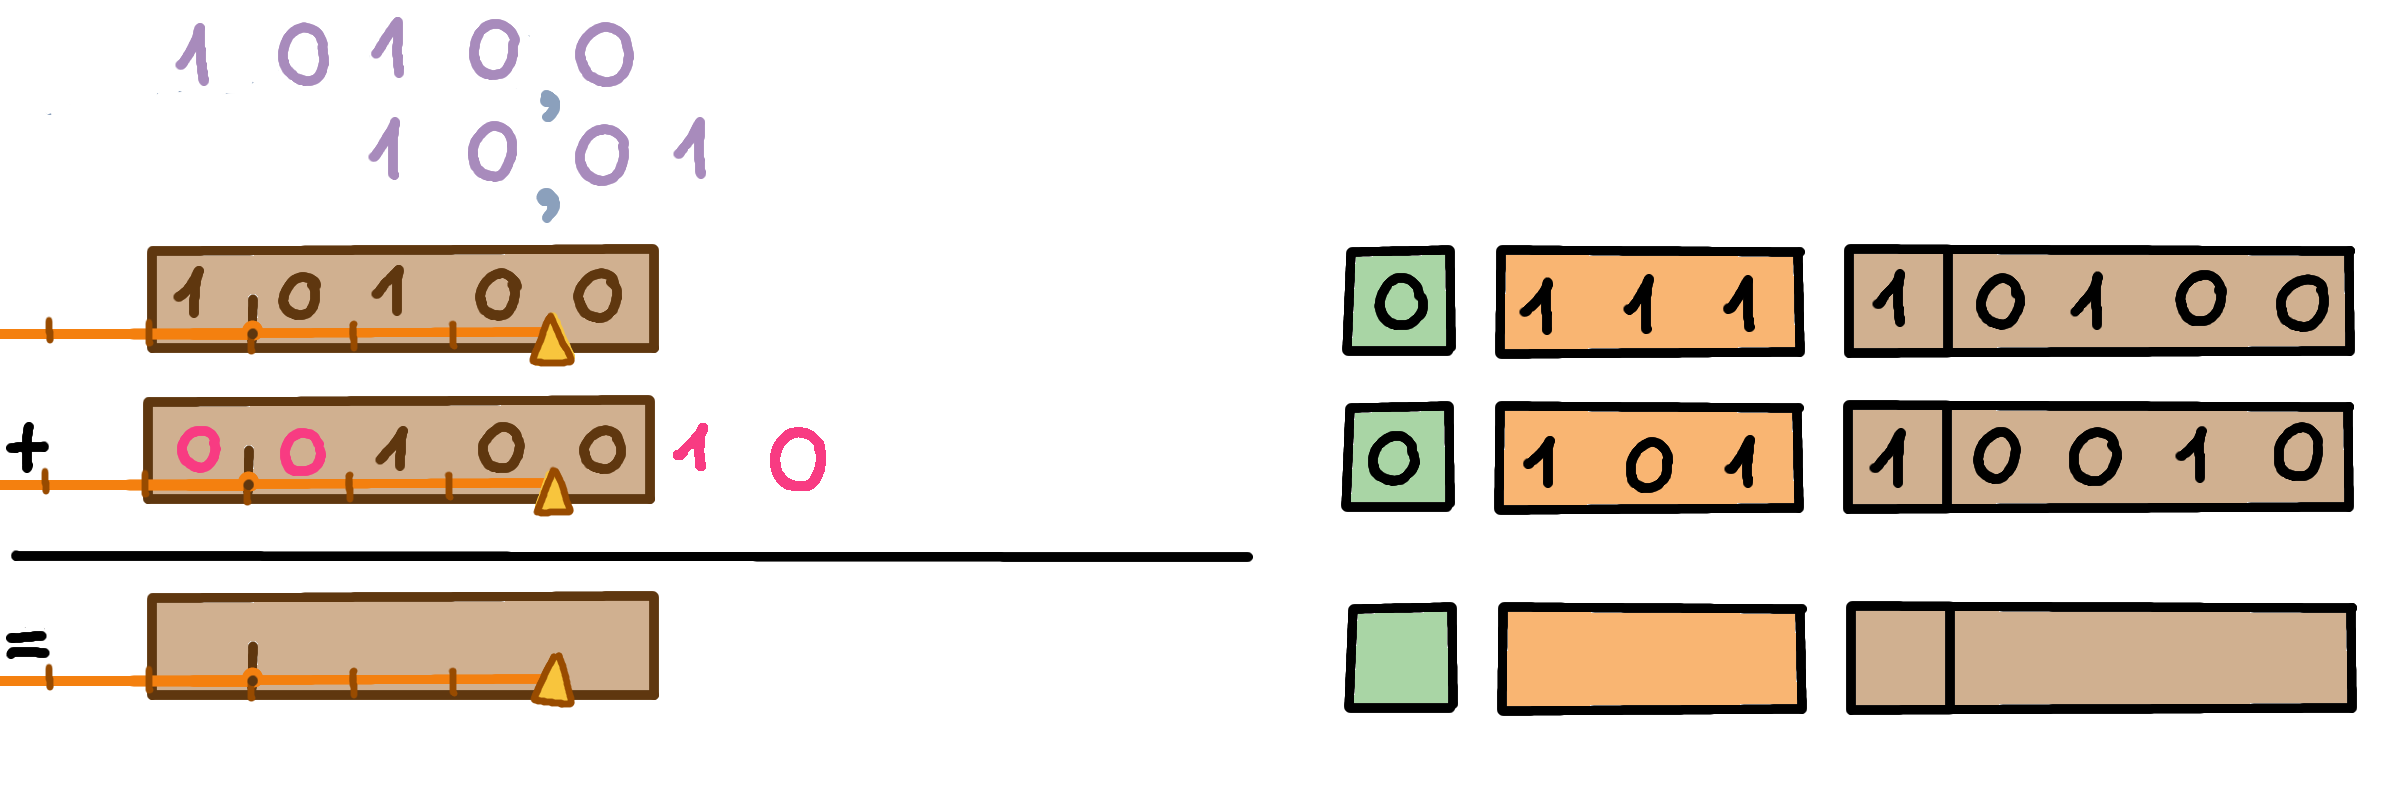
\includegraphics[width=\linewidth]{Pictures/Addition10and2-25_2.png}
\end{figure}

Nun können wir die Bits stellenweise zusammenrechnen.
\begin{figure}[H]
\centering
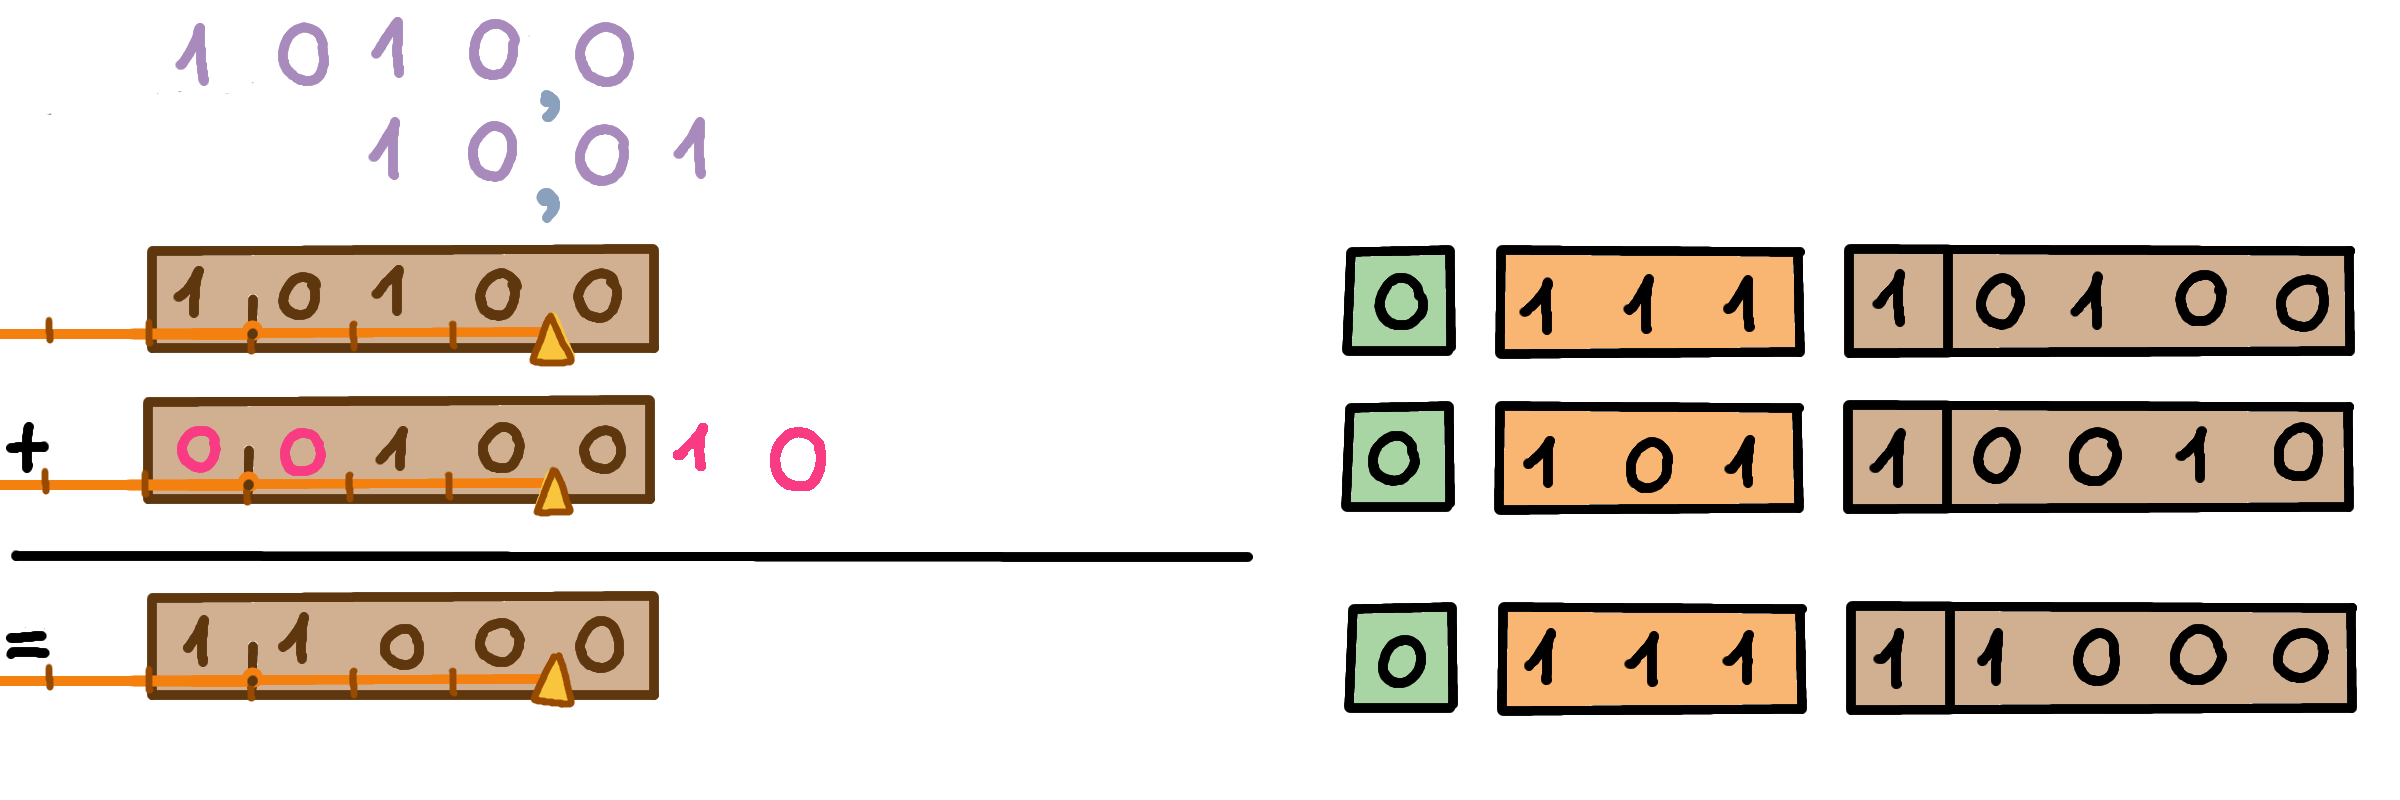
\includegraphics[width=\linewidth]{Pictures/Addition10and2-25_3.png}
\end{figure}

\item \(17/16 + 2 = 3\), in der Exponentialschreibweise \(1.1000 \cdot 2^1\).

Im ersten Schritt schreiben wir die Zahlen auf.
\begin{figure}[H]
\centering
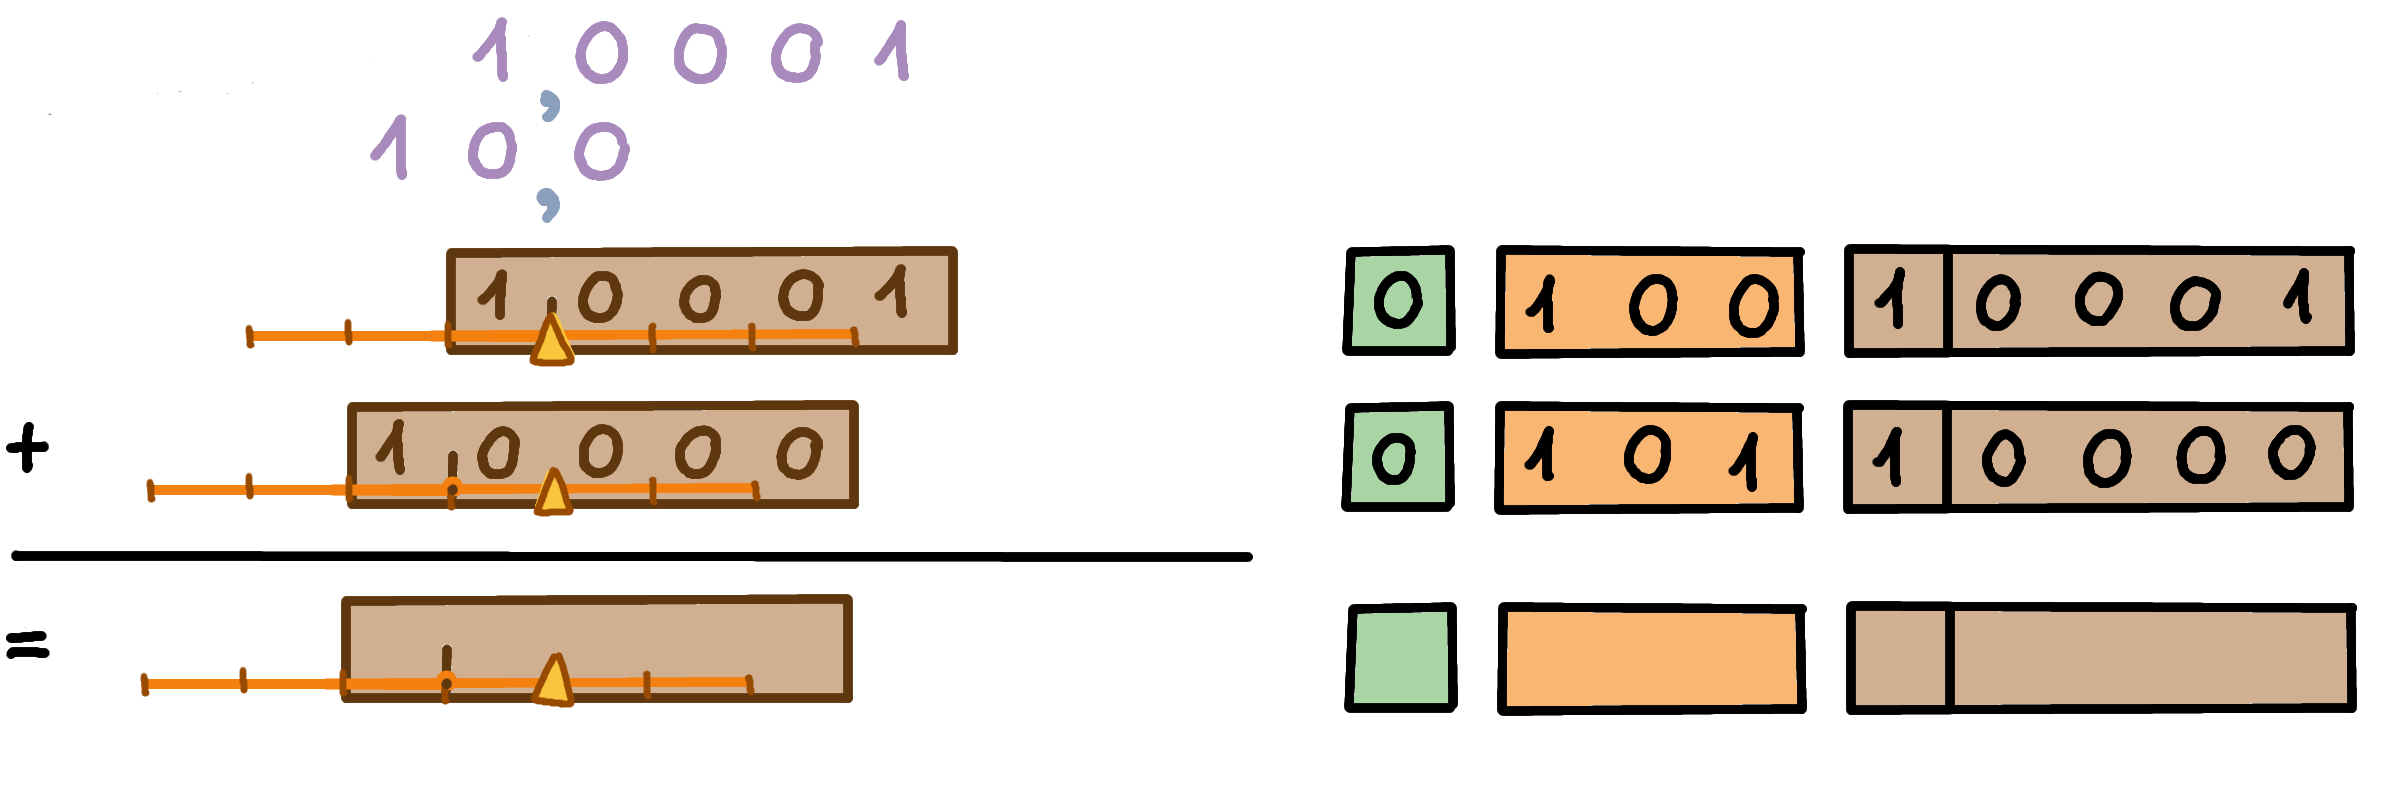
\includegraphics[width=\linewidth]{Pictures/Addition17-16and2_1.png}
\end{figure}

Im zweiten Schritt schiben wir den Kasten von der kleinsten Zahl unter den Kasten der grössten Zahl. Dabei geht eine Stelle verloren.
\begin{figure}[H]
\centering
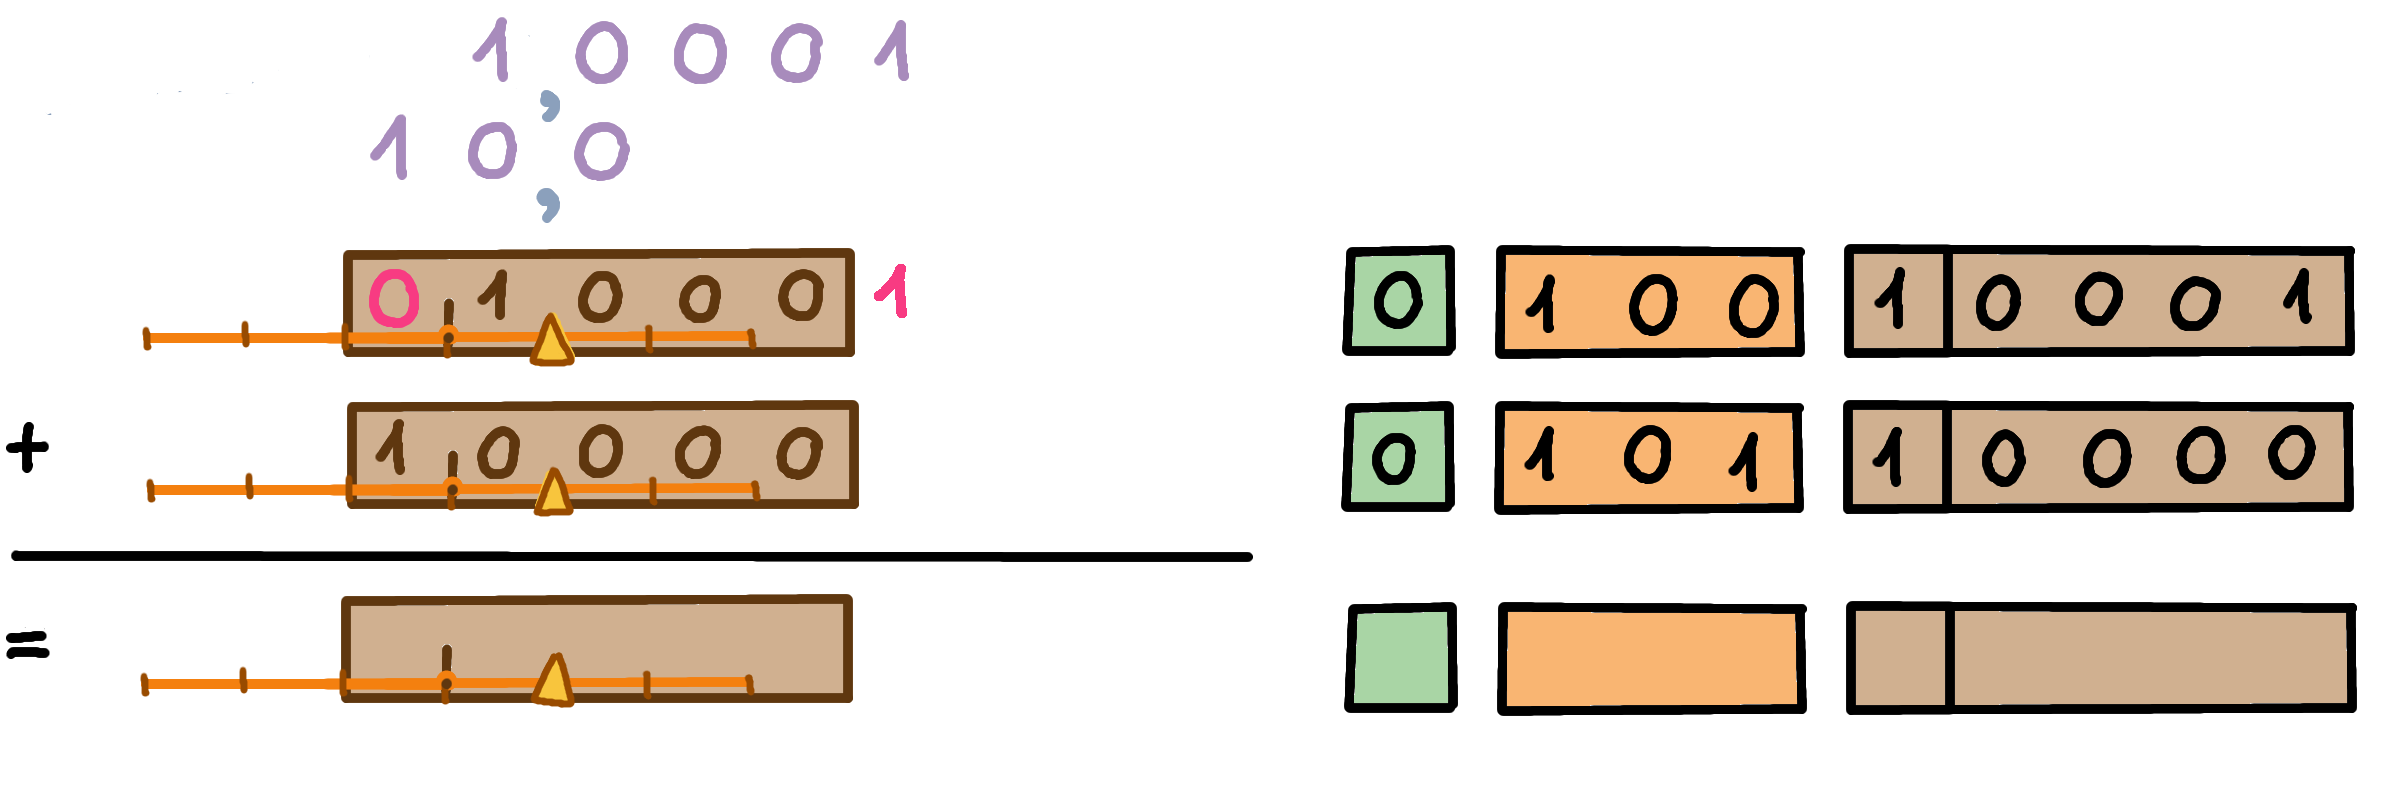
\includegraphics[width=\linewidth]{Pictures/Addition17-16and2_2.png}
\end{figure}

Nun können wir die Bits stellenweise zusammenrechnen.
\begin{figure}[H]
\centering
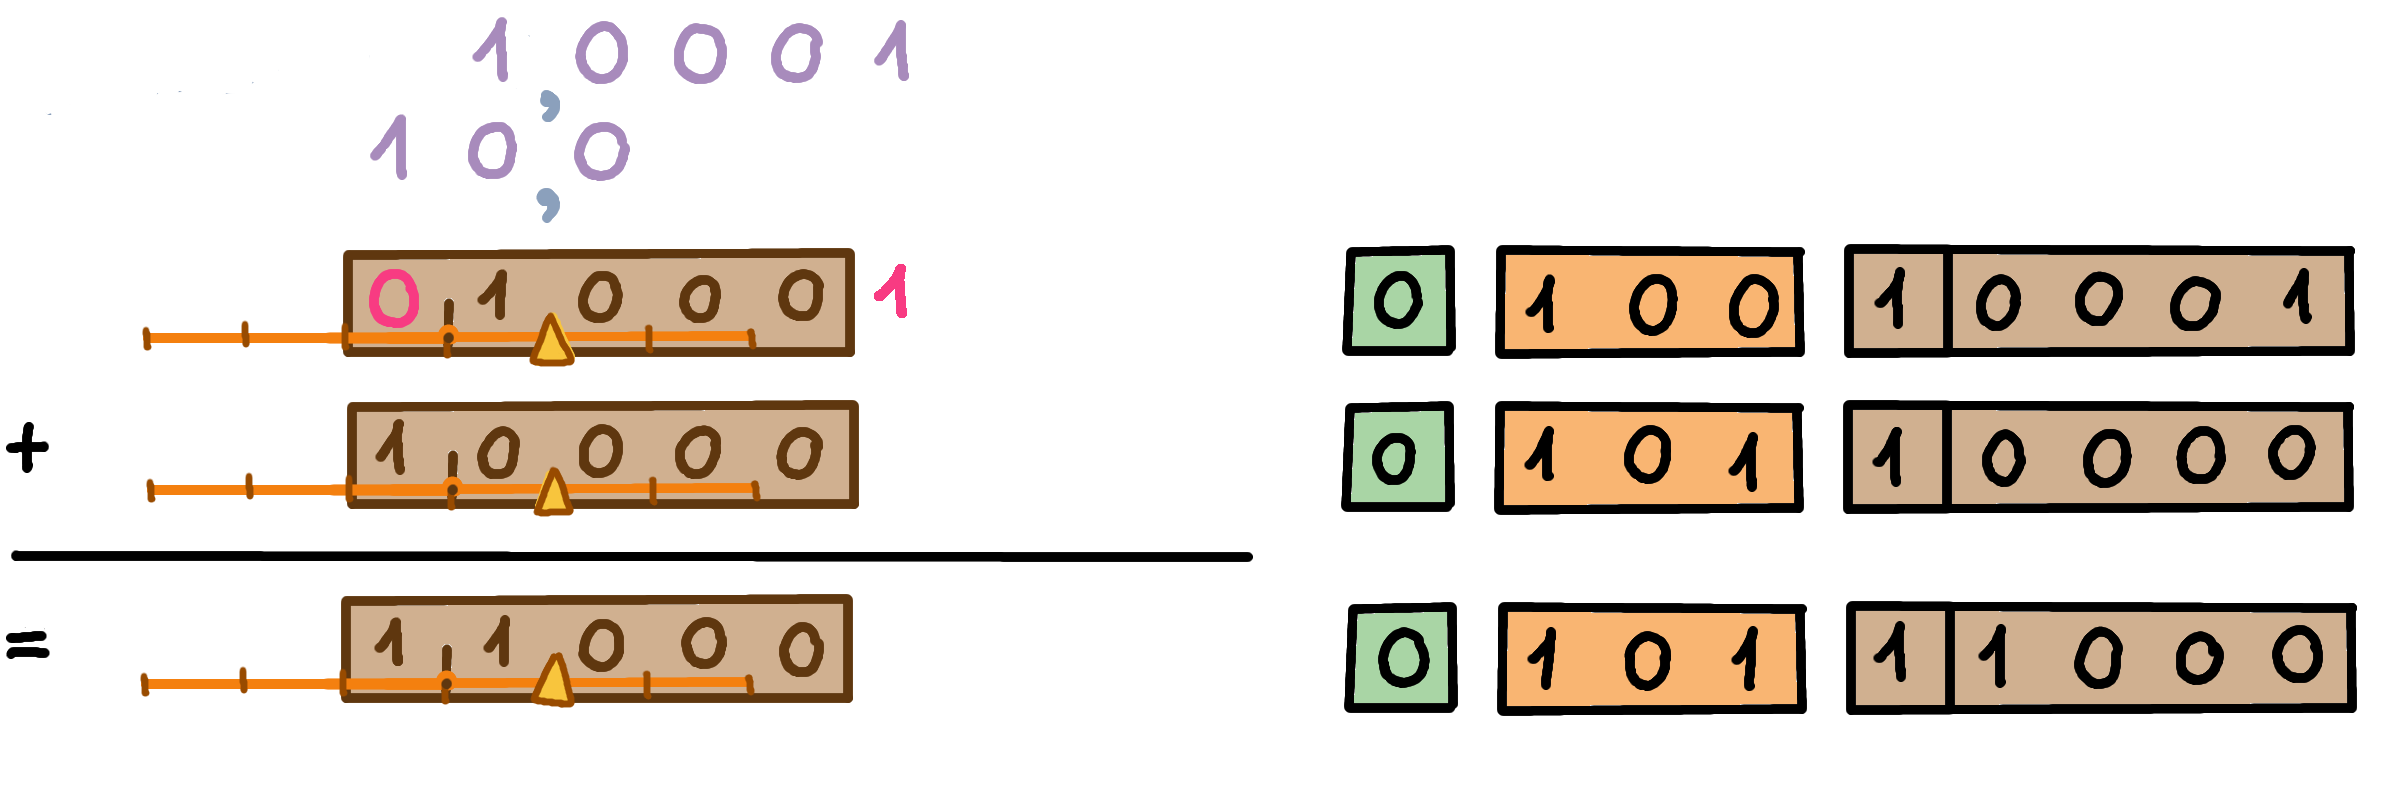
\includegraphics[width=\linewidth]{Pictures/Addition17-16and2_3.png}
\end{figure}

\end{enumerate}

%--------------------------------

\paragraph{Aufgabe \ref{ein_achtel}} Die maximale Zahl, die wir erreichen können, wenn wir \(1/8 + 1/8 + \dotsb + 1/8\) zusammen rechnen, ist \(4.0\).

Zum einen, wenn wir die \(4.0\) erreicht haben, kommen wir nicht mehr weiter.
Das sehen wir, wenn wir \(4.0 + 1/8\) ausrechnen. Wie gewöhnlich schreiben wir zuerst die Summanden untereinander.
\begin{figure}[H]
\centering
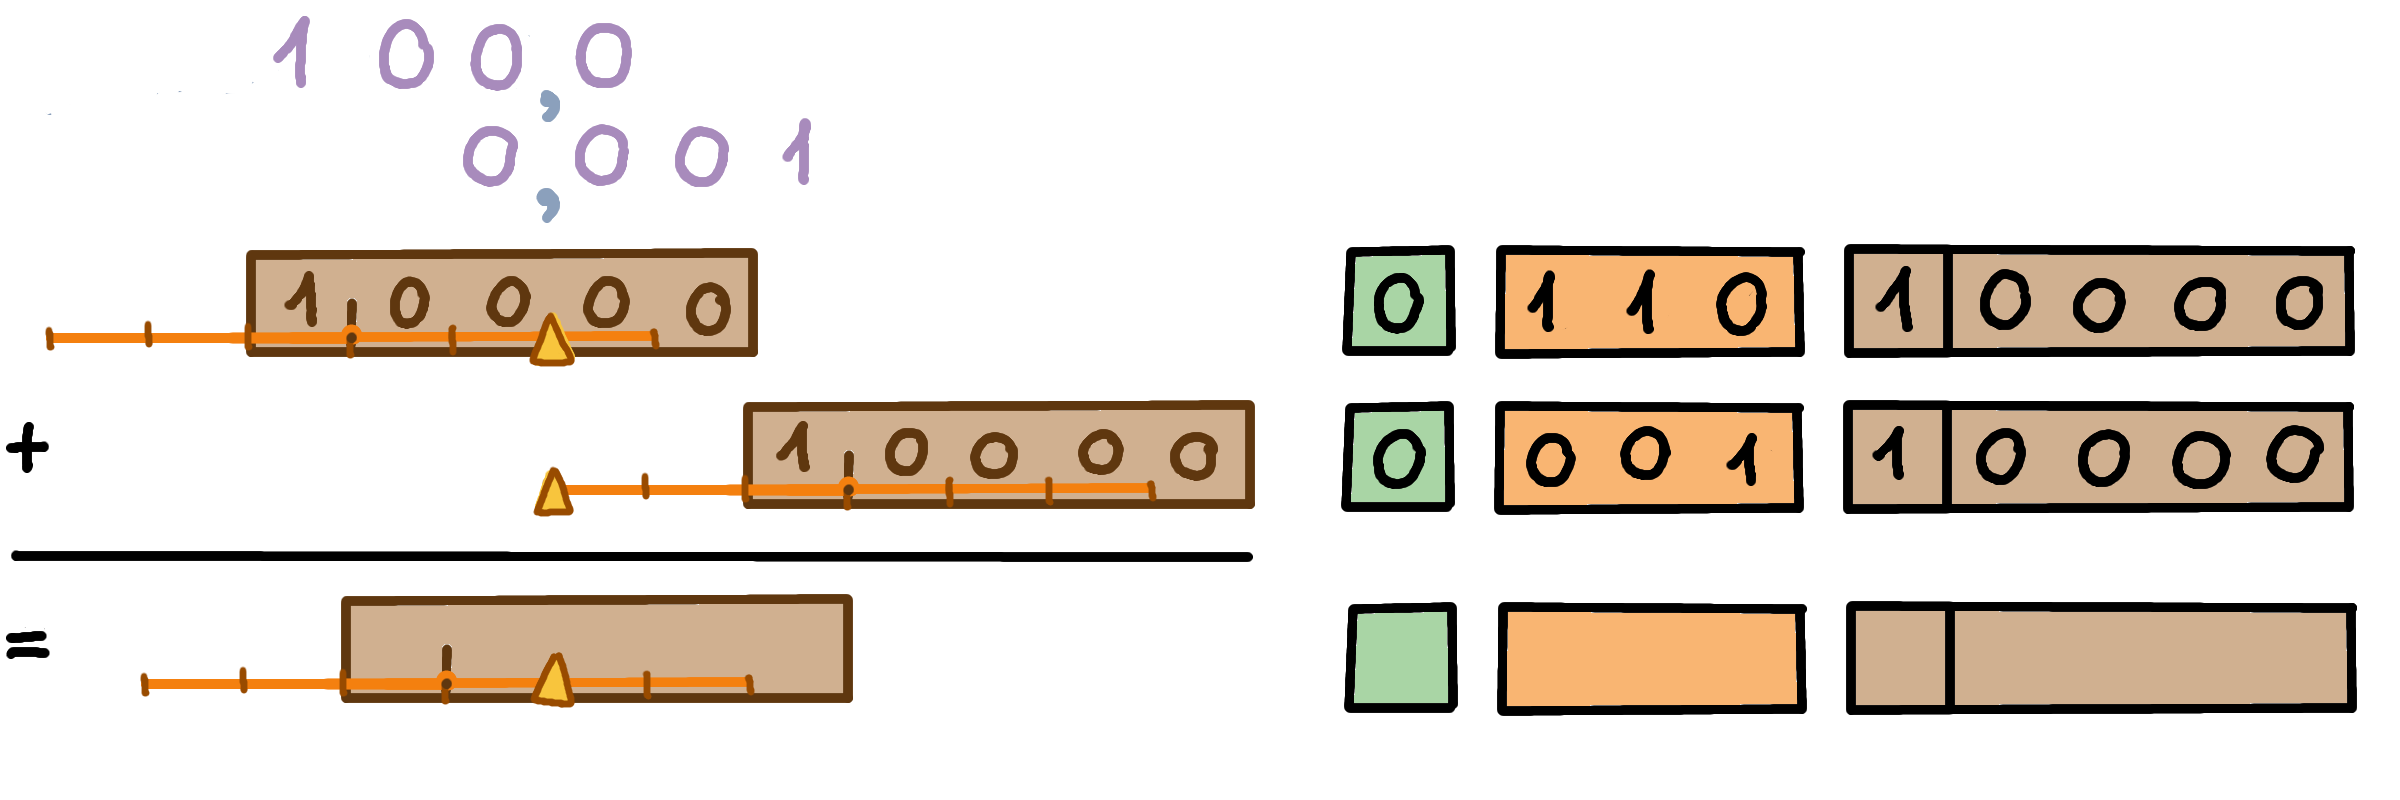
\includegraphics[width=\linewidth]{Pictures/Addition4and1-8_1.png}
\end{figure}
Wenn wir den Kasten von \(1/8\) unter den Kasten von \(4.0\) verschieben, sehen wir, dass alle signifikanten Stellen von \(1/8\) verloren gehen, auch die führende Eins.
\begin{figure}[H]
\centering
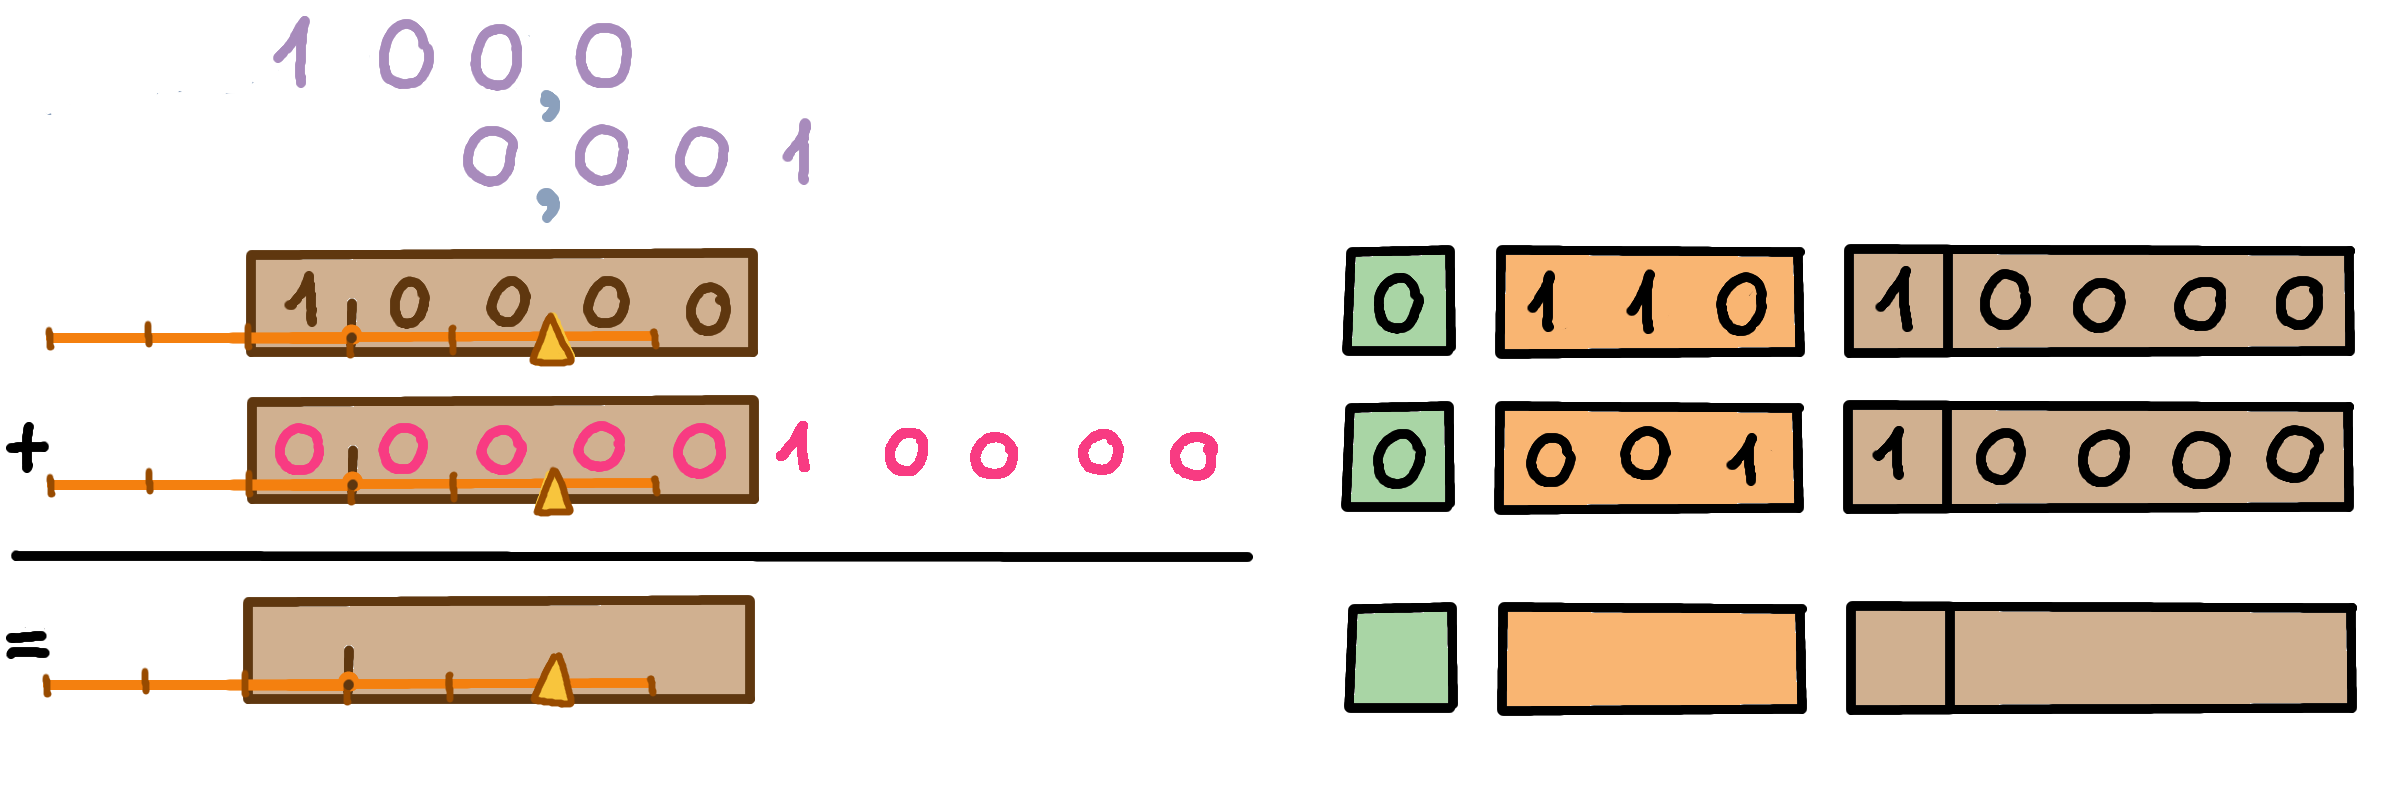
\includegraphics[width=\linewidth]{Pictures/Addition4and1-8_2.png}
\end{figure}
Deswegen, wenn wir \(4.0 + 1/8\) ausrechnen, kriegen wir \(4.0\).
\begin{figure}[H] 
\centering
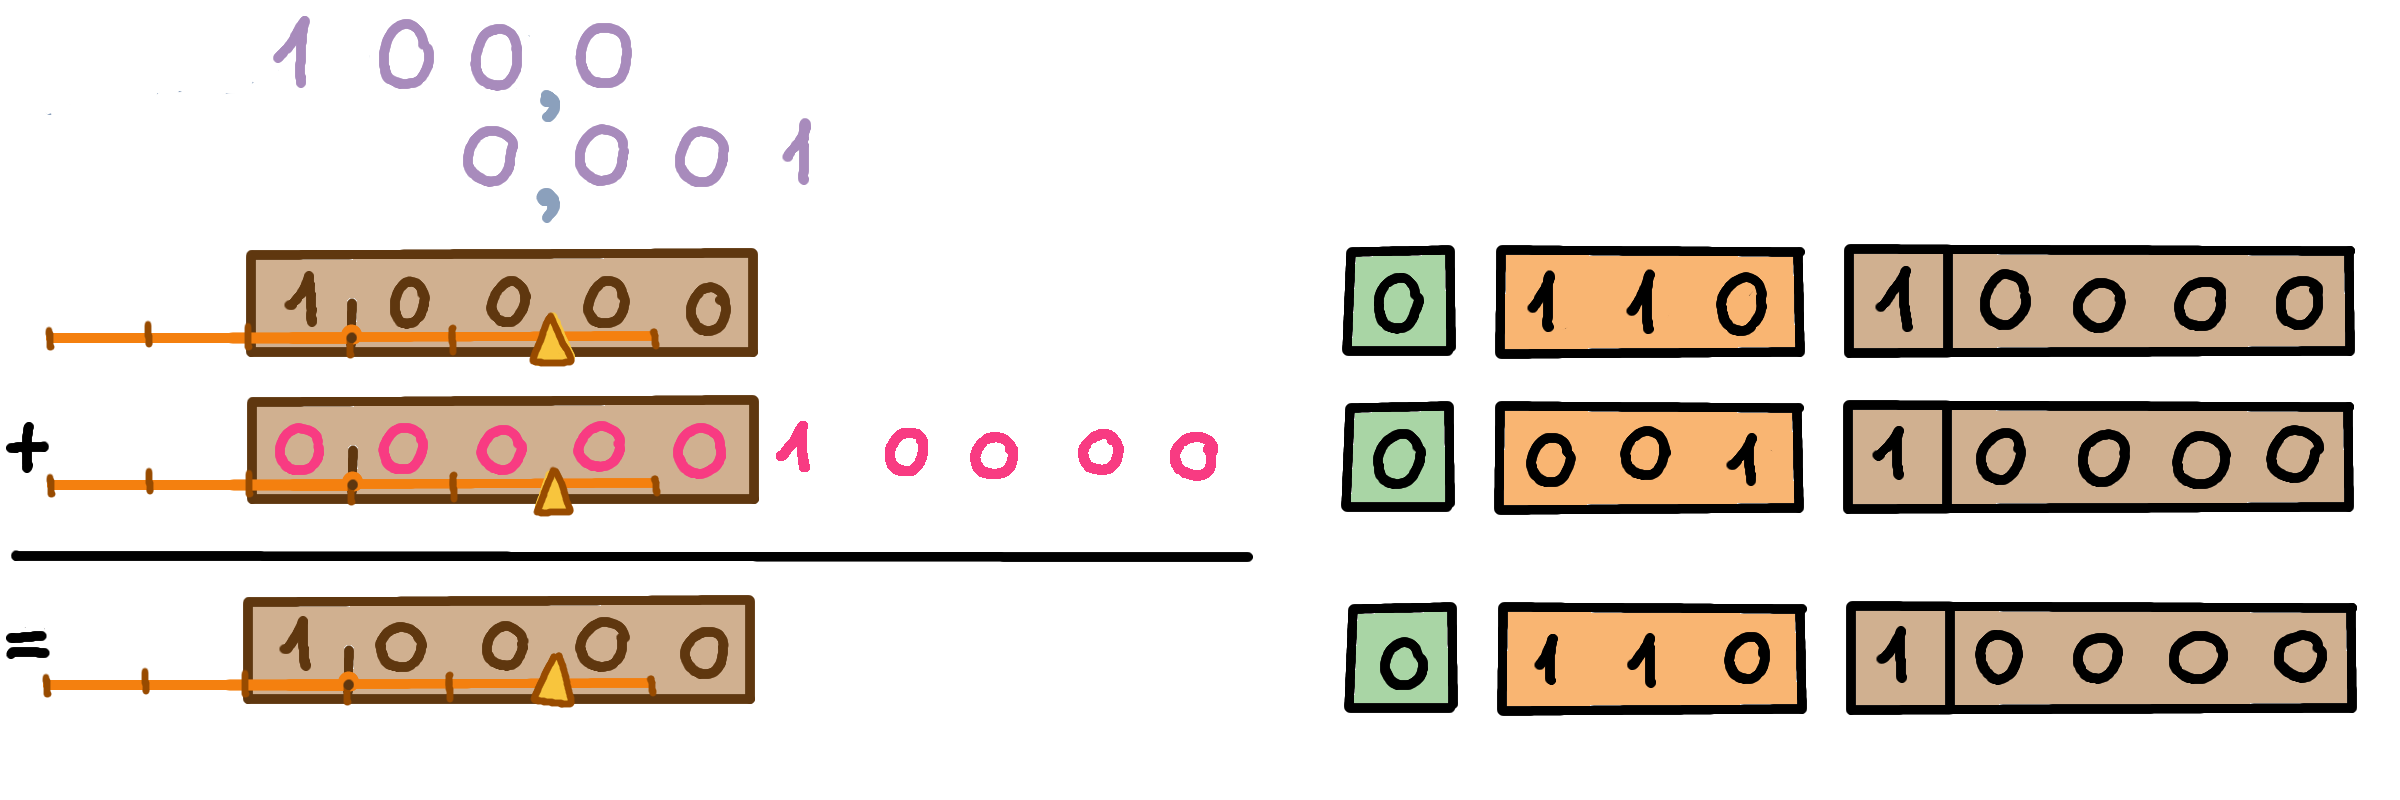
\includegraphics[width=\linewidth]{Pictures/Addition4and1-8_3.png} 
\end{figure}
Egal wie viele \(1/8\) rechnen wir zusammen, bleiben wir immer bei \(4.0\).

Jetzt bleibt uns zu zeigen, dass wir die \(4.0\) auch tatsächlich erreichen können. Das Problem bei der \(4.0\) ist, dass alle signifikanten Stellen von \(1/8\) verloren gehen. Das passiert, weil der Unterschied zwischen dem Exponenten von \(4.0\) und dem Exponenten von \(1/8\) die ganze Mantissenlänge beträgt. Das passiert bei einem kleineren Exponenten nicht. Zum Beispiel, wenn wir \(2.0 + 1/8\) ausrechnen, sehen wir, dass das Ergebnis wie erwartet \(17/8\) ist.

Um zu zeigen, dass das Problem erst bei \(4.0 + 1/8\) auftritt, rechnen wir \(2.0 + 1/8\). Das Ergebnis ist wie erwartet \(17/8\).
\begin{figure}[H]
\centering
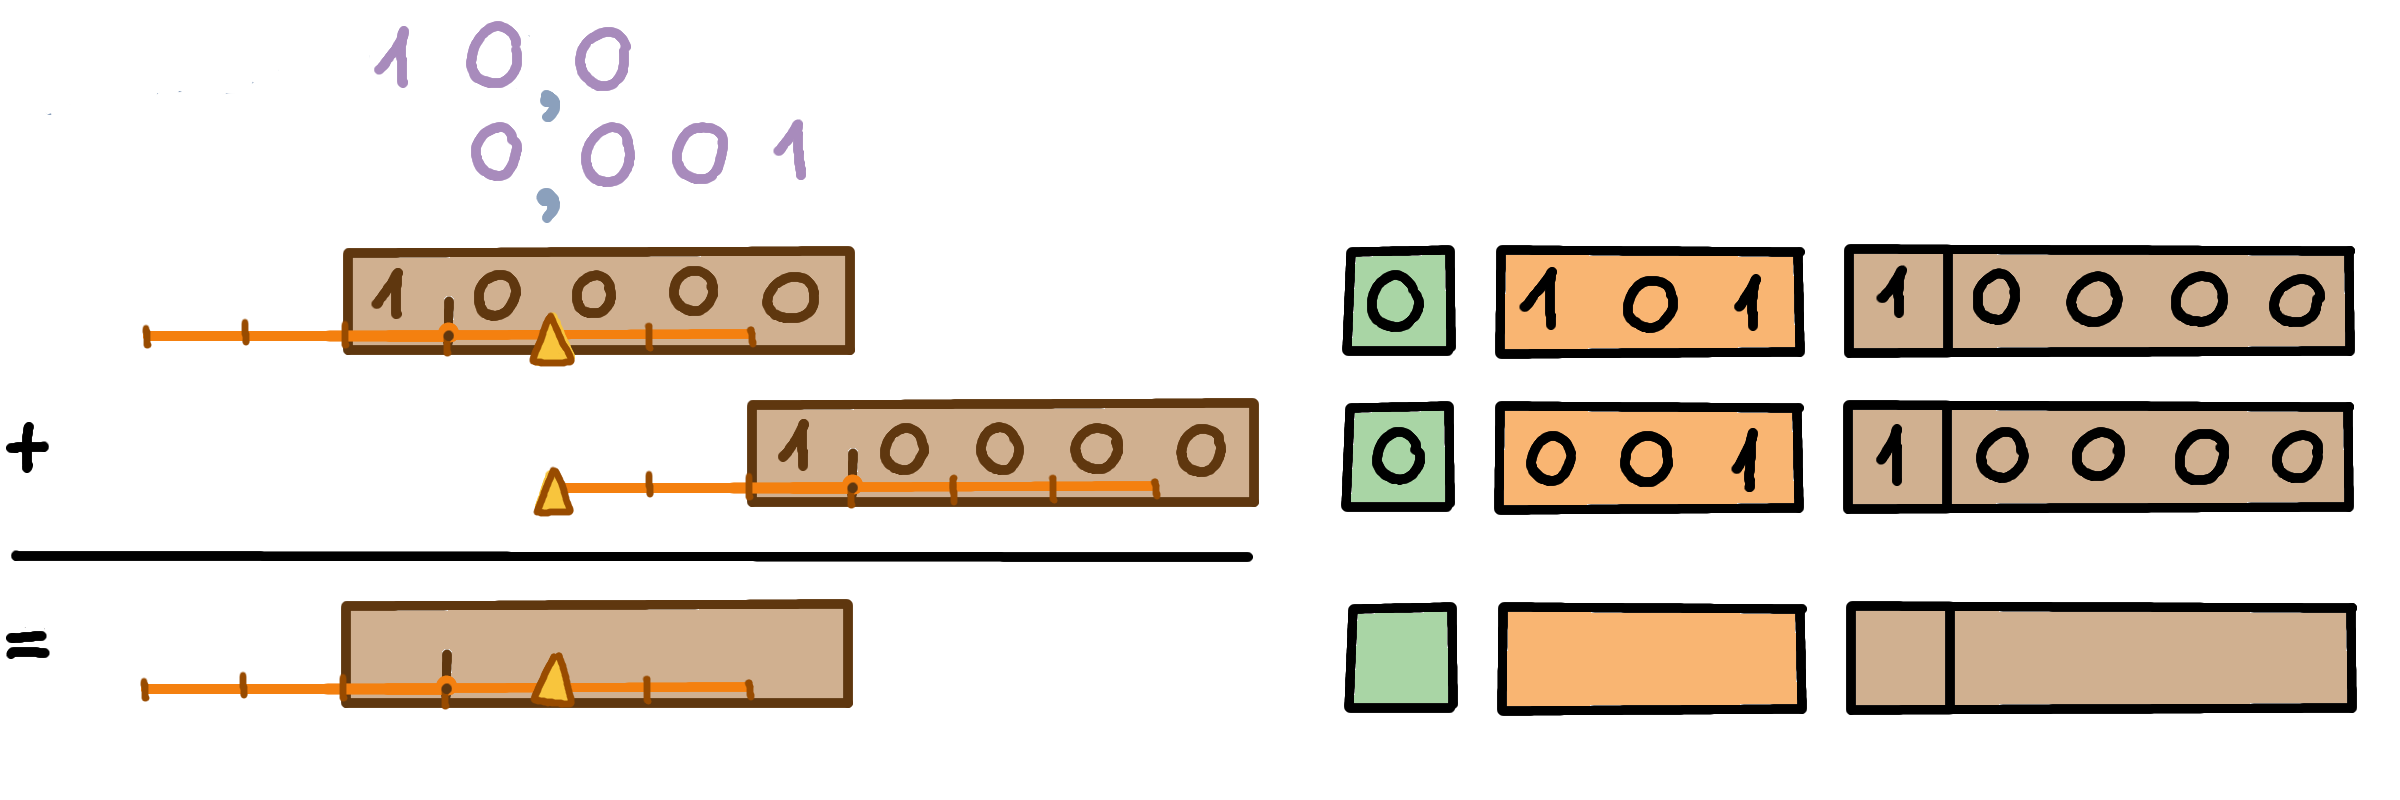
\includegraphics[width=\linewidth]{Pictures/Addition2and1-8_1.png} 
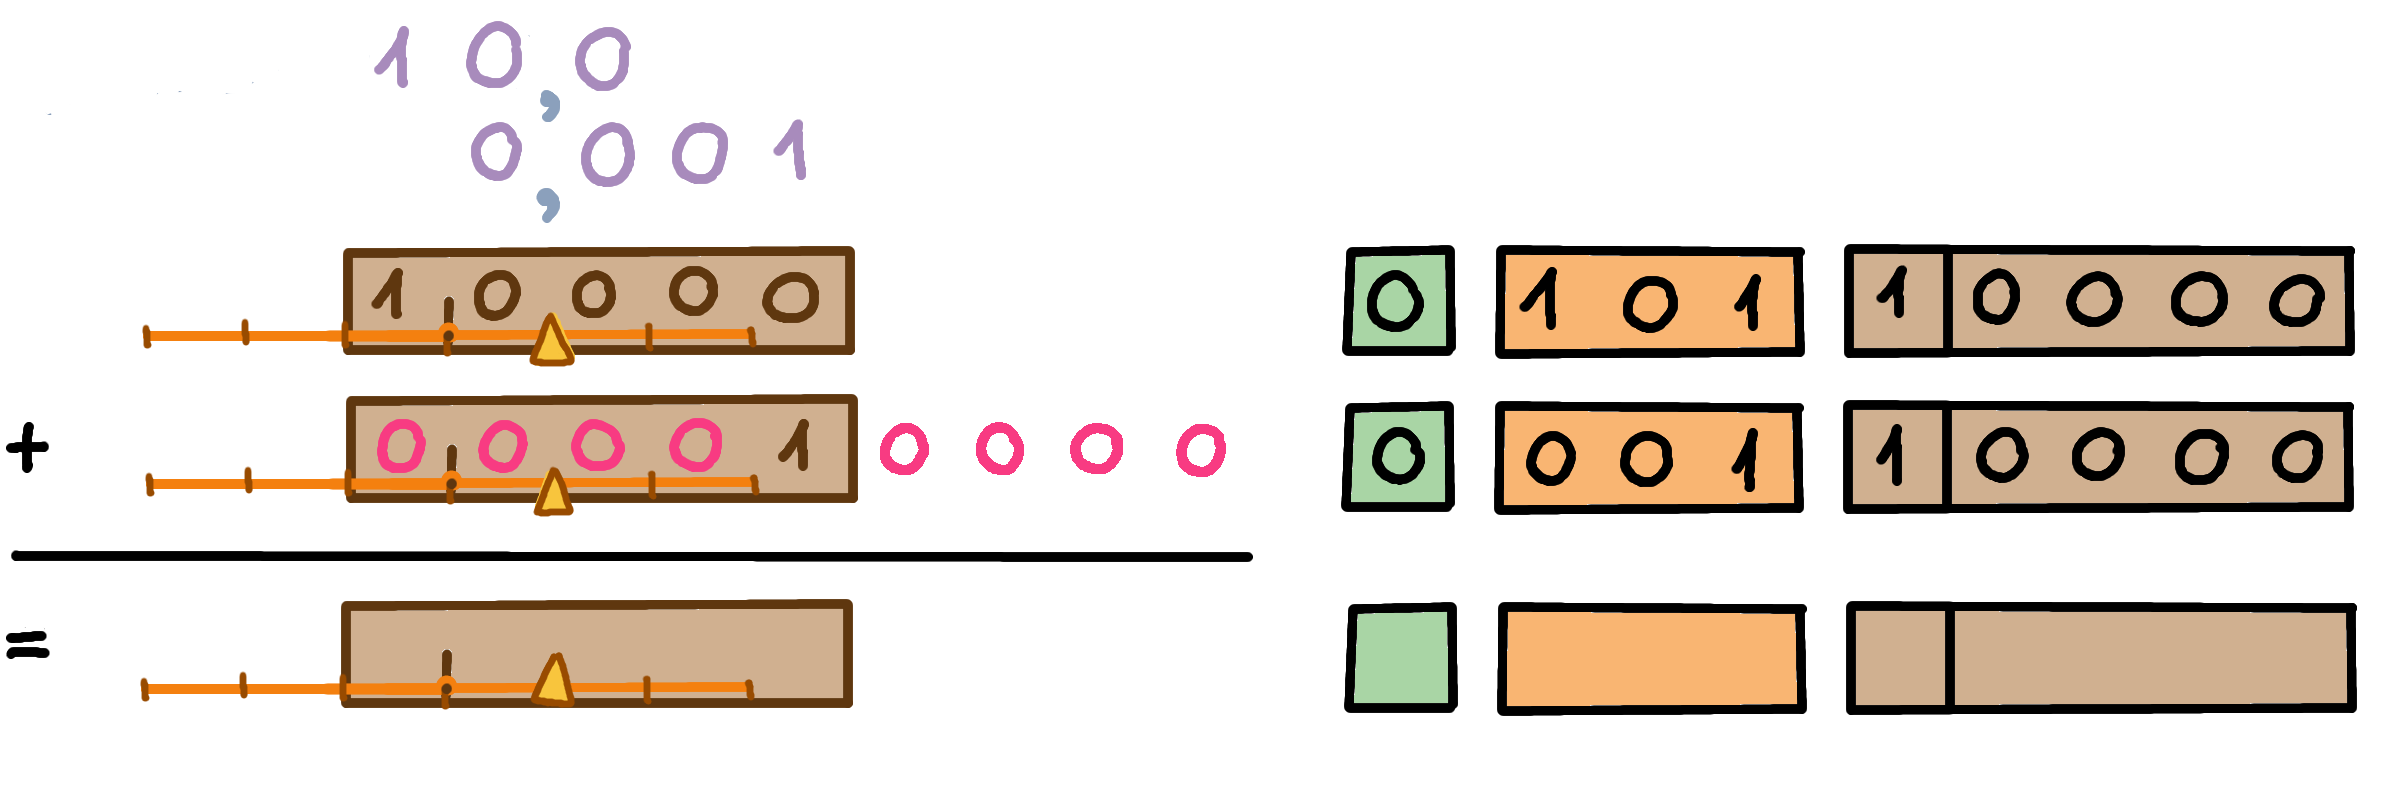
\includegraphics[width=\linewidth]{Pictures/Addition2and1-8_2.png} 
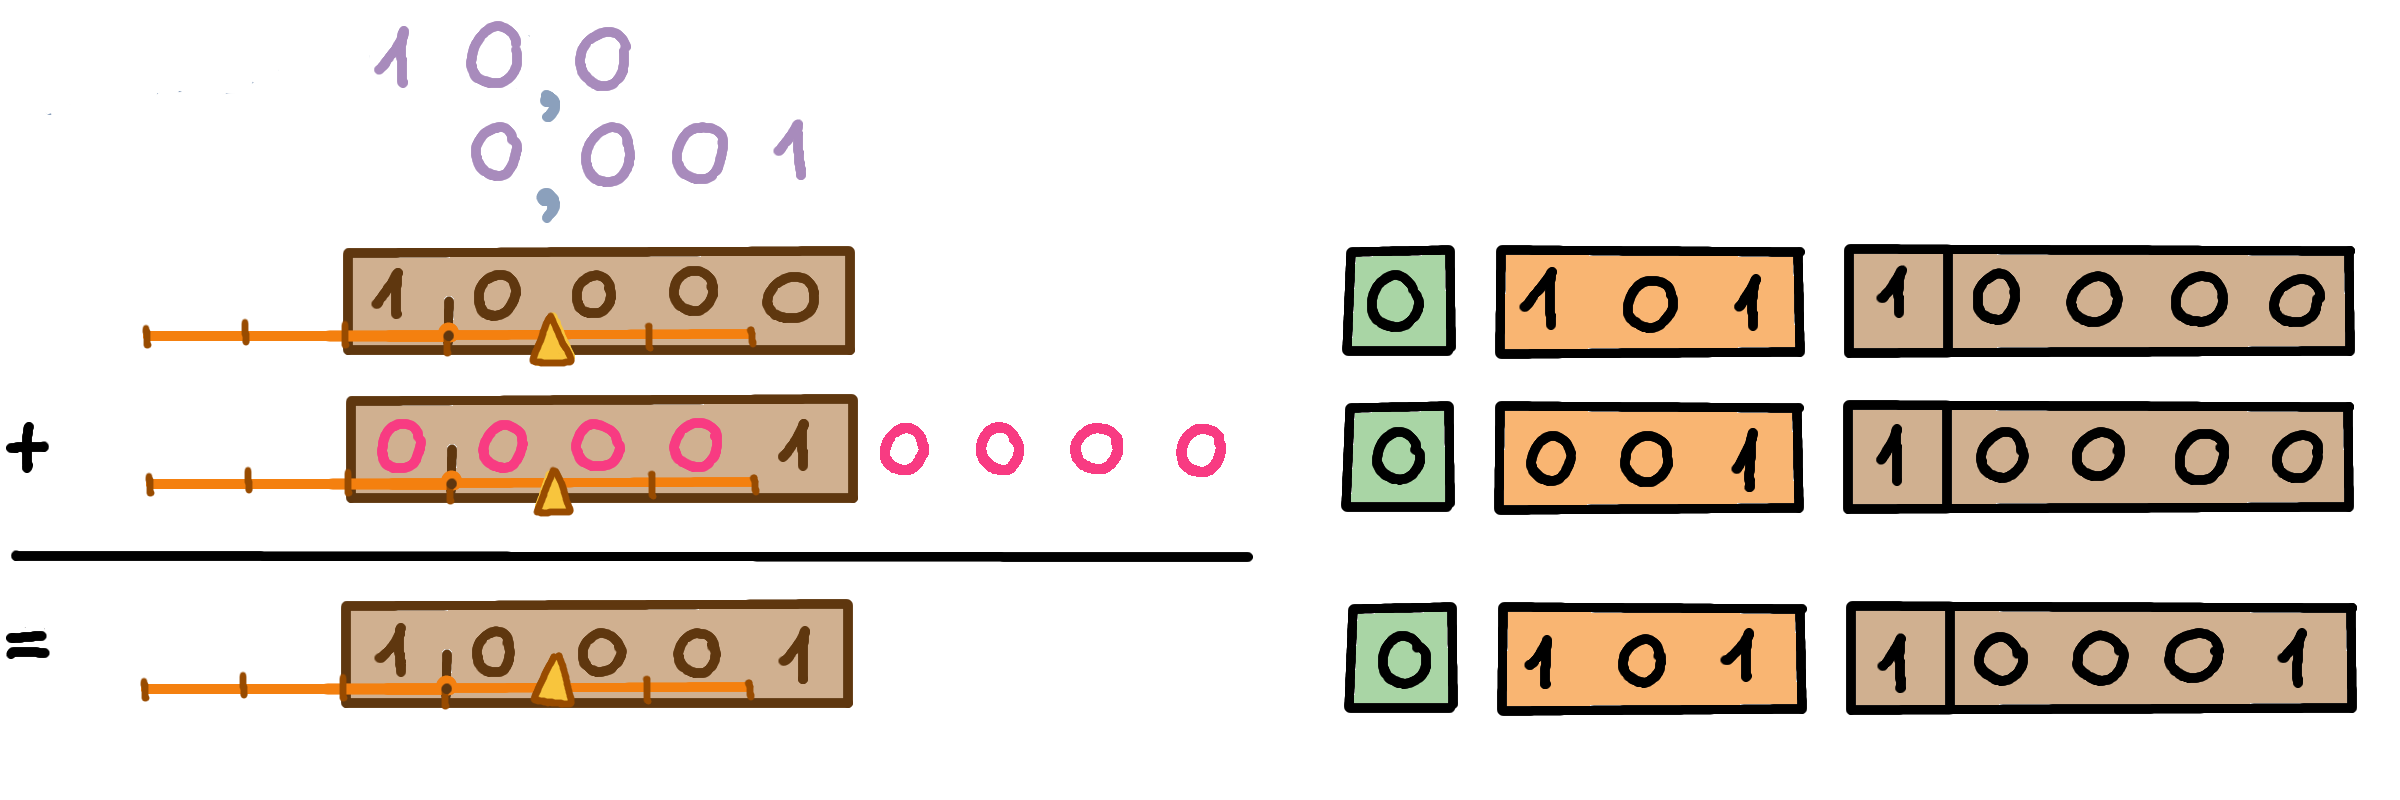
\includegraphics[width=\linewidth]{Pictures/Addition2and1-8_3.png} 
\end{figure}
Wir erreichen also die \(4.0\) nach 32 Summanden und kommen dann nicht mehr weiter.

%--------------------------------

\paragraph{Aufgabe \ref{addition_kontrollfragen}}
\begin{enumerate}[(a)]
\item Der Wert der Bits in der Mantisse hängt vom Exponenten ab. Zum Beispiel, dieselbe Mantisse \(1.0000\) mit unterschiedlichen Exponenten kann \(4\), \(2\), \(1\), \(1/2\), \(1/4\) und \(1/8\) darstellen. Wir wollen nicht, dass \(1+2\) das gleiche Ergebnis liefert die \(1 + 1/4\). Wir wollen nur Bits mit dem gleichen Wert zusammen addieren. Deswegen müssen wir vor der Addition sicherstellen, dass die Kasten der beiden Summanden exakt untereinander stehen.

\item Die Aussage von Gregory ist falsch. Der Kasten vom Ergebnis kann sich bewegen bezüglich des Kastens vom grössten Summanden. Dies passiert, zum Beispiel, wenn man \(2.5 + 1.75\) ausrechnet.

\item Hannah hat teilweise recht. Die Addition bei den Fliesskommazahlen ist kommutativ aber nicht assoziativ.

Wenn wir zwei Zahlen zusammen addieren und diese zwei Zahlen vertauschen, kriegen wir das gleiche Ergebnis auch bei Fliesskommazahlen.

Wenn wir aber die Reihenfolge verändern, in welcher die Zahlen zusammengerechnet werden, können wir unterschiedlich Ergebnisse bekommen. Das passiert, weil wir nur dann den exakten Wert ausrechnen können, wenn die Grössenordnung der Teilsummanden ähnlich ist.
\end{enumerate}

%--------------------------------

\paragraph{Aufgabe \ref{ameisenkönigin}}

Nein, das Programm der Ameisenkönigin wird unendlich lange laufen und die Anzahl Ameisen, die es braucht, um 10 Reiskörnchen zu transportieren, nie ausgeben. Das Problem ist analog zu dem, was wir in Aufgabe \ref{ein_achtel} gesehen haben. Das Programm läuft wie erwartet bis wir die \(8.0\) erreichen. Wenn wir aber \(1/4\) dazu rechnen, dann verlieren wir alle signifikanten Stellen von \(1/4\) und die \(8.0\) bleibt unverändert.
\begin{figure}[H]
\centering
\includegraphics[width=\linewidth]{Pictures/Addition8and1-4_1.png} 
\includegraphics[width=\linewidth]{Pictures/Addition8and1-4_2.png} 
\includegraphics[width=\linewidth]{Pictures/Addition8and1-4_3.png} 
\end{figure}

\end{document}
